\documentclass[../../main.tex]{subfiles}

\setcounter{footnote}{0} 

\newcommand{\taua}{$\tau_\text{acc}$ }
\newcommand{\tauns}{$\tau_\text{acc}$}

\NewDocumentCommand{\class}{v}{%
	\texttt{\textcolor{black}{#1}}%
}



\begin{document}
\vspace{-0.2cm}
\section{Manuscript IV}
{{\emph{A transferable active-learning strategy for reactive molecular force fields}}}

\subsection{Abstract}

Predictive molecular simulations require fast, accurate and reactive interatomic potentials. Machine learning offers a promising approach to construct such potentials by fitting energies and forces to high-level quantum-mechanical data, but doing so typically requires considerable human intervention and data volume. Here we show that, by leveraging hierarchical and active learning, accurate Gaussian Approximation Potential (GAP) models can be developed for diverse chemical systems in an autonomous manner, requiring only hundreds to a few thousand energy and gradient evaluations on a reference potential-energy surface. The approach uses separate intra- and inter-molecular fits and active learning to maximise a prospective error metric used to quantify accuracy. We demonstrate applications to a range of molecular systems: from bulk solvents, a solvated metal ion and a metallocage onwards to chemical reactivity, including a bifurcating Diels–Alder reaction in the gas phase and non-equilibrium dynamics (S${}_\text{N}$2 reaction) in explicit solvent. The method provides a route to routinely generating machine-learned force fields for reactive molecular systems. 


\subsection{Introduction}

Molecular simulations are a cornerstone in computational chemistry, providing dynamical insights beyond experimental resolution.\cite{Frenkel2002} Realistic simulations of (bio)chemical reactions require the inclusion of the chemical environment where they occur (e.g. solvent and/or enzyme) and often extended timescales. Therefore, the generation of accurate and efficient approaches has been central to the development of this field.

Empirical interatomic potentials (force fields), in combination with molecular dynamics (MD) or Monte Carlo (MC) simulations, have been widely used to sample the potential-energy surface (PES). However, they are limited in accuracy and transferability.\cite{Lindorff-Larsen2012} Moreover, most of these potentials are parameterised for isolated entities with fixed connectivity and thus unable to describe bond breaking/forming processes. In contrast, ab initio methods provide an accurate description of the PES, which is particularly critical for reactions in solution. However, because of their high computational cost and unfavourable scaling behaviour, they are limited to a few hundred atoms and simulation times of picoseconds in ab initio molecular dynamics (AIMD) at the DFT level, and practically impossible at the computational ‘gold-standard’ [CCSD(T)].\cite{Iftimie2005} 

Machine learning (ML) approaches have the potential to revolutionise force-field based simulations, aiming to provide the best of both worlds,\cite{Noe2020, Mueller2020, Unke2020} and have indeed begun to provide new insights into a range of challenging research problems.\cite{Khaliullin2011, Sosso2013, Niu2020, Cheng2020nature, Deringer2021, Ang2021, Cole2020, Rufa2020, Gastegger2017, Li2021} The development of an ML potential applicable to the whole periodic table mapping nuclear coordinates to total energies and forces is, however, precluded by the curse of dimensionality. Within small chemical subspaces, models can be achieved using neural networks (NNs),\cite{Unke2020, Behler2007, Behler2017, Smith2017, Schutt2017, Unke2019} kernel-based methods such as the Gaussian Approximation Potential (GAP) framework\cite{Bartok2010, Bartok2015} or gradient-domain machine learning (GDML),\cite{Chmiela2017} and linear fitting with properly chosen basis functions,\cite{Thompson2015, Shapeev2016} each with different data requirements and transferability.\cite{Zuo2020} GAPs have been used to study a range of elemental,\cite{Szlachta2014, Deringer2017, Bartok2018} multicomponent inorganic,\cite{Sivaraman2020, Mocanu2018} gas-phase organic molecular,\cite{Cole2020, Dral2020} and more recently condensed-phase systems, such as methane\cite{Veit2019} and phosphorus.\cite{Deringer2020} These potentials, while accurate, have required considerable computational effort and human oversight. Indeed, condensed-phase NN\cite{Cheng2019, Schran2020} and GAP fitting approaches typically require several thousand reference (“ground truth”) evaluations.

Active learning (AL), where new training data is added based on the current state of the potential, has been used for generating databases and accelerating the fitting process.\cite{Sivaraman2020, Podryabinkin2019, Artrith2012, Gubaev2019, Yang2021, Smith2018} Notable examples in materials modelling include an early demonstration of a “query-by-committee” approach in fitting a high-dimensional NN potential for elemental copper,\cite{Artrith2012} the fitting of Moment Tensor Potential\cite{Shapeev2016} models\cite{Podryabinkin2017} to predict elemental crystal structures\cite{Podryabinkin2019} and multicomponent alloys,\cite{Gubaev2019} and the deep potential generator (DP-GEN)\cite{Zhang2019, Zhang2020dpgen} that provides an interface to deep NN potential models for materials.\cite{Zhang2018} AL schemes have also been combined with GP based force fields including GAP,\cite{Vandermause2020} and included within a first-principles MD implementation such that it allows the “on the fly” fitting of force fields for a specific simulation system.\cite{Jinnouchi2019, Jinnouchi2020}

Efficient approaches to generate reactive ML potentials become even more important when exploring chemical reactions in molecular systems, which often require a description at a computational level beyond DFT, and therefore require reference data at the same level. Very recently, AL approaches have started to be adopted for fitting reactive potentials for organic molecules based on single point evaluations at quantum-chemical levels of theory. Notable examples include the modelling of gas-phase pericyclic reactions,\cite{Ang2021} the exploration of reactivity during methane combustion,\cite{Zeng2020} and the decomposition of urea in water.\cite{Yang2021}

In the present work – with a view to developing potentials to simulate solution phase reactions – we consider bulk water as a test case and develop a strategy which requires just hundreds of total ground truth evaluations and no \emph{a priori} knowledge of the system, apart from the molecular composition. We show how this methodology can be directly transferred to chemical systems in the gas phase as well as in implicit and explicit solvent, focusing on the applicability to a range of scenarios that are relevant in computational chemistry.


\subsection{Results and Discussion}

Despite GAP fitting being increasingly used for inorganic systems, we found that the same fitting strategies did not easily transfer to the description of complex molecular environments. Even with a high correlation and low error on energies in unseen test data, some potentials were not stable for more than a few femtoseconds. In the following section, we therefore outline a training strategy along with a prospective error metric to develop robust models for gas-phase and condensed-phase molecular systems.

\subsubsection{A Prospective Error Metric}

The initial step in validating supervised machine learning (ML) tends to follow the splitting of a dataset into training and test sets, training the model, then evaluating its performance on the test set with a squared error (RMSE/MSE) or a correlation ($R^2$) metric. As with model overfitting, this ‘retrospective’ validation strategy ultimately limits the applicability of these models.\cite{Kearnes2021, Cawley2010, Kramer2010, Li2017jcim, Chen2019plos, Kovacs2021, Sheridan2013} In an ML potential, the minimum required domain of applicability is the region of configuration space likely to be sampled during a simulation with the potential. However, this region is not known a priori, making the choice of test data problematic if not impossible for use in a standard train/test data split approach. In addition, one would also like to ensure high accuracy in regions sampled on the ground truth surface (especially for early versions of an evolving potential), but being able to quantify this accuracy requires dynamics at the ground truth method level in the first place, which is much more expensive than sampling with an efficient potential. 

Using a train/test set split with high structural similarity between the two sets can lead to highly misleadingly accuracy whenever the potential is to be taken outside the training region in computational practice. For example, splitting an AIMD trajectory of water into a training and test set with an odd/even frame split (50:50) and training a simple GAP model yields an energy error on the order of 1 \kcalx (Figure \ref{fig::ml_si_1}a). However, simulations with this potential in the same configuration space sample unphysical configurations within 10 fs (Figure \ref{fig::ml_si_1}b), making an RMSE over a priori test data an insufficient metric in quantifying the quality of a potential. 

Considering that single-point reference energy evaluations are reasonably cheap, a ‘prospective’ validation scheme is possible, where the error metric operates in the configuration space sampled in a simulation. With this in mind, we propose a temporal cumulative error metric ($\tau_\text{acc}$, Eqn. \eqref{equation::tau_acc}), defined as the time required for the cumulative error (absolute difference between true ($E^0$) and predicted ($E^\text{GAP}$)) to exceed a given threshold ($E_T$); the larger $\tau_\text{acc}$, the more robust the potential. Note that the time for which a potential is stable in MD can far exceed $\tau_\text{acc}$, as shown in the following. Here only errors above a lower-bound threshold value ($E_l$) contribute to the cumulative error. The lower threshold is required to account for the residual error that is due to the finite radial cut-off of the model. In the following we take $E_T$ to be 10 times $E_l$, but it may be adjusted depending on the simulation context.


\begin{equation}
	\tau_\text{acc} = \text{time} \quad: \quad E_T < \sum_{i \in \text{frames}} \max(|E_i^0 - E_i^\text{GAP}| - E_l, 0)
	\label{equation::tau_acc}
\end{equation} 


This metric has several advantages in that (a) it ensures that a potential with high accuracy will result in stable dynamics; (b) it allows the user to specify the level of accepted error according to the quality of the training method, thus not penalising where the error is within the difference between the ground truth and the true PES (i.e. a larger threshold may be suitable for a less accurate reference method); (c) it penalises large errors, even if they only occur for single configurations, which is important as such errors may lead to instabilities in the ML-driven MD trajectory and (d) it enables a quoted accuracy to include regions that may not be accessible to direct evaluation at the ground-truth level (e.g. long-time behaviour). Overall, this metric depends on the lower bound and total error, interval between evaluations, and the simulation on which it is evaluated; so while not unique, it is – crucially – prospective. We found this metric to be essential in developing an efficient training strategy and accurate potentials for bulk water (Figure \ref{fig::ml_1}).



\subsubsection{Water Models}

For bespoke ML potentials to be routinely developed for molecular systems, one would hope to complete the data generation, model training, and know the accuracy of the resulting potential within a matter of hours to days. With this in mind, here we train GAP models to simulate bulk water, aiming to minimise the number of required ground truth evaluations as well as the required human intervention, while maximising stability (measured by \tauns). A selection of training strategies is discussed in the following paragraphs and their results are outlined in Figure \ref{fig::ml_1}. 


\begin{figure}[ht!]
	\vspace{0.4cm}
	\centering
	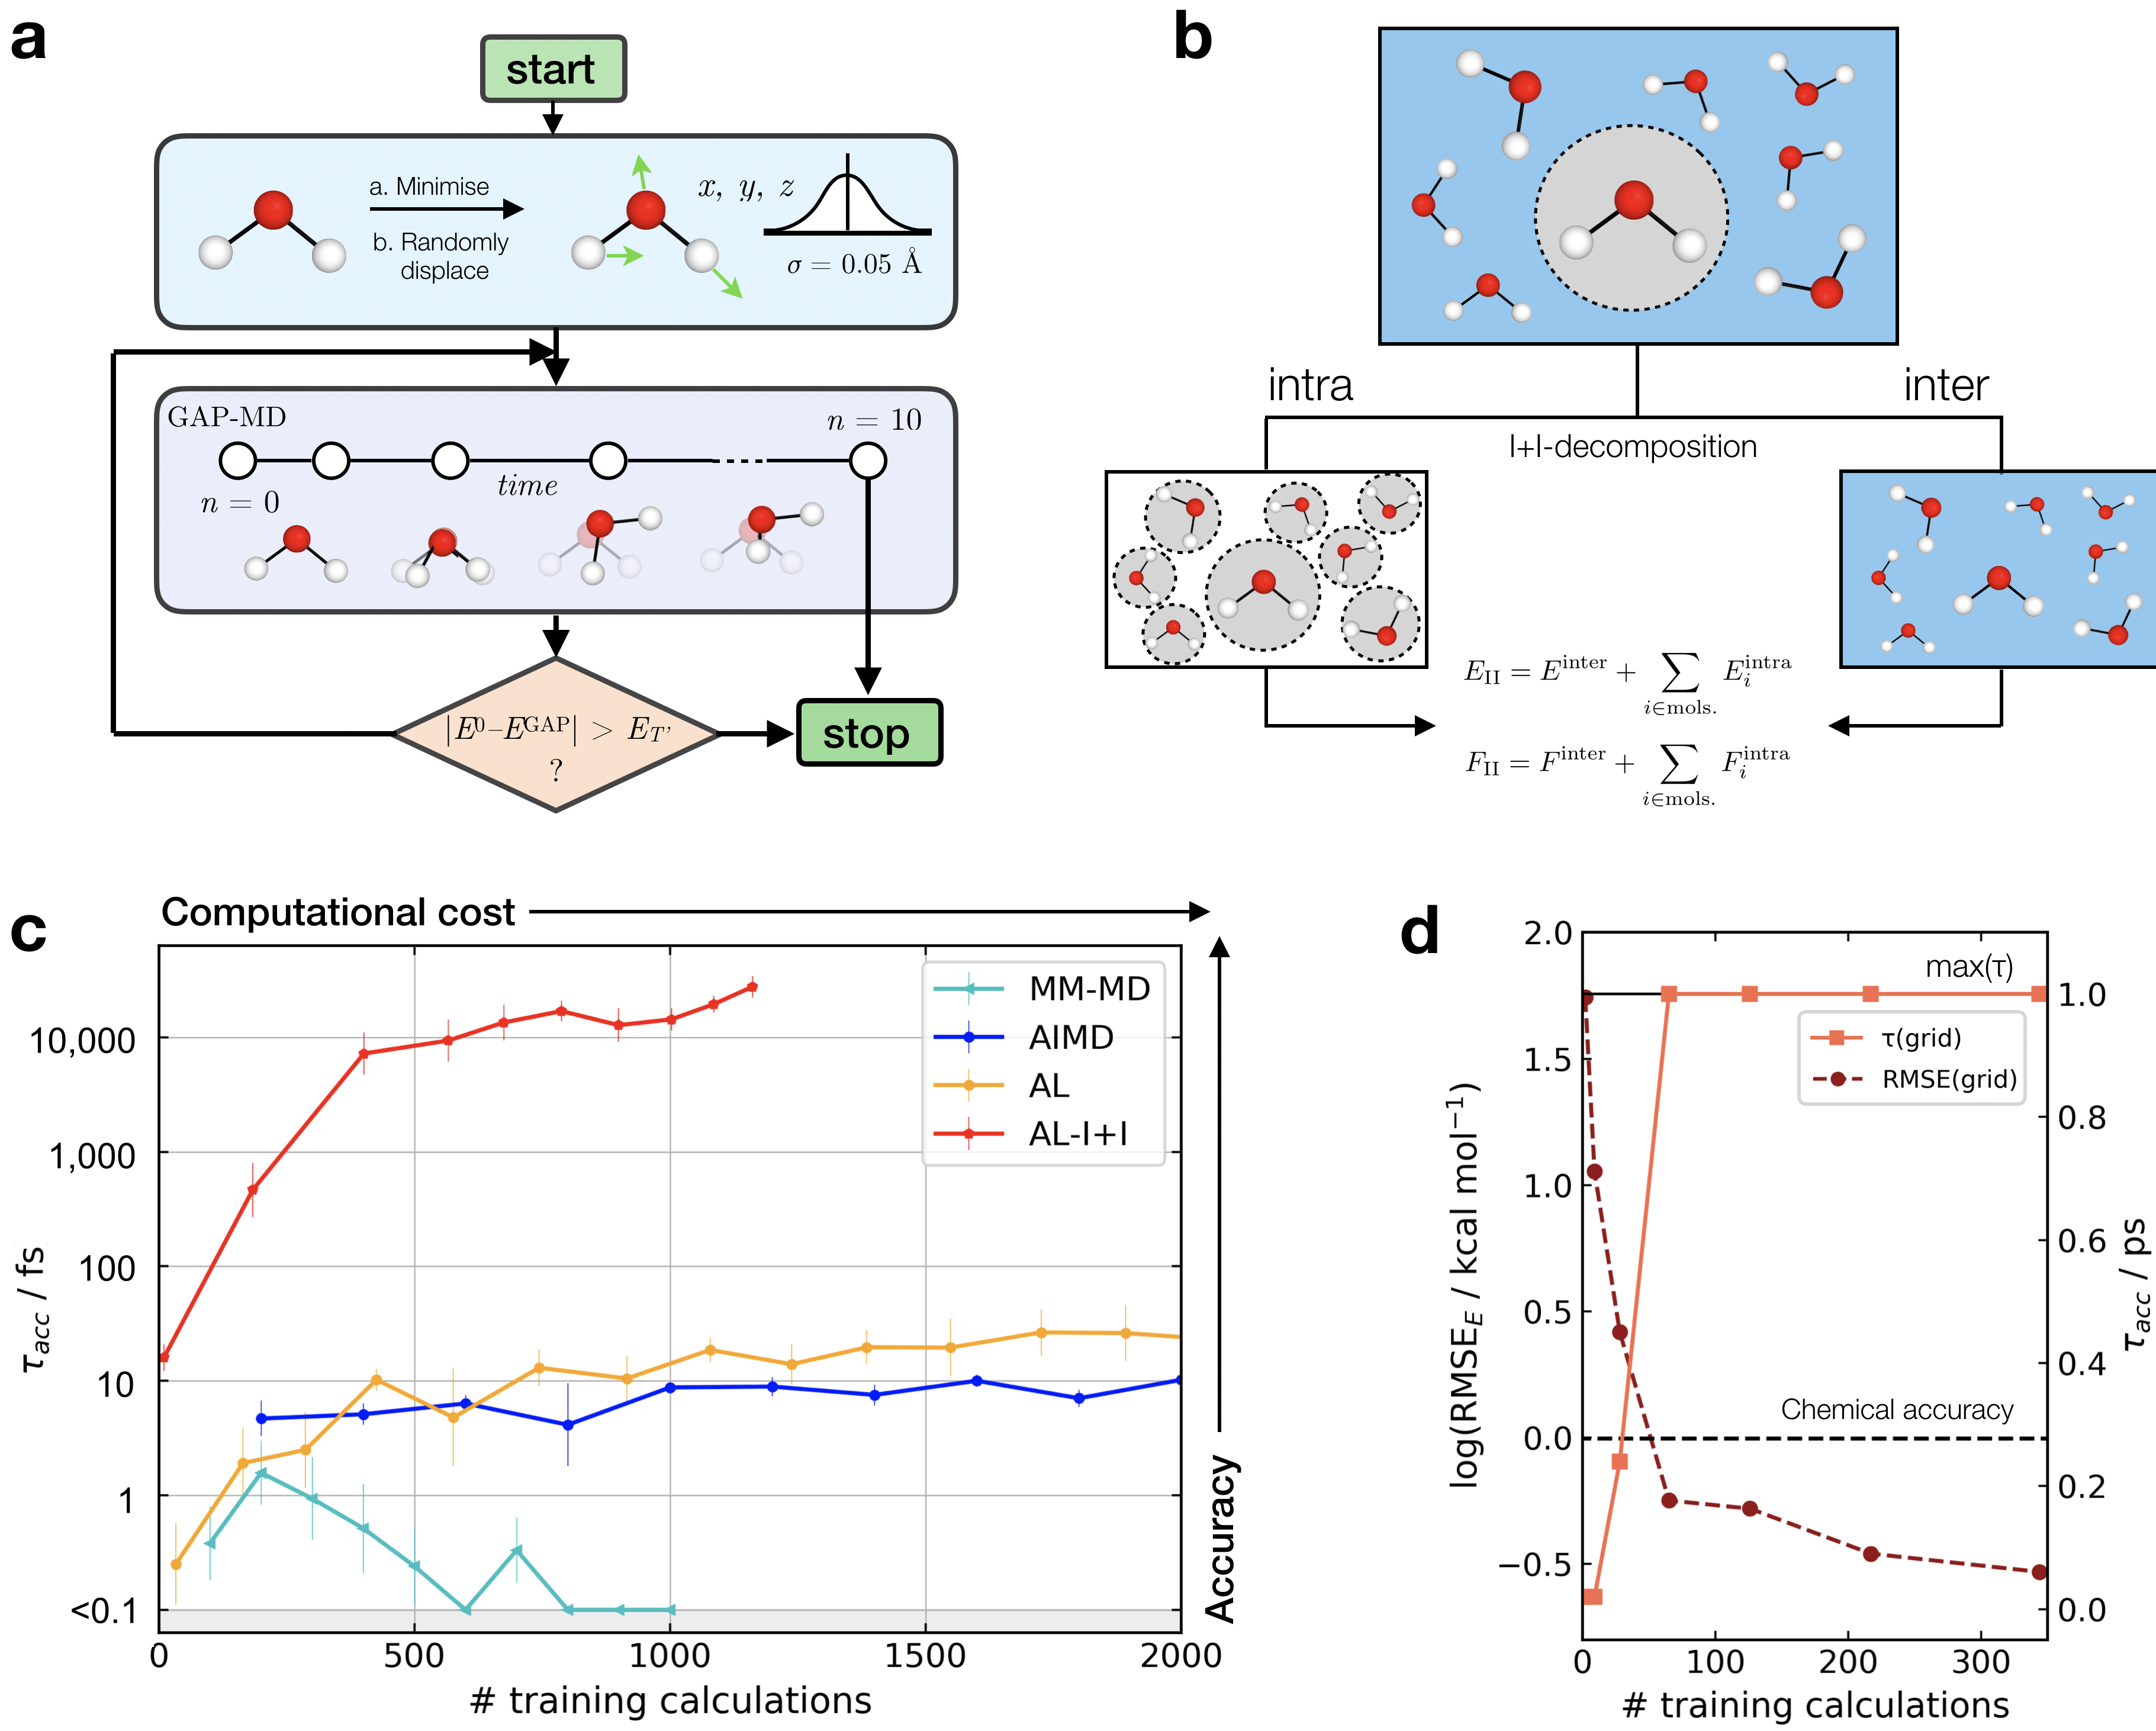
\includegraphics[width=\textwidth]{6/gap/figs_ms/fig1}
	\vspace{0.2cm}
	\hrule
	\caption{Active learning of machine-learning potentials for liquid water. (a) Schematic of the active learning loop implemented for fitting GAP models, where the GAP-MD exploration is run for $n^3 +2$ femtoseconds, where n (the number of evaluations) is incremented after each time the error is evaluated. (b) Schematic illustrating the separation into inter- and intra-molecular terms (I+I) for a bulk water system; these are described by separate GAP models and then added to give the combined prediction for energies, $E$, and forces, $F$. (c) Learning curves for a bulk water GAP model using different training strategies. \taua with $E_l$ = 0.1 eV, $E_T$ = 1 eV, 10 fs interval, 300 K, from the same random minimised configuration of 10 waters in a 7 \AA cubic box. Error bars quoted as the standard errors in the mean from 5 independent repeats. The horizontal axis denotes the number of evaluations in training data generation. See Tables \ref{table::ml_si_1}--\ref{table::ml_si_2} for detailed methods. DFTB(3ob) ground truth. Minimum \taua is shown as 0.1 fs to enable plotting on a log scale. (d) Water monomer model training performance as characterised by \taua and RMSE over the full 3D PES; see Figure \ref{fig::ml_si_2} for details.}
	\label{fig::ml_1}
\end{figure}


We initially employed training strategies found to work well in elemental materials by, for example, fitting a combined potential with two- and three-body GAPs. However, this approach was found to be detrimental to the potential’s stability. This can be understood considering a water dimer (HO–H${}_c \cdots$OH${}_2$); here, a two-body description that treats the two O–H${}_c$ interactions on the same footing is a poor approximation, in view of the different order of magnitude between the interactions at their respective minima (Figure \ref{fig::ml_si_3}). Therefore, we decided to proceed employing a smooth overlap of atomic positions\cite{Bartok2013} (SOAP) descriptor for an exclusively many–body description of atomic environments (with the exception of AL-I+I, which uses 2+3 body for the intramolecular component as discussed later). 

We also explored different approaches to generate the database and their influence on the generated potential. An emerging approach to generate training data for elemental GAPs is to initialise the database with randomised configurations (with reasonable constraints, as in ab initio random structure searching\cite{Pickard2011}), and to gradually explore configuration space with evolving versions of the potential (see, e.g., ref. \cite{Bernstein2019}). However, randomly placing water molecules does not in itself afford a stable potential. A similar result is observed when the most diverse configurations are selected using the CUR algorithm\cite{Mahoney2009, Bernstein2019} (Figure \ref{fig::ml_si_4}) or when applying intramolecular displacements, following minimisation (Figure \ref{fig::ml_si_4}). Selecting frames from classical MD simulations at temperatures of 100–1000 K was also found to be an ineffective strategy (Figure \ref{fig::ml_si_5}), reaching \taua of only a few fs (“MM-MD”, Figure \ref{fig::ml_1}c). This is in line with the results reported in ref. \cite{Cole2020}. Note that this is not because the GAP cannot fit reference energies and forces from
MM configurations (Figure \ref{fig::ml_si_6}), but because of a poor configuration space overlap with the ground truth PES (Figure \ref{fig::ml_si_7}). Selecting configurations from an AIMD simulation at 300 K (AIMD, Figure \ref{fig::ml_1}c) was an improvement over training on random and MM-generated configurations, with \taua $~10$ fs. However, by adding additional AIMD configurations the increase in accuracy saturates quickly even if those are obtained at higher temperatures (Figure \ref{fig::ml_si_8}). Using AIMD configurations can also involve a significant cost (requiring thousands of evaluations). Finally, active learning from only a few randomly generated configurations provides a modest uplift in accuracy (AL, Figure \ref{fig::ml_1}c), with accuracy on-par with GAP trained on AIMD configurations at a third of the required reference data.

Only when the relevant length and energy scales of the system are decomposed by treating intra- and inter-molecular components separately (Figure \ref{fig::ml_1}b) a potential that is stable for picoseconds is obtained (AL-I+I, Figure \ref{fig::ml_1}c). We note that this approach is related to the hierarchical fitting of GAPs\cite{Veit2019, Bartok2013} and related ML models\cite{Dral2020, Ramakrishnan2015, Schran2020, Sukuba2018} using different levels of computational approaches, and the decomposition strategy by Wengert and co-workers.\cite{Wengert2021} In the present work, we employ the same ground-truth method throughout rather than combining different levels of theory for the input data, but as in prior studies we describe the stronger (e.g., covalent) and weaker intermolecular terms with separate fits that are afterwards combined to give the final model. The intramolecular GAP for water contains only 2- and 3-body terms and the training data are chosen using an evenly spaced grid over the full 3-atom PES ($8\times8\times8$ grid points in $r_\text{OH}$ and $r_\text{HH}$, $\sim$0.1 \AA$\;$ spacing, Figure \ref{fig::ml_si_9}). Energy and force evaluations of this potential are a simple sum of intra- and inter-molecular terms, but require the former to be evaluated in an expanded simulation box to ensure no non-bonded hydrogen atoms are present within the cut-off radius of the 2- and 3-body descriptors on oxygen (Figure \ref{fig::ml_si_10}). Here the intramolecular PES is fairly low-dimensional, so a full and reasonably dense grid is available, which in turn allows us to define an error measure over the whole PES, where we find the error to be inversely correlated with \taua (Figure \ref{fig::ml_1}d). Using an acceptable error of 0.2 \kcalx per H${}_2$O molecule for a description of bulk water, which is similar to that achieved in a recent NN fit of water,\cite{Cheng2019} we find that this potential affords \taua $>10$ ps with just a few hundred ground truth evaluations (AL-I+I, Figure \ref{fig::ml_1}c). To put this value in context, we measured \taua for the fully reactive water NN of Cheng et al.,\cite{Cheng2019} which was trained on $\sim$7000 reference configurations (DFTB energy/forces) and has shown to provide a highly accurate water model over multiple states. For this state-of-the-art ML potential, a \taua value of 7.6$\pm$0.7 ps for liquid at 300 K is obtained, comparable to the one obtained for the new AL-based potentials of the present work ($>10$ ps). Of course, direct comparison requires caution because the GAP and NN potentials are different in scope: the former employs a large reference database to develop a general water model, whereas the present study targets robust potentials for liquid water with minimal computational effort, in turn allowing the user to apply similar approaches to other chemical systems (as will be shown below). 

The model fitted using our approach (AL-I+I) yields radial distribution functions (RDFs) in good agreement with the ground-truth method, initially chosen to be DFTB, both considering the location and intensities of the peaks corresponding to the first and second coordination shells (Figure \ref{fig::ml_2a-d}a-c). This is despite the relatively short-range atomic cut-offs (3 \AA, O only) used. Only in the O–O pair RDF there is a slight deviation from the DFTB ground truth, precisely where the potential is zero outside the 3 Å cut-off radius of the SOAP descriptor. Interestingly, for a DFT-quality GAP simply re-evaluating energies and forces on DFTB-derived active-learnt configurations is insufficient, with the DFTB configurations being high in energy at the DFT level ($~5$ eV, Figure \ref{fig::ml_si_11}). However, applying an active learning strategy with a PBE reference method and a slightly larger 3.5 \AA cut-off generates excellent agreement with the AIMD simulation from ref. \cite{Zheng2018}, in only a few hours of total training time (Figure \ref{fig::ml_2a-d}d-f). At this level of theory, the local structure of liquid water is predicted largely correctly, with two distinct peaks in the O--H RDF, corresponding to first and second solvation shells with the largest deviation from the ground truth again in the O--O pair around the descriptor cut-off. The real significance, of course, is in moving to more accurate ground-truth methods, for which a full MD would not be straightforward: indeed, using the same method, a hybrid DFT-quality water model can be generated within a few days, which would be inaccessible with other methods (the generation of the GAP model required $~5$ days on 20 CPU cores, Figure \ref{fig::ml_2e-i}g-i). These results suggest that the training strategy (and hyperparameter selection) presented here is suitable independent of the reference method.


\begin{figure}[h!]
	\vspace{0.4cm}
	\centering
	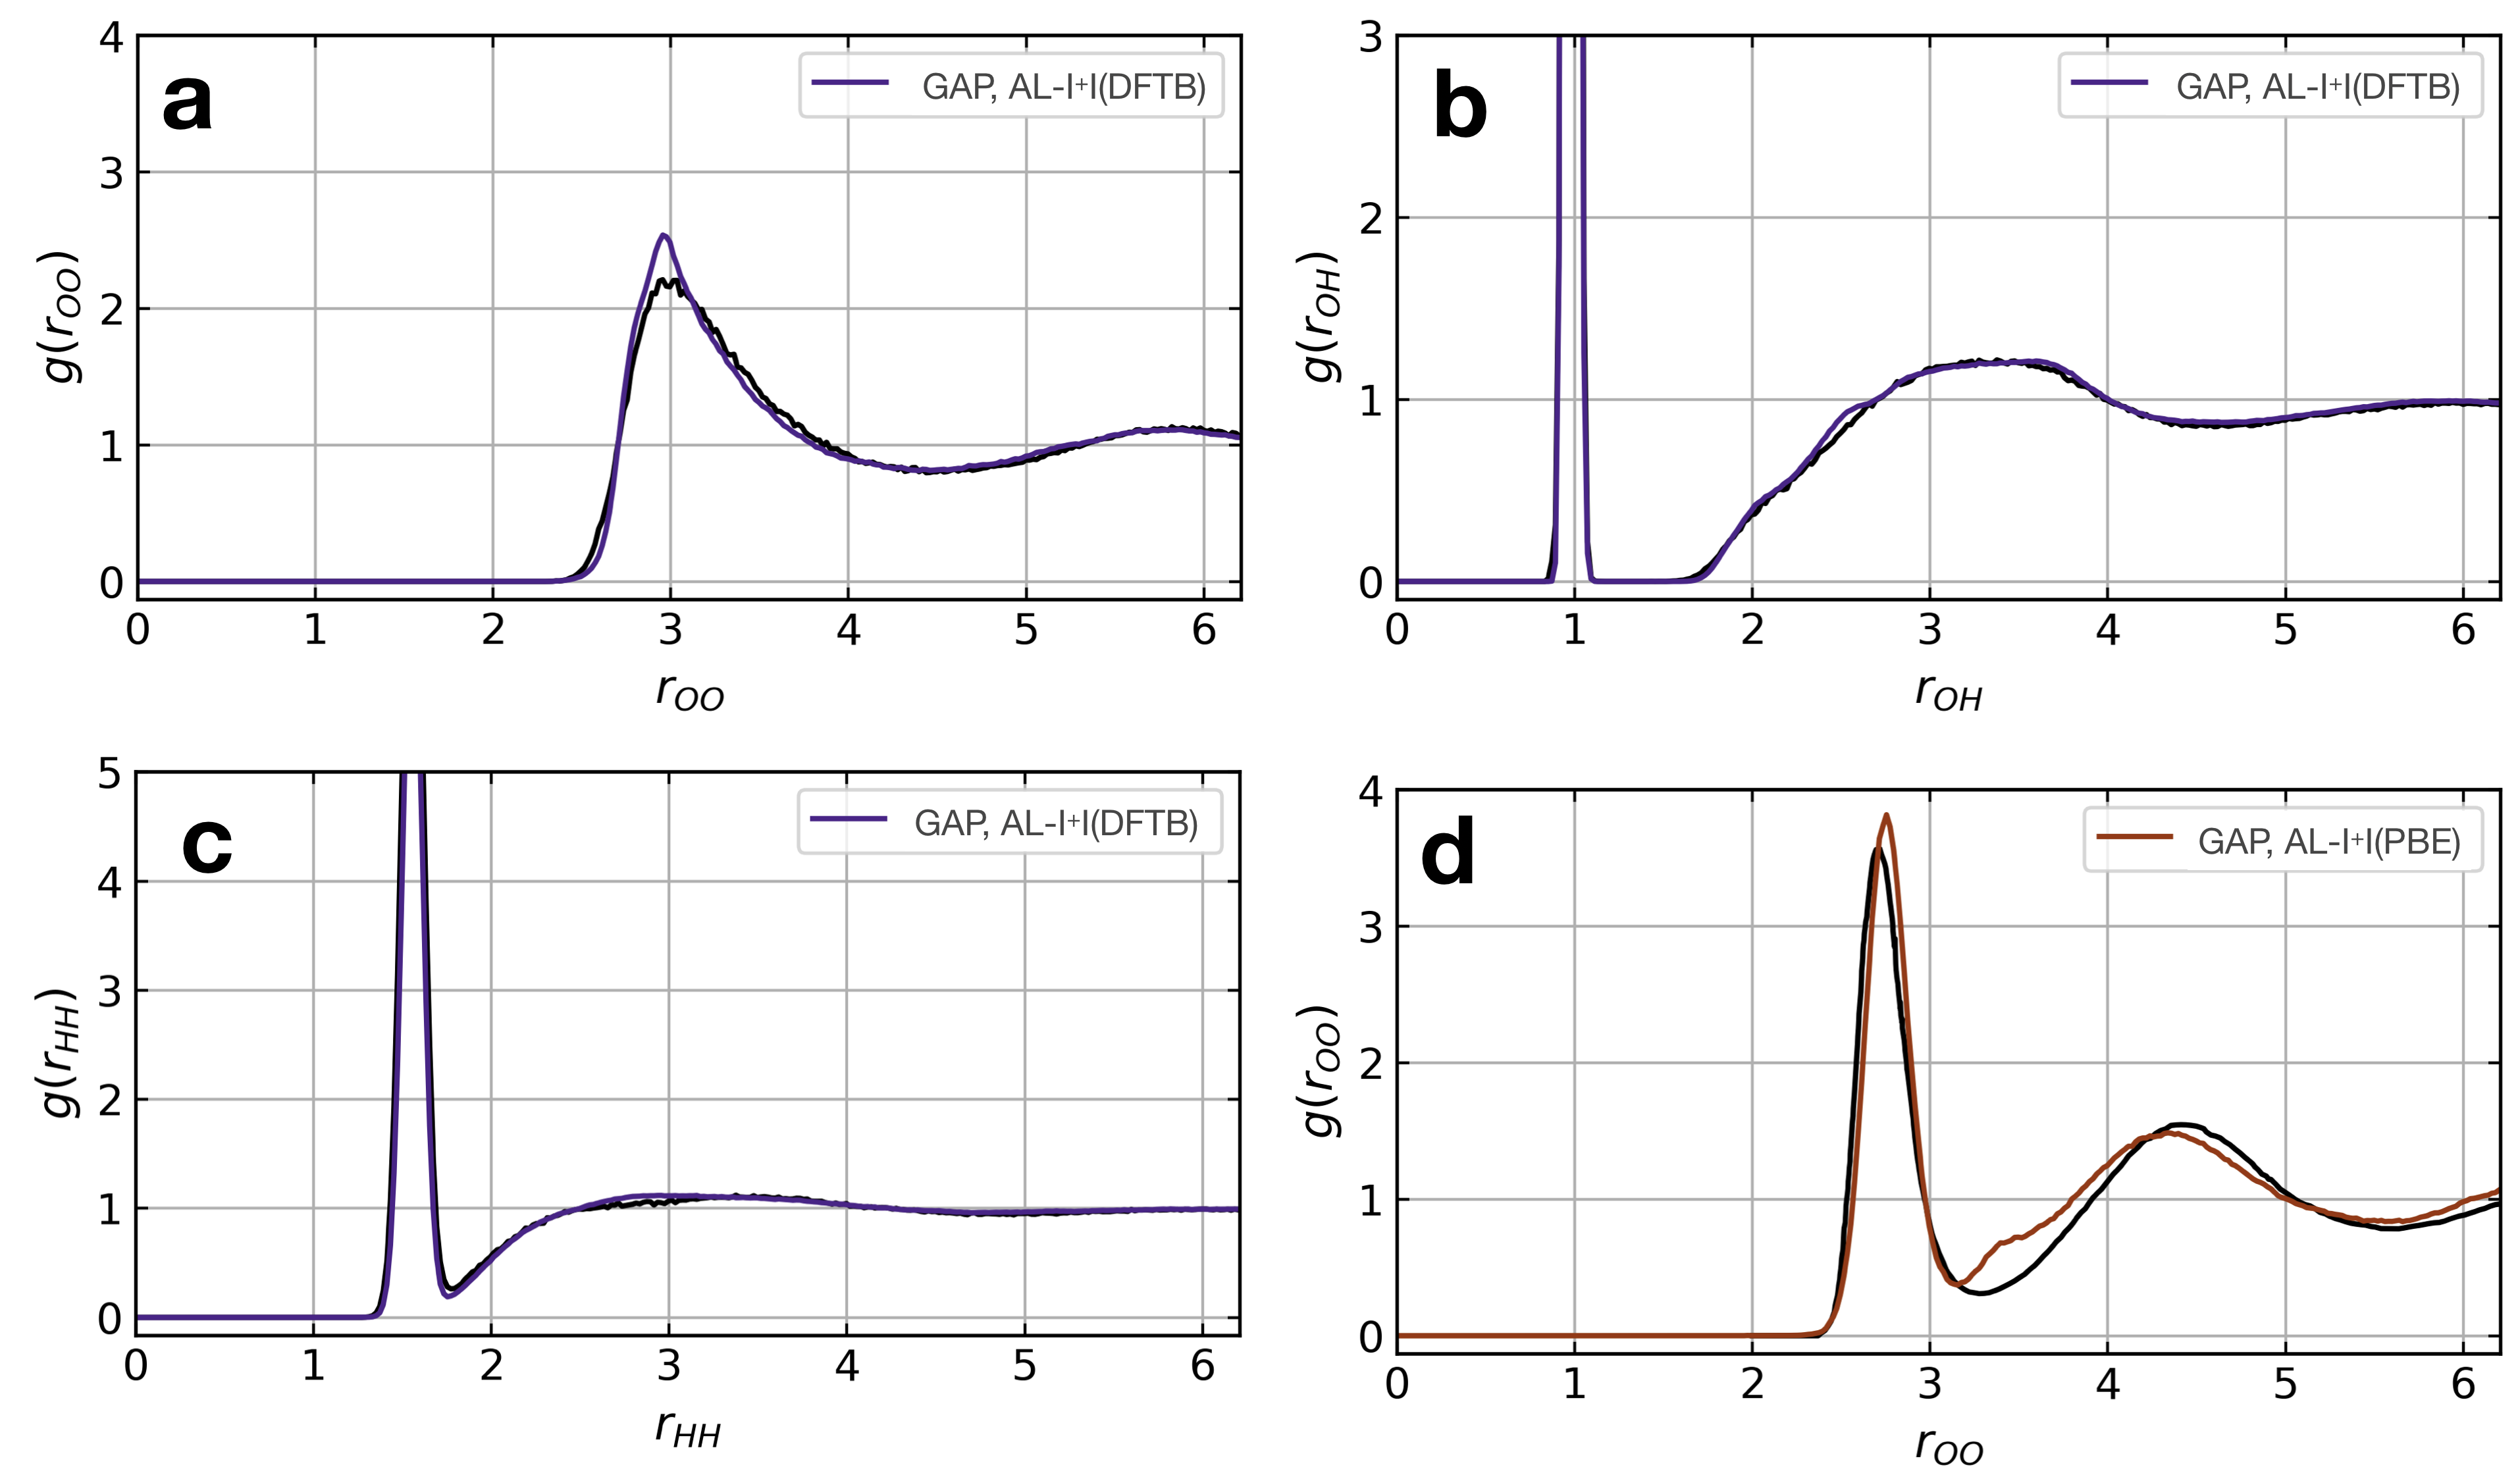
\includegraphics[width=\textwidth]{6/gap/figs_ms/fig2a-d}
	\vspace{0.2cm}
	\hrule
	\caption{Liquid water simulations. Active learning of bulk water models at various levels of theory. Shown here are oxygen–oxygen, oxygen–hydrogen, and hydrogen–hydrogen radial distribution functions from NVT MD simulations of 64 water molecules in a 12.42 \AA cubic box, with ground truth (black) and GAP (purple / red) simulations. (a–c) DFTB(3ob params) ground truth, 100 ps, 300 K, $r_c^\text{SOAP}(O) = 3$ \AA.}
	\label{fig::ml_2a-d}
\end{figure}
\begin{figure}[h!]
	\vspace{0.4cm}
	\centering
	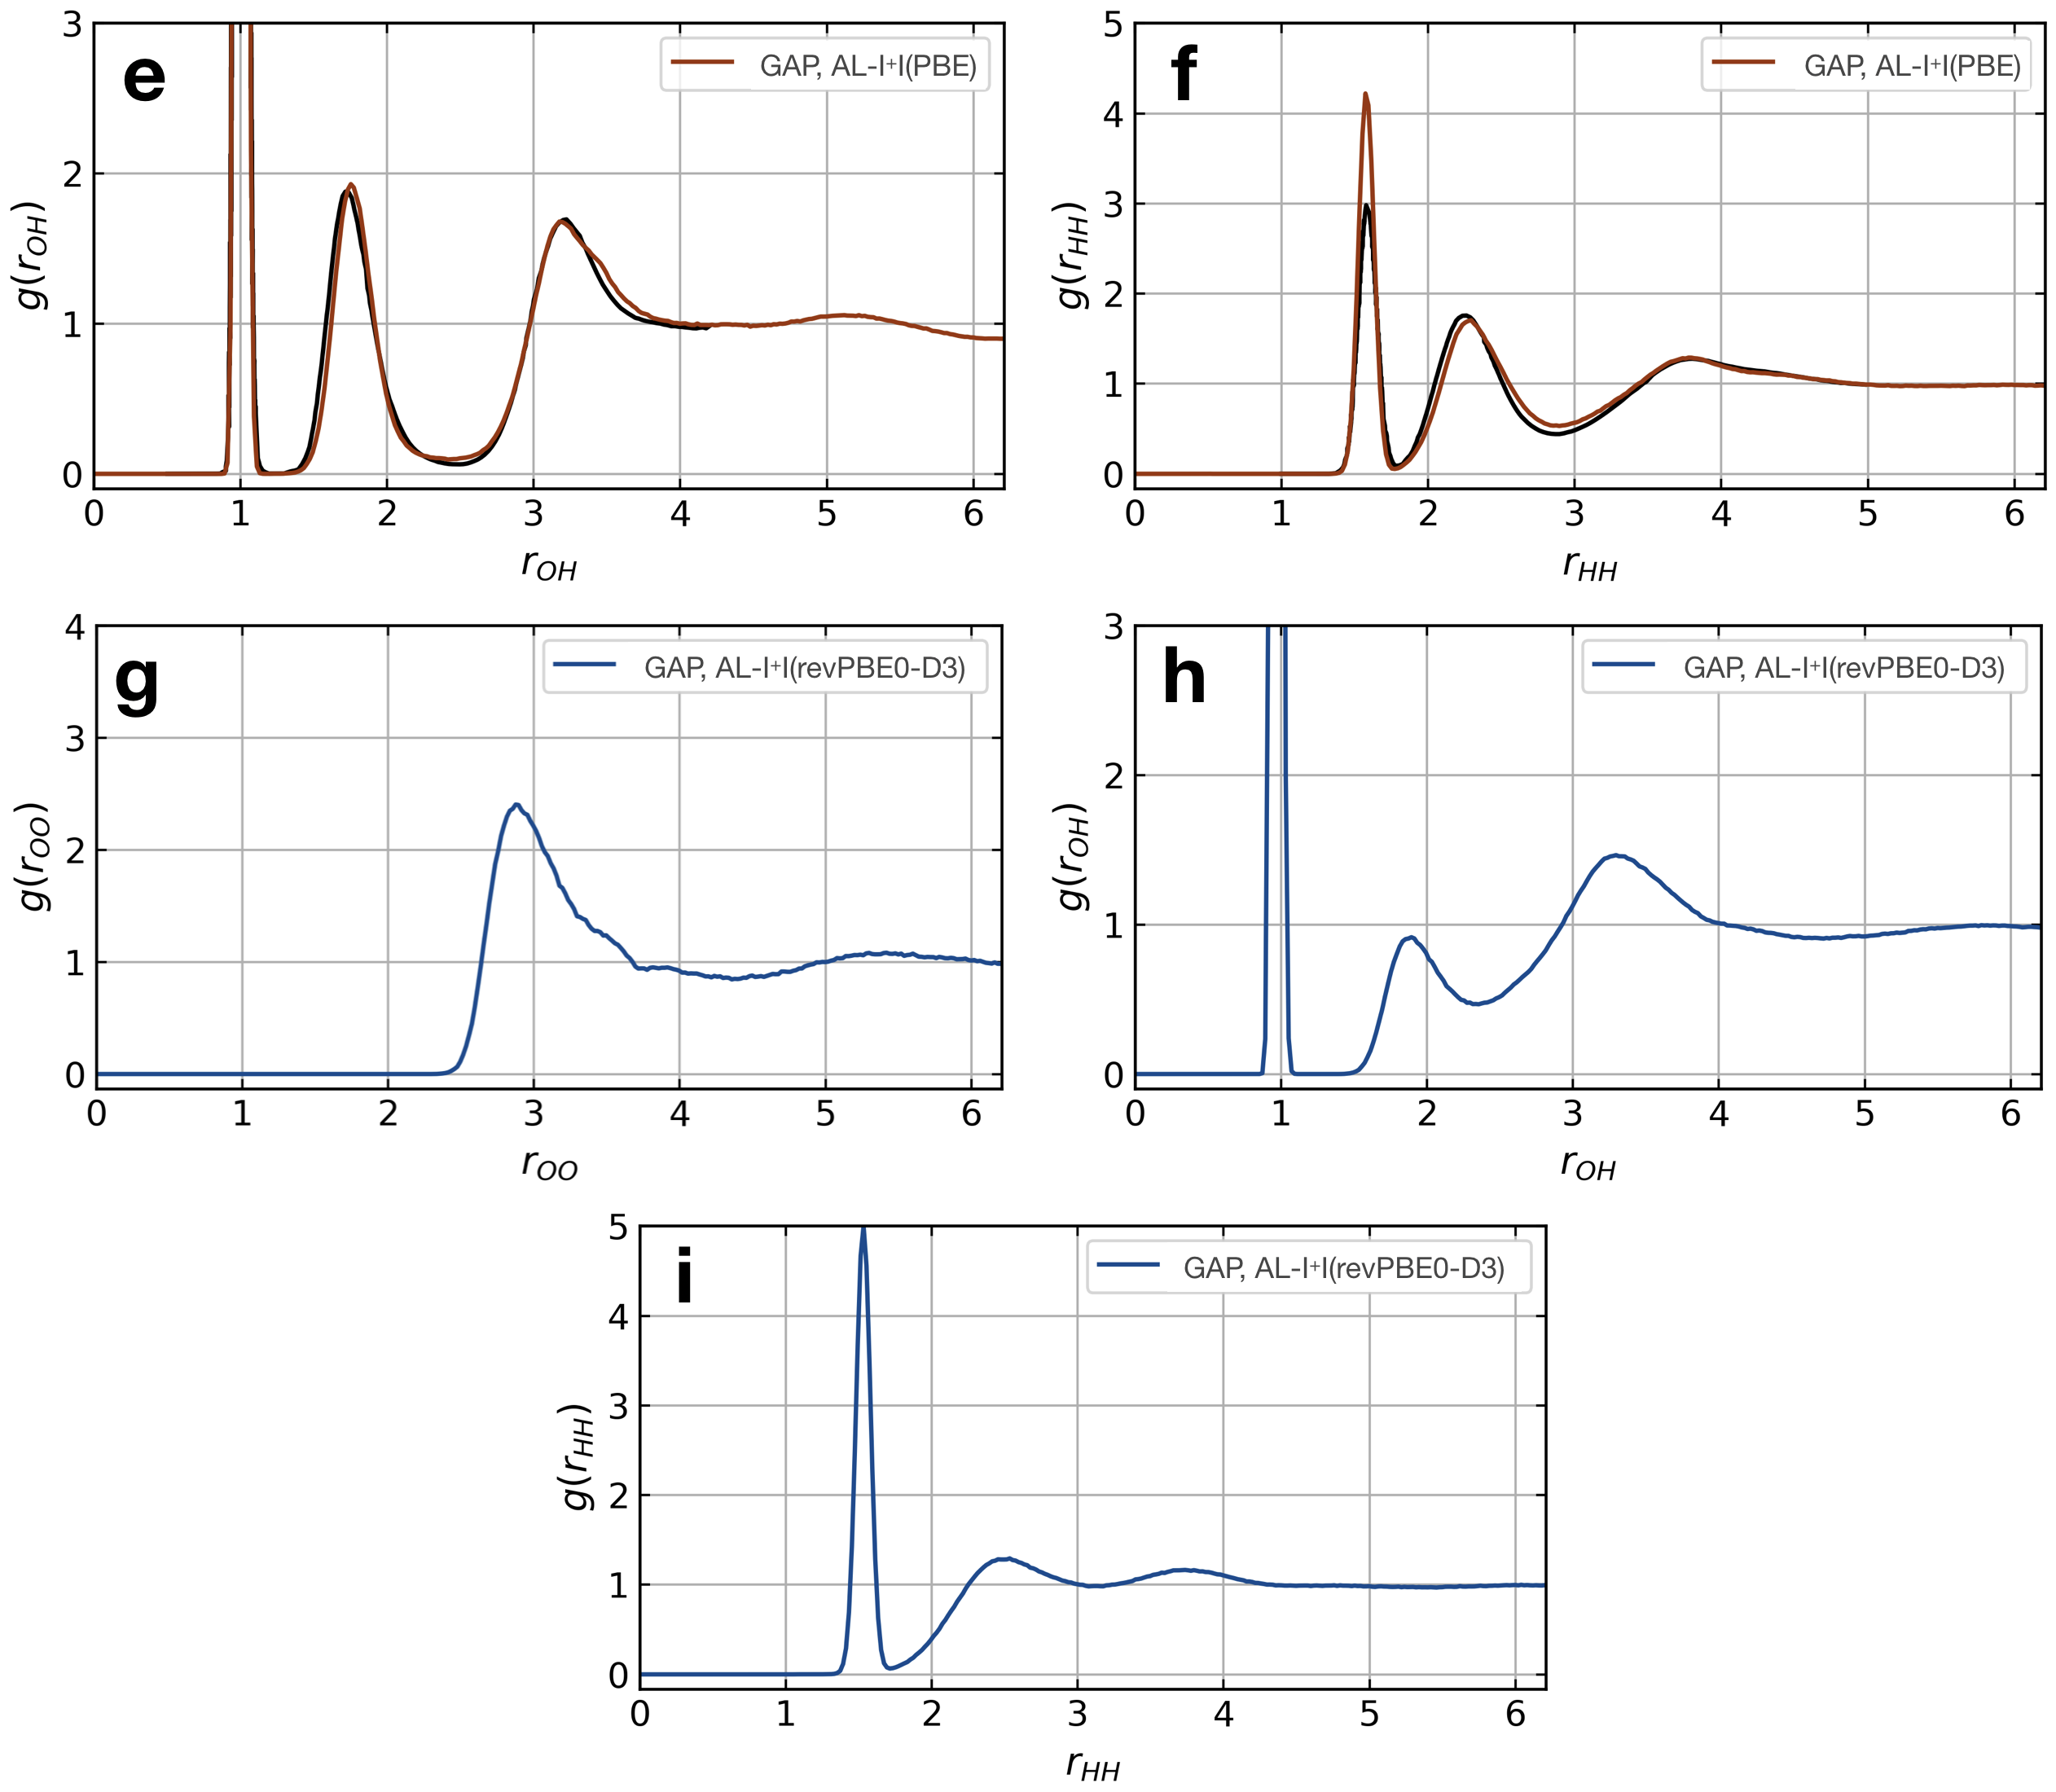
\includegraphics[width=\textwidth]{6/gap/figs_ms/fig2e-i}
	\vspace{0.2cm}
	\hrule
	\caption{Liquid water simulations cont. (e–f) DFT(PBE) reference RDF data extracted from ref. \cite{Zheng2018}, 30 ps, 330 K, $r_c^\text{SOAP}(O) = 3.5$ \AA. (g-i) DFT(revPBE0-D3) GAP, 30 ps, 330 K, $r_c^\text{SOAP}(O) = 4.0$ \AA.}
	\label{fig::ml_2e-i}
\end{figure}

\clearpage

\subsubsection{Other Solvent Systems}
Organic reactions often take place in solvents other than water. Using an identical training strategy to the one described for water, we trained GAPs for a selection of organic solvents with various types of intermolecular interactions. To quickly generate the reference simulation data for this proof-of-concept, a DFTB ground truth is employed; chlorinated solvents were not selected due to a large discrepancy between the DFTB-generated and experimental C–Cl bond dissociation energy (Figure \ref{fig::ml_si_12}). A uniform grid over the intramolecular PES is now no longer possible; thus, AL is used to develop an initial intramolecular potential trained using GAP-MD at 1600 K (Figure \ref{fig::ml_si_13}). This temperature is used to sample higher-energy configurations more efficiently. In all cases, only hundreds of ground truth evaluations were necessary to generate GAPs affording stable dynamics, with \taua values on the order of picoseconds (Figure \ref{fig::ml_si_14}, Table \ref{table::ml_1}). 


\begin{table}[h!]
	\def\arraystretch{1.5}
	\begin{tabularx}{\textwidth}{YYYY}
		\hline
		Solvent &SOAP on  & $N_\text{intra}$	& $N_\text{inter}$\\
		\hline
	
		Acetonitrile &	C, N &	269$\pm$12	 &120$\pm$60
\\
		Methanol &  	C, O &	221$\pm$13	 &292$\pm$49
\\
		Acetone &	  C, O &	566$\pm$80	 &359$\pm$29
\\
		Pyridine &   	C, N &	249$\pm$36 &	243$\pm$11
\\
		Ammonia	 &  N	   &38$\pm$40	 &109$\pm$24
	\\
		\hline
	\end{tabularx}

	\caption{Average number ($N$) of total ground truth evaluations (over 5 repeats quoted with a standard error in the mean) required to obtain a potential with \taua $>$ 3 ps, where $E_T$ = 1 eV, $E_l$ = 0.1 eV, 300 K. All SOAP descriptors used 3.0 \AA$\;$ cut–offs; they are centred on the stated atomic species, and include all atoms within the neighbourhood of those atoms (including hydrogen).}
	\label{table::ml_1}
\end{table}


For a representative example, the computed RDFs for acetonitrile compare well with the ground truth (Figure \ref{fig::ml_si_15}). As with the water models above, to quantitatively evaluate bulk properties training an accurate reference method and the inclusion of nuclear quantum effects would be necessary.\cite{Veit2019, Cheng2019} Nevertheless, this example demonstrates that the training method is applicable to a range of chemical systems beyond water. 

\subsubsection{Aqueous Zn(II)}

Modelling metal ions in solution remains one of the main challenges for general-purpose force fields.\cite{Li2017chemrev} Historically, metal centres have been developed by fitting van der Waals parameters to reproduce RDFs and hydration free energies of aquo complexes, which are expected to be transferable to more chemically complex environments. However, while simple, these models have often led to unstable simulations or poorly describe structural properties.\cite{Li2017chemrev} Considering these challenges and their relevance in biomolecular modelling, we decided to use our strategy to generate a GAP for aqueous Zn(II) ion as a representative system. Here the system was decomposed into a [Zn(H${}_2$O)${}_6$]${}^{2+}$ cluster and the remaining water molecules. A strategy identical to the one described for water was used, training the intermolecular interactions separately with a 4.0 \AA intermolecular cut-off for the oxygen atoms. Using this potential, MD simulations were propagated at 300 K reproducing the experimental\cite{Ohtaki1993} coordination number (CN=6), and Zn--O distances of both the first (2.08 \AA) and second hydration shells without further optimisation (Figure \ref{fig::ml_3}).

The accuracy of the local structure compared to experiment in the first and second solvation shell indicates that this partitioning is effective at capturing both strong dative M–OH${}_2$ interactions and weaker hydrogen bonding effects. From random points in the configuration space of [Zn(H${}_2$O)${}_6$]${}^{2+}$ and 20 water molecules (intermolecular distances $> 1.7$ \AA, 10 \AA$\;$ cubic box), \taua reached 0.5 ps ($E_l$ = 0.8 \kcalx per H${}_2$O, 20 fs interval). Note this value is far short of the 100 ps simulations performed to generate the RDF and illustrates that a potential may be ‘stable’ and not sample any high energy regions for $t \gg \tau_\text{acc}$. Here, the potential for the Zn-water cluster was trained on almost 1000 configurations, suggesting that tens of atoms per component may be the upper limit in dimensionality for which a model can be trained within a day.

\begin{figure}[h!]
	\vspace{0.4cm}
	\centering
	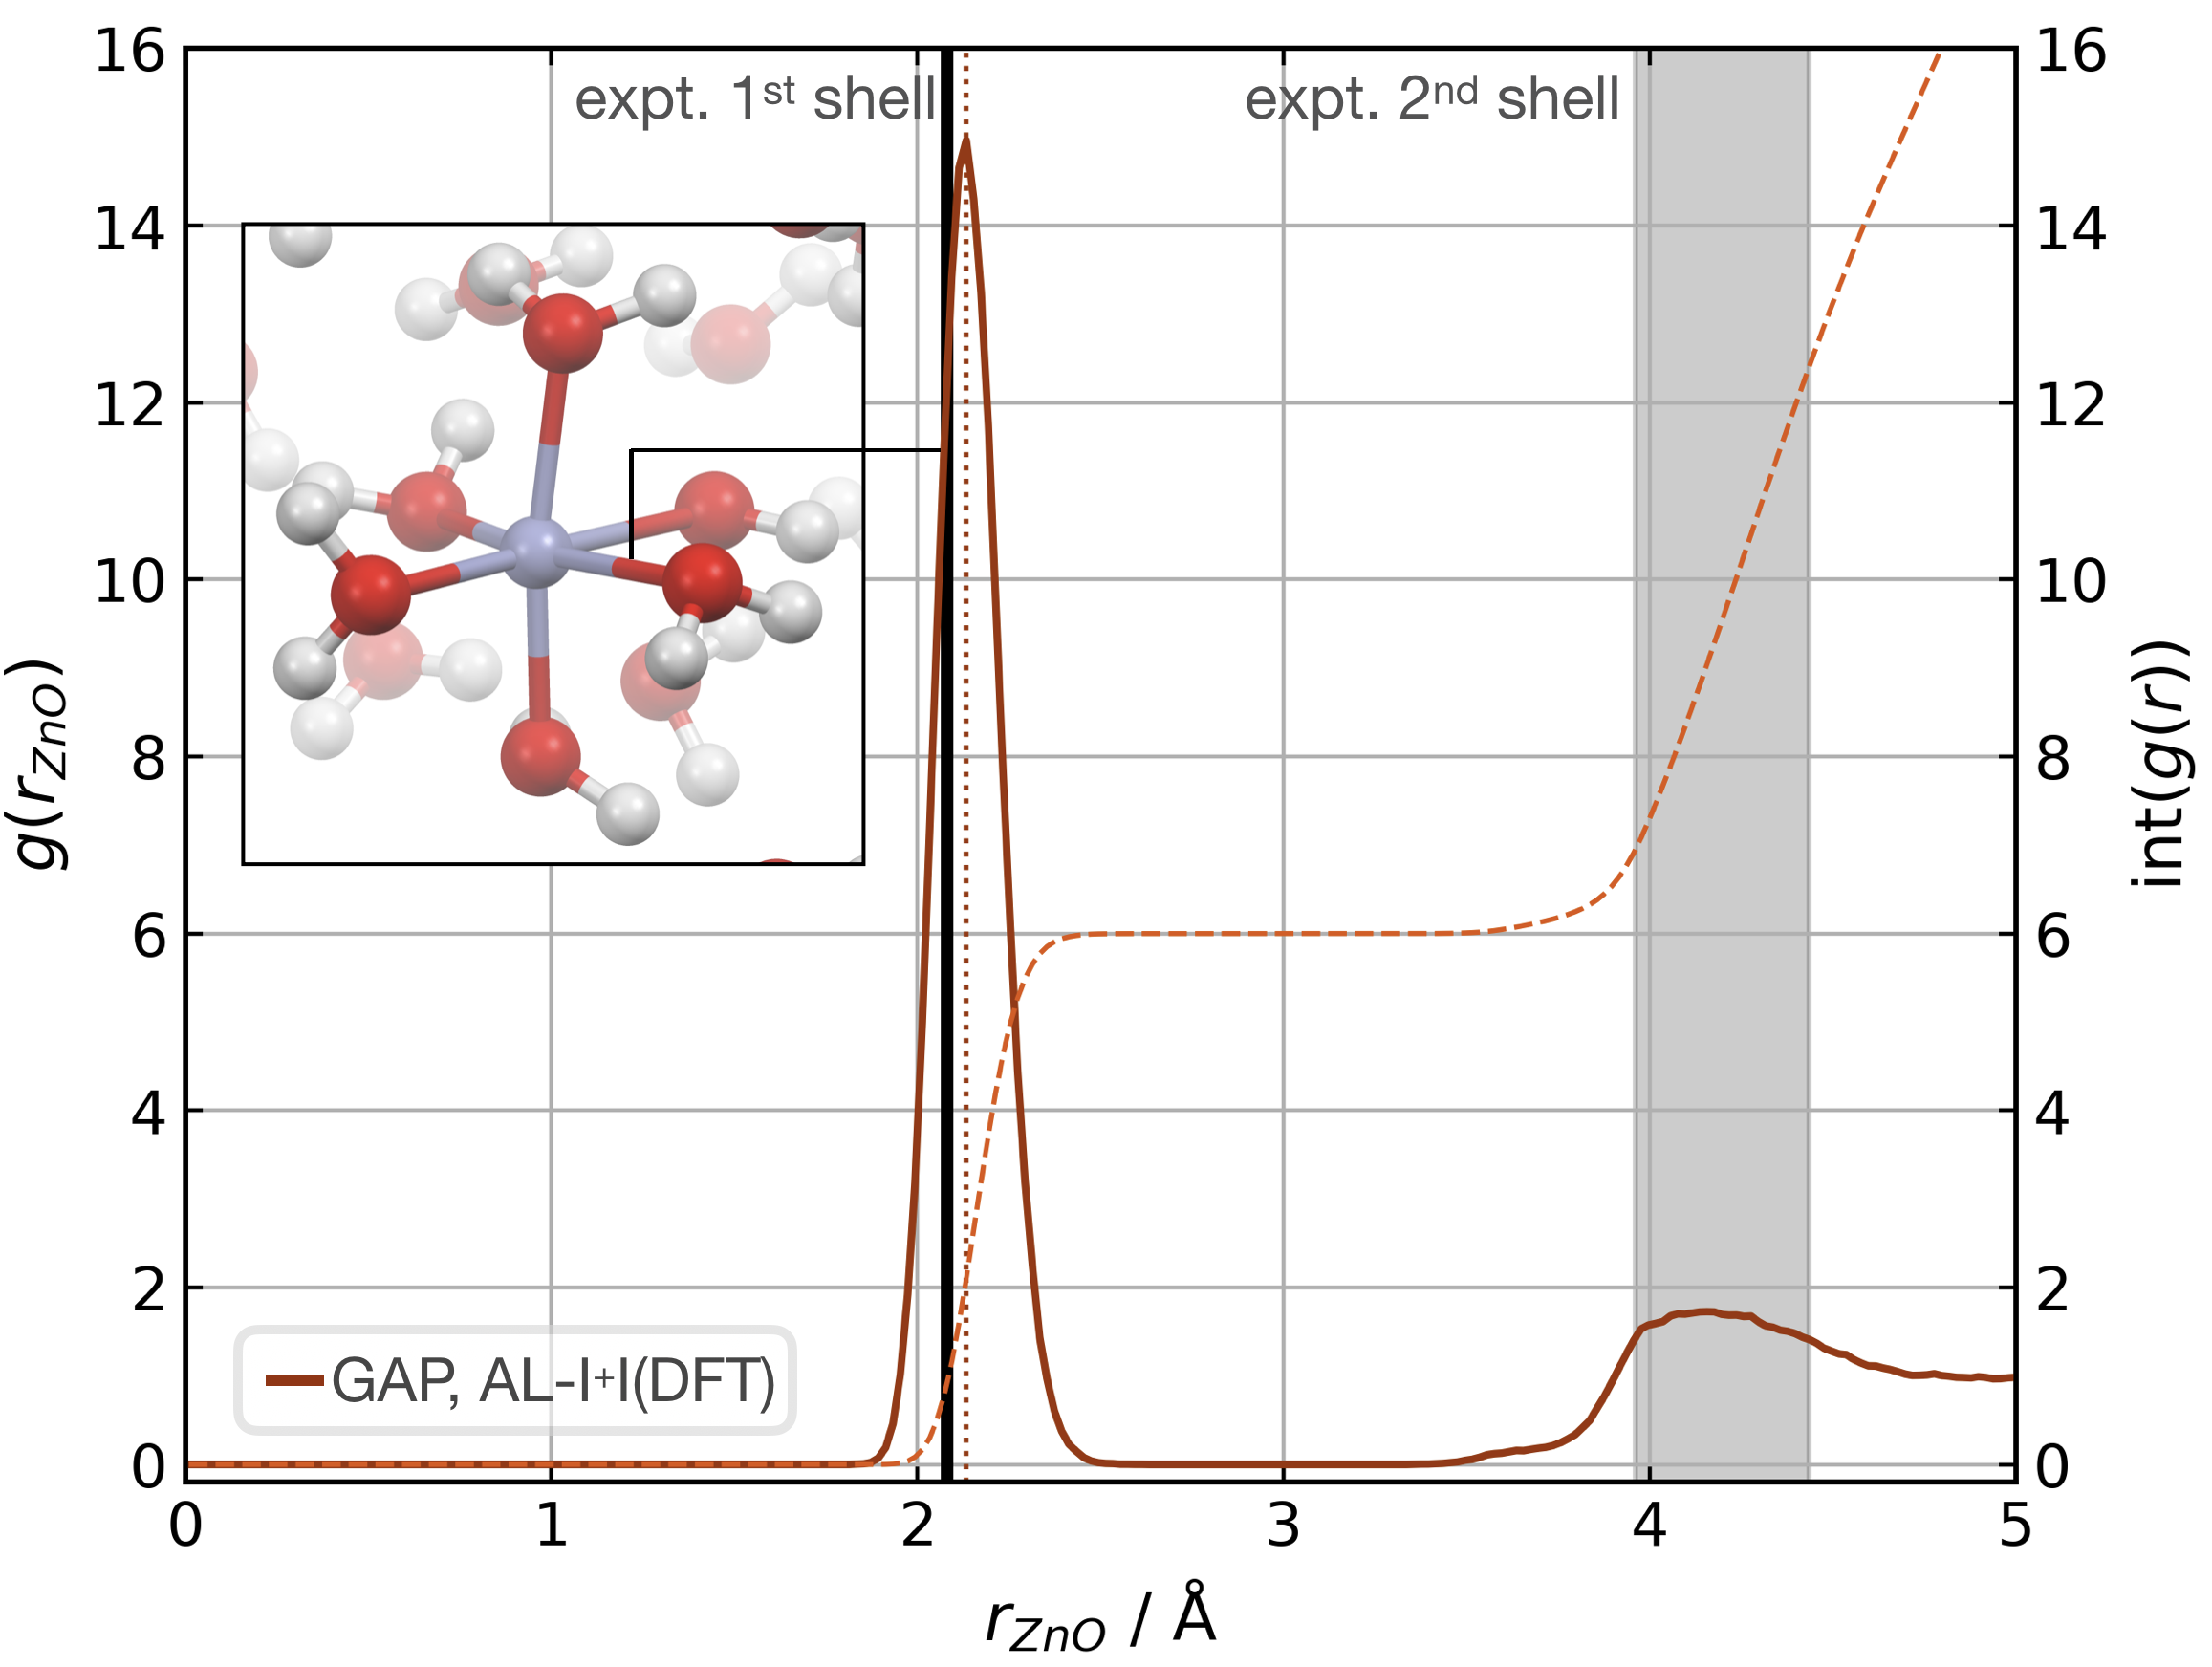
\includegraphics[width=11cm]{6/gap/figs_ms/fig3}
	\vspace{0.2cm}
	\hrule
	\caption{Zn(aq) simulation. Zn–O radial distribution function averaged from 1 ns of cumulative (10 × 100 ps) NVT MD simulations of Zn(II) in aqueous solution at 300 K, with the experimental modal Zn–O distance shown in black. Experimental (X-ray diffraction) Zn–O distances from ref. \cite{Ohtaki1993}, octahedral first hydration shell. Shaded area denotes the range of experimental second hydration shell (ref. \cite{Ohtaki1993} and cited within). GAP trained as those in Table 1 using a PBE/400 eV ground truth, intra-Zn(H${}_2$O)${}_6$ used a O SOAP $r_c = 3.0$ \AA$\;$ and inter $r_c = 4.0$ \AA.}
	\label{fig::ml_3}
\end{figure}


\subsubsection{Metallocage Dynamics}

With a method capable of generating high-quality potentials for modestly sized chemical systems, we next demonstrate the applicability of the strategy to investigate a supramolecular metallocage consisting of $>$100 atoms including metal ions. As a representative example, we selected the [Pd${}_2$L${}_4$]$^{4+}$ metallocage architecture (L = organic pyridine-based ligand), which occupies a prominent place in supramolecular chemistry. Previously, we have studied this system due to its catalytic proficiency in Diels-Alder reactions employing both classical and DFT modelling.\cite{Young2019} The different flexibility of two similar cage architectures was found to be key in explaining their contrasting catalytic activity. 
Taking advantage of the symmetry in the system, a representative fragment containing one full ligand and three pyridine molecules coordinated to a Pd(II) metal ion (68 atoms) was used to fit a GAP for the entire cage (138 atoms) in the gas phase. This potential was trained in a few days ($\sim$1400 CPUh). We used the resulting GAP to perform nanosecond MD simulations on the whole metallocage at 300 K in the gas phase. This simulation took one day and $\sim$100 CPUh to complete. For comparison, an equivalent AIMD simulation would take around 50 years with the reference level of theory employed here. The
flexibility of the system was monitored and compared to the one obtained using classical MD simulations in dichloromethane solvent.\cite{Young2019} Compared to classical MD simulations, using helicity as a measure of flexibility, our potential describes the cage as being more rigid; this suggests that the classical potential overestimates the dynamic flexibility (Figure \ref{fig::ml_4}). This difference is expected as the classical potential has no C-C$\equiv$C-C dihedral barrier, which is presumably correctly captured in the GAP. This example illustrates the general applicability of the approach to increasingly complex systems, where the training of a simpler but representative fragment is sufficient to capture the relevant features of the full system.



\begin{figure}[h!]
	\vspace{0.4cm}
	\centering
	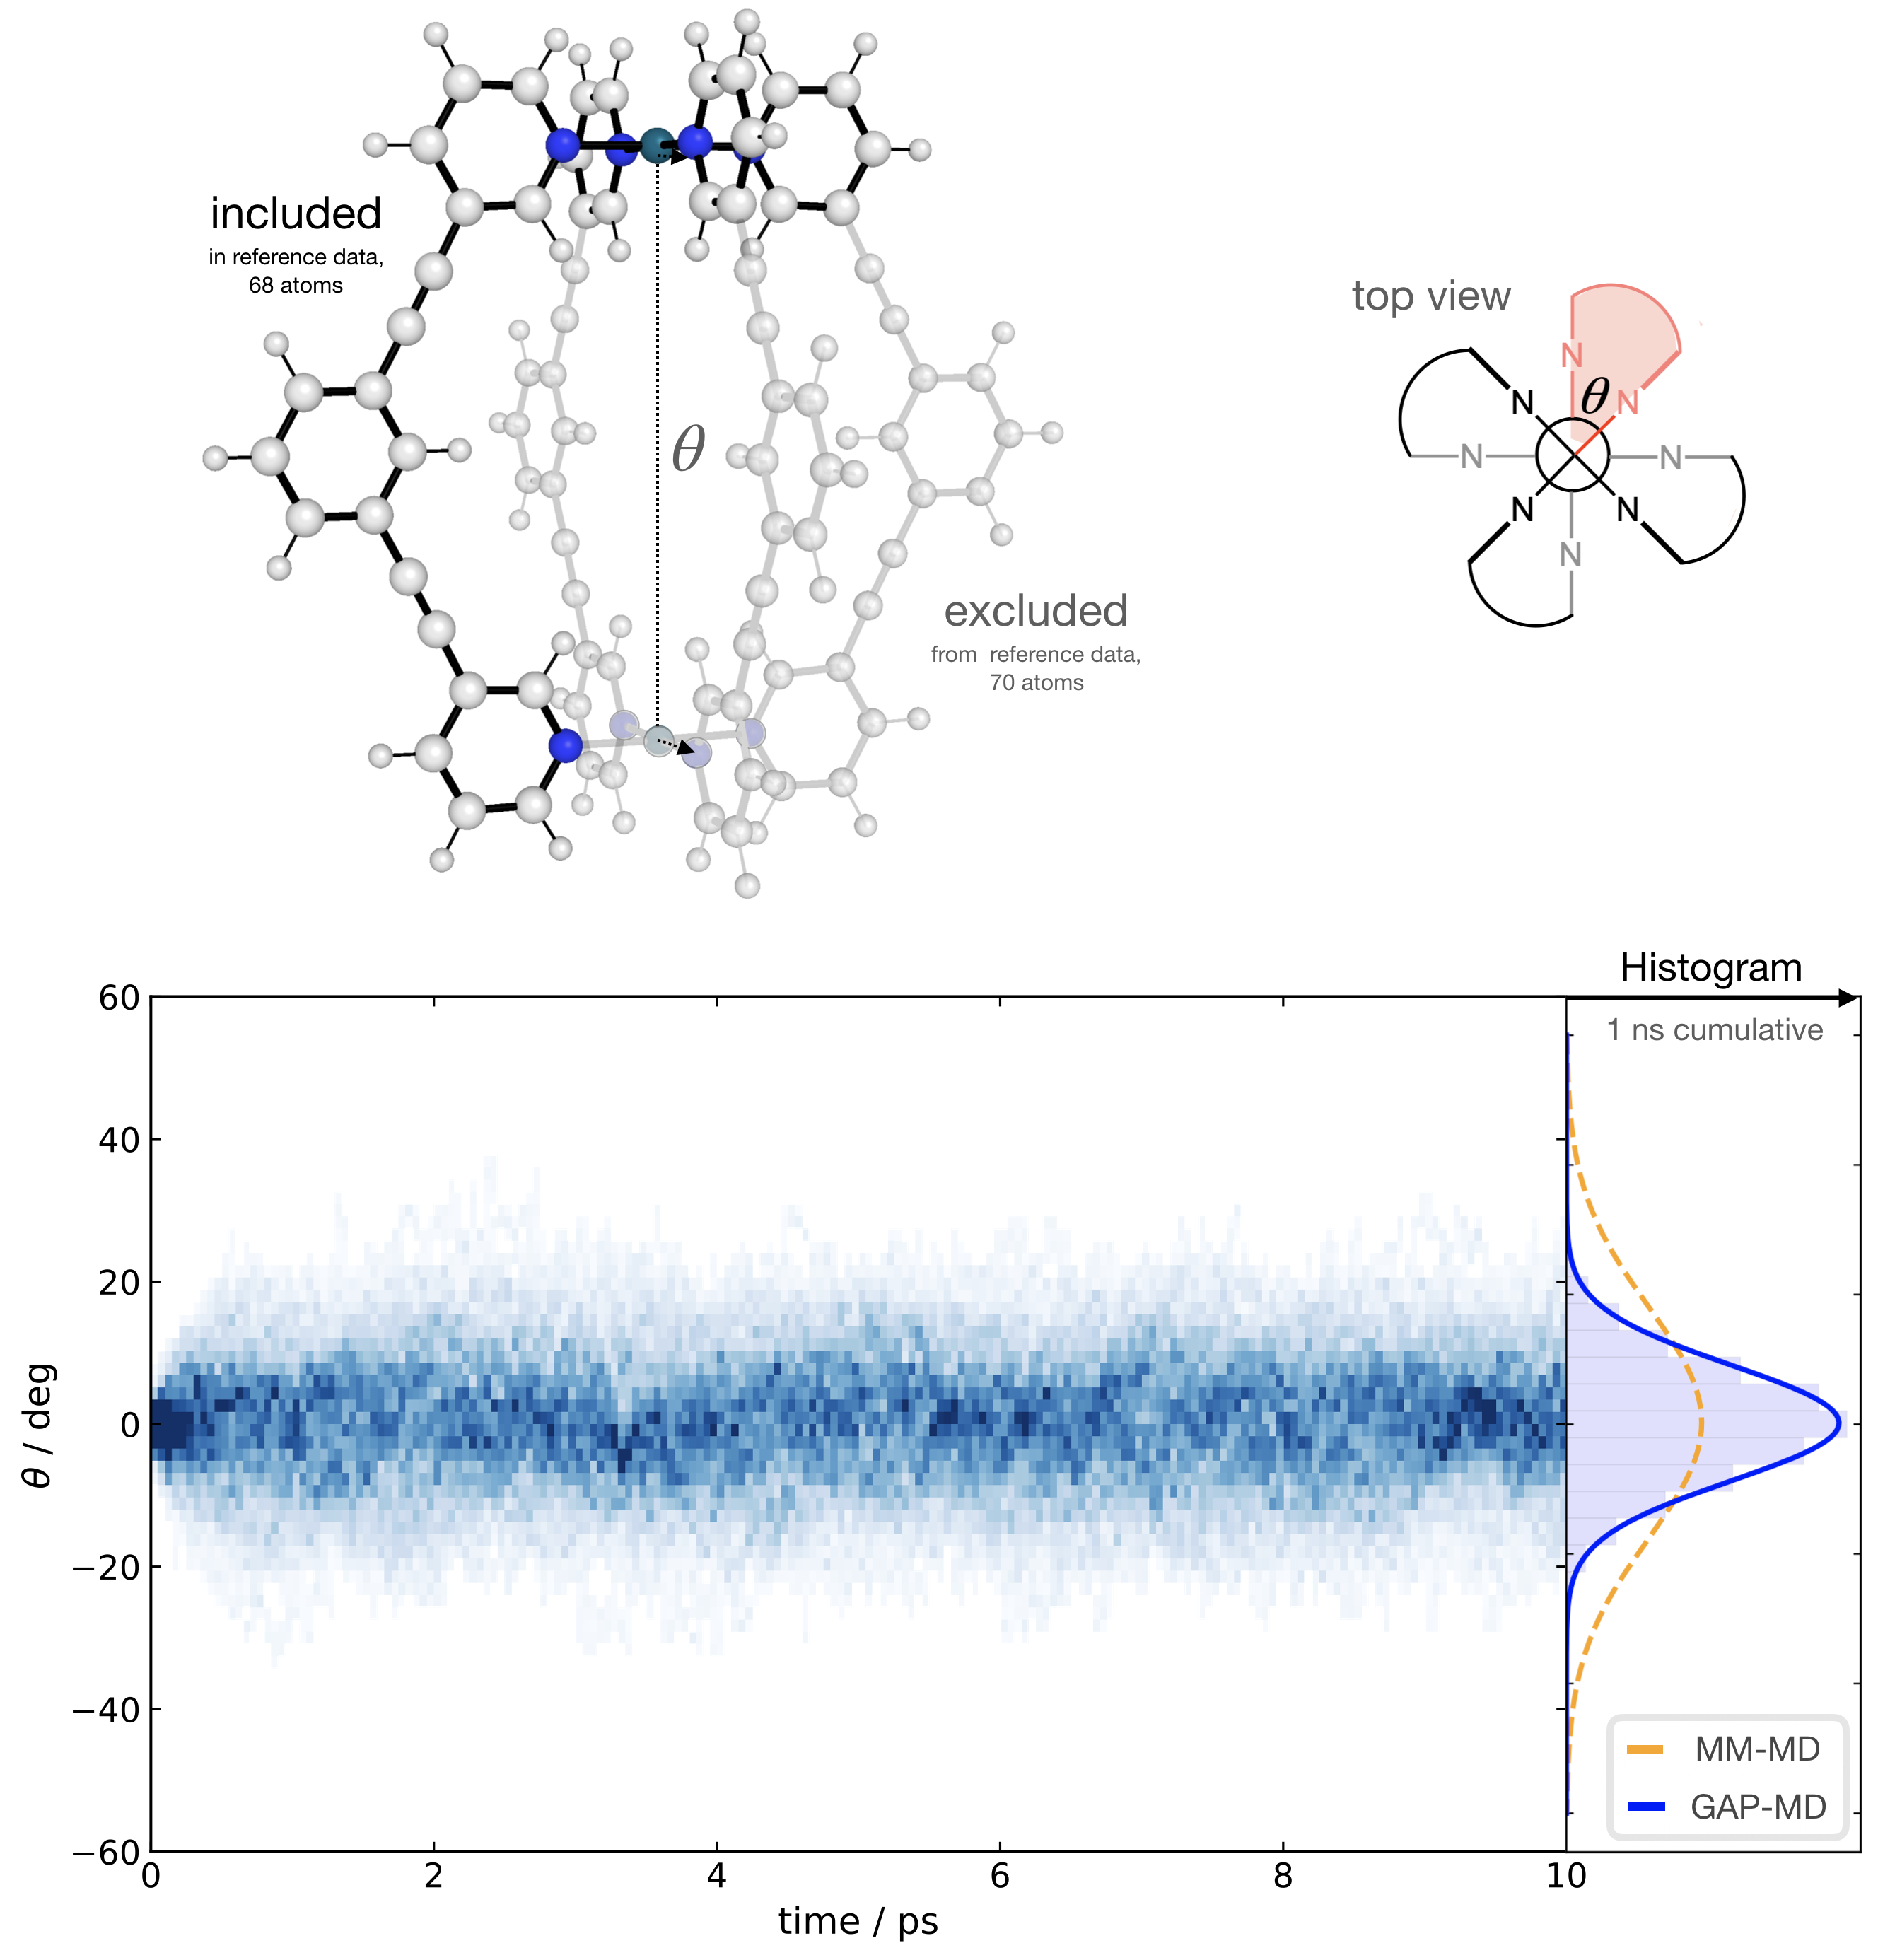
\includegraphics[width=14cm]{6/gap/figs_ms/fig4}
	\vspace{0.2cm}
	\hrule
	\caption{Temporal twist angle $\theta$ for an Temporal twist angle $\theta$ for an [Pd${}_2$L${}_4$]$^{4+}$ metallocage (right) obtained from 100 independent GAP-MD trajectories (each run for 10 ps at 300K), GAP trained on a 68-atom [PdL(py)${}_3$]$^{2+}$ system (py = pyridine), representative of the whole metallocage as shown, at 500 K with a 0.2 eV error threshold for the active-learning protocol. Time-dependent histogram generated from 50 fs time chunks over the whole 10 ps time period. PBE0-D3BJ/def2-SV(P) ground truth surface.}
	\label{fig::ml_4}
\end{figure}


\subsubsection{Reaction Dynamics in Gas and Solvent Phase}

The high dimensionality and ensuing flexibility of ML potentials make them highly suitable to study reaction dynamics – the latter usually require many costly electronic structure calculations to obtain atomic-level descriptions of reaction mechanisms, solvent effects or post-transition state (TS) dynamics.\cite{Pratihar2017, Ess2008} In the following section, we show that our data-efficient strategy enables accurate reactive potentials (\taua $> 100$ fs) with only a few hundreds of DFT evaluations for a set of prototypical organic reactions.

{\bfseries{Gas phase bimolecular nucleophilic substitution}}. The S${}_\text{N}$2 nucleophilic substitution reaction is fundamental in organic chemistry and has been extensively studied using AIMD and analytically fit PES.\cite{Pratihar2017, Xie2016} However, even with efficient approaches to fitting PES, AIMD methods still require tens of thousands of energy evaluations.\cite{Szabo2017} Here, we generated a reactive GAP to study the reaction between chloride and methyl chloride as a prototypical case often employed to validate QM/MM reactions and for which extensive literature exists (see ref. \cite{TiradoRives2019} and references therein). By initialising active learning from the transition state (TS), the true intrinsic reaction coordinate is reproduced to within 1 \kcalx (Figure \ref{fig::ml_si_16}). 


\begin{figure}[h!]
	\vspace{0.4cm}
	\centering
	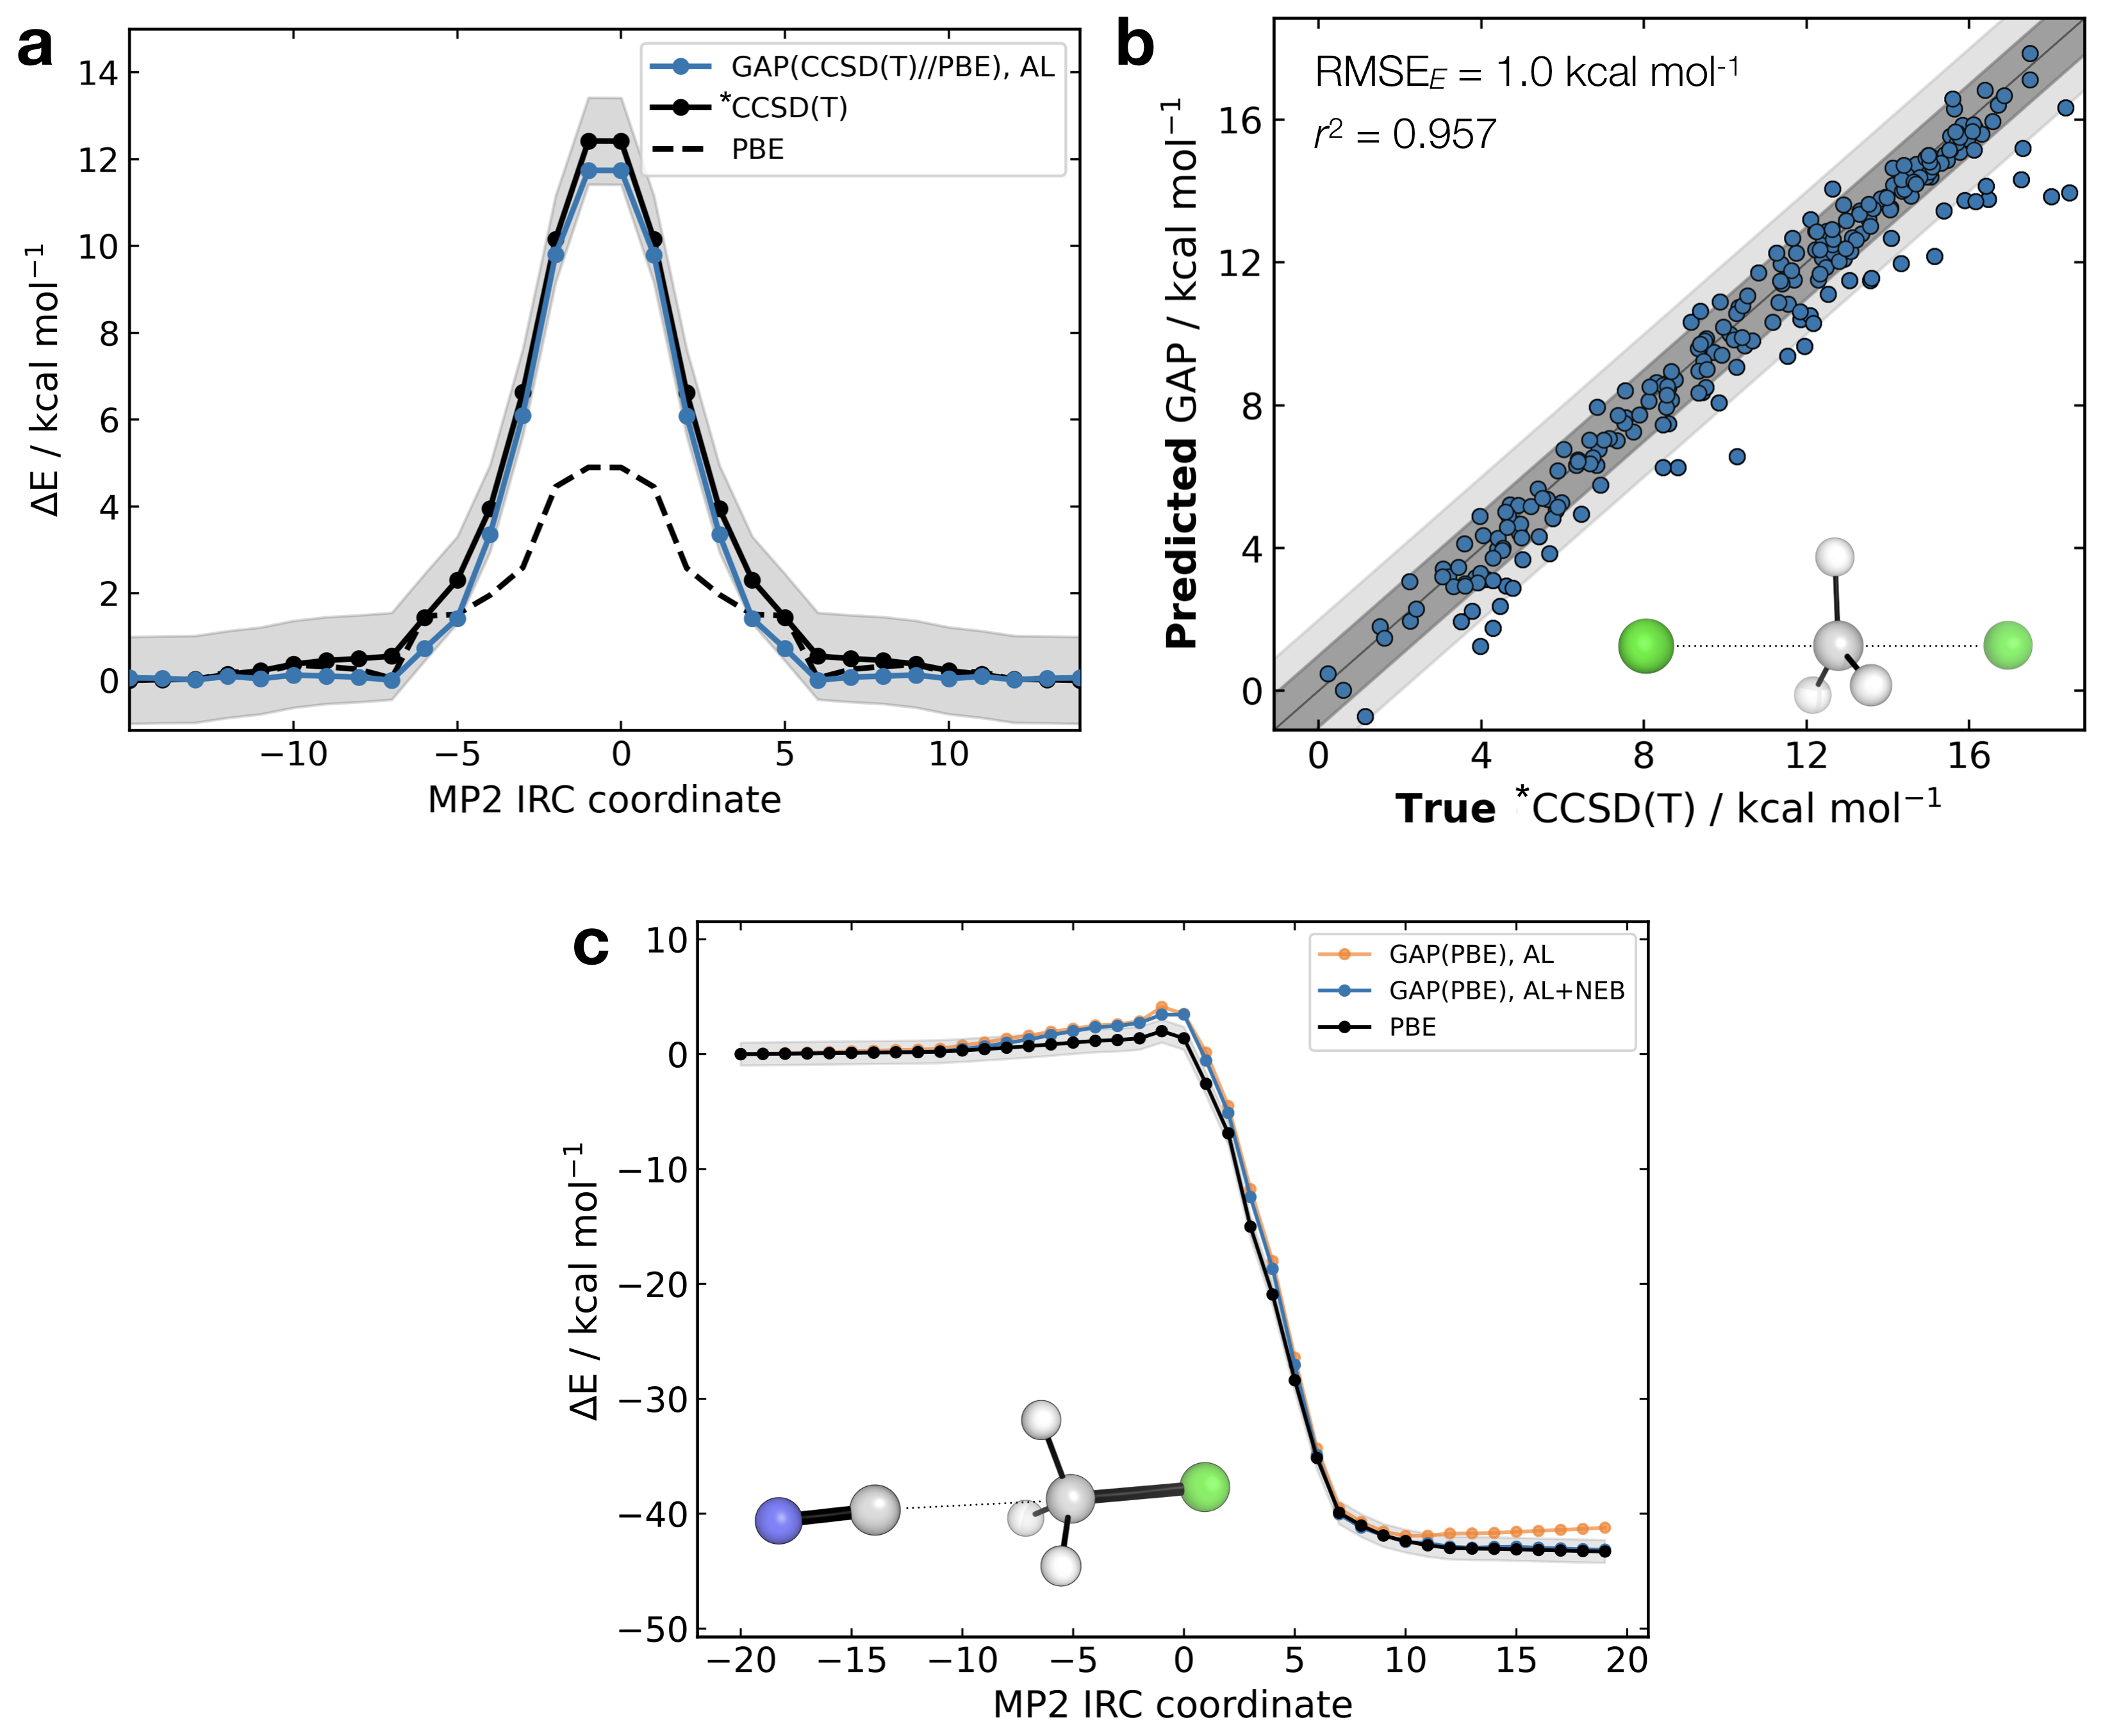
\includegraphics[width=\textwidth]{6/gap/figs_ms/fig5}
	\vspace{0.2cm}
	\hrule
	\caption{Gas-phase S${}_\text{N}$2 reactive dynamics. Energetics of a mode Cl$^{-}$ + CH${}_3$Cl → Cl$^{-}$ + CH${}_3$Cl l S${}_N$2 reaction in the gas phase. (a) Predictions (GAP) and ground-true (*CCSD(T) $\equiv$ DLPNO-CCSD(T)/ma-def2-TZVPP) energy values on the MP2/ma-def2-TZVPP intrinsic reaction coordinate (IRC). Shaded region bounds the ‘chemically accurate’ (±1 kcal mol–1) region. (b) Parity plots of between GAP predictions and true energies from ten 100 fs GAP-MD trajectories initialised from the TS (300 K). Dark and light grey area bound the $\pm$1 \kcalx and $\pm$ 2 \kcalx error regions, respectively. (c) IRC for CN$^{-}$ + CH${}_3$Cl → Cl$^{-}$ + CH${}_3$CN but trained using uphill active learning, with nudged elastic band refinement; see Figure \ref{fig::ml_si_16} for additional details.}
	\label{fig::ml_5}
\end{figure}


Interestingly, and unlike our previous attempt to generate a DFT-quality GAP by evaluating energies and forces on DFTB active-learnt configurations, here, uplifting a DFT-level GAP to an accurate wavefunction-level GAP is possible. This method allows coupled cluster-quality energy profile (Figure \ref{fig::ml_5}a) and dynamics to be propagated from the TS with just 55 energy and (numerical) force evaluations at the CCSD(T) level (Figure \ref{fig::ml_5}b/\ref{fig::ml_si_16}). The resultant GAP is considerably more accurate than the underlying DFT energy profile (dashed, Figure \ref{fig::ml_5}a). Active learning can also be initialised from an association complex and the IRC learned without prior knowledge of the TS. For the exothermic reaction between cyanide and methyl chloride, training from reactants and initialising velocities such that 11 \kcalx (0.5 eV) was present in the breaking bond, the reaction is sampled in the training (Figure \ref{fig::ml_si_16}c). Relaxing a nudged elastic band (NEB) using the trained GAP over an interpolated path between reactants and products affords an IRC within chemical accuracy of the true profile (RMSE= 0.9 \kcal, Figure \ref{fig::ml_5}c). In this case, adding a NEB refinement step to the training is essential to adequately sample the product region and reach chemical accuracy in the reaction energy (orange vs. blue lines Figure \ref{fig::ml_5}c). Here, uplifting the GAP to CCSD(T) affords chemical accuracy in the minima and TS regions, with a more limited accuracy in the region in between (Figure \ref{fig::ml_si_16}d); this is likely due to the large differences between the PBE and CCSD(T) surface in that region. Despite this, the uplifted profile is considerably more accurate than the underlying DFT (Figure \ref{fig::ml_si_16}d).


{\bfseries{Post-TS bifurcating pathway in a Diels-Alder reaction}}.  GAPs for more complex reactions involving reactions that proceed on a bifurcating PES can also be trained. These reactions typically require AIMD simulations, where selectivity is determined from the average behaviour of many trajectories leading to either product. Other approaches have also been developed.\cite{Lee2020} We explored the dimerisation between cyclopentadiene, for which endo selectivity has been rationalised on the basis of bifurcating reaction pathways.\cite{Caramella2002} Once again, initiating active learning from the literature TS (TS${}_1$, Figure \ref{fig::ml_6}) and using a DFT method analogous to the one used in the original work by Caramella and co-workers we obtain a reactive potential from which 500 fs trajectories were propagated. Interestingly, we found that propagating the system from this TS did not afford any products (P${}_1$ or P${}_2$, Figure \ref{fig::ml_6}), with all trajectories leading to the reactant state (Figure \ref{fig::ml_si_18}).


\begin{figure}[h!]
	\vspace{0.4cm}
	\centering
	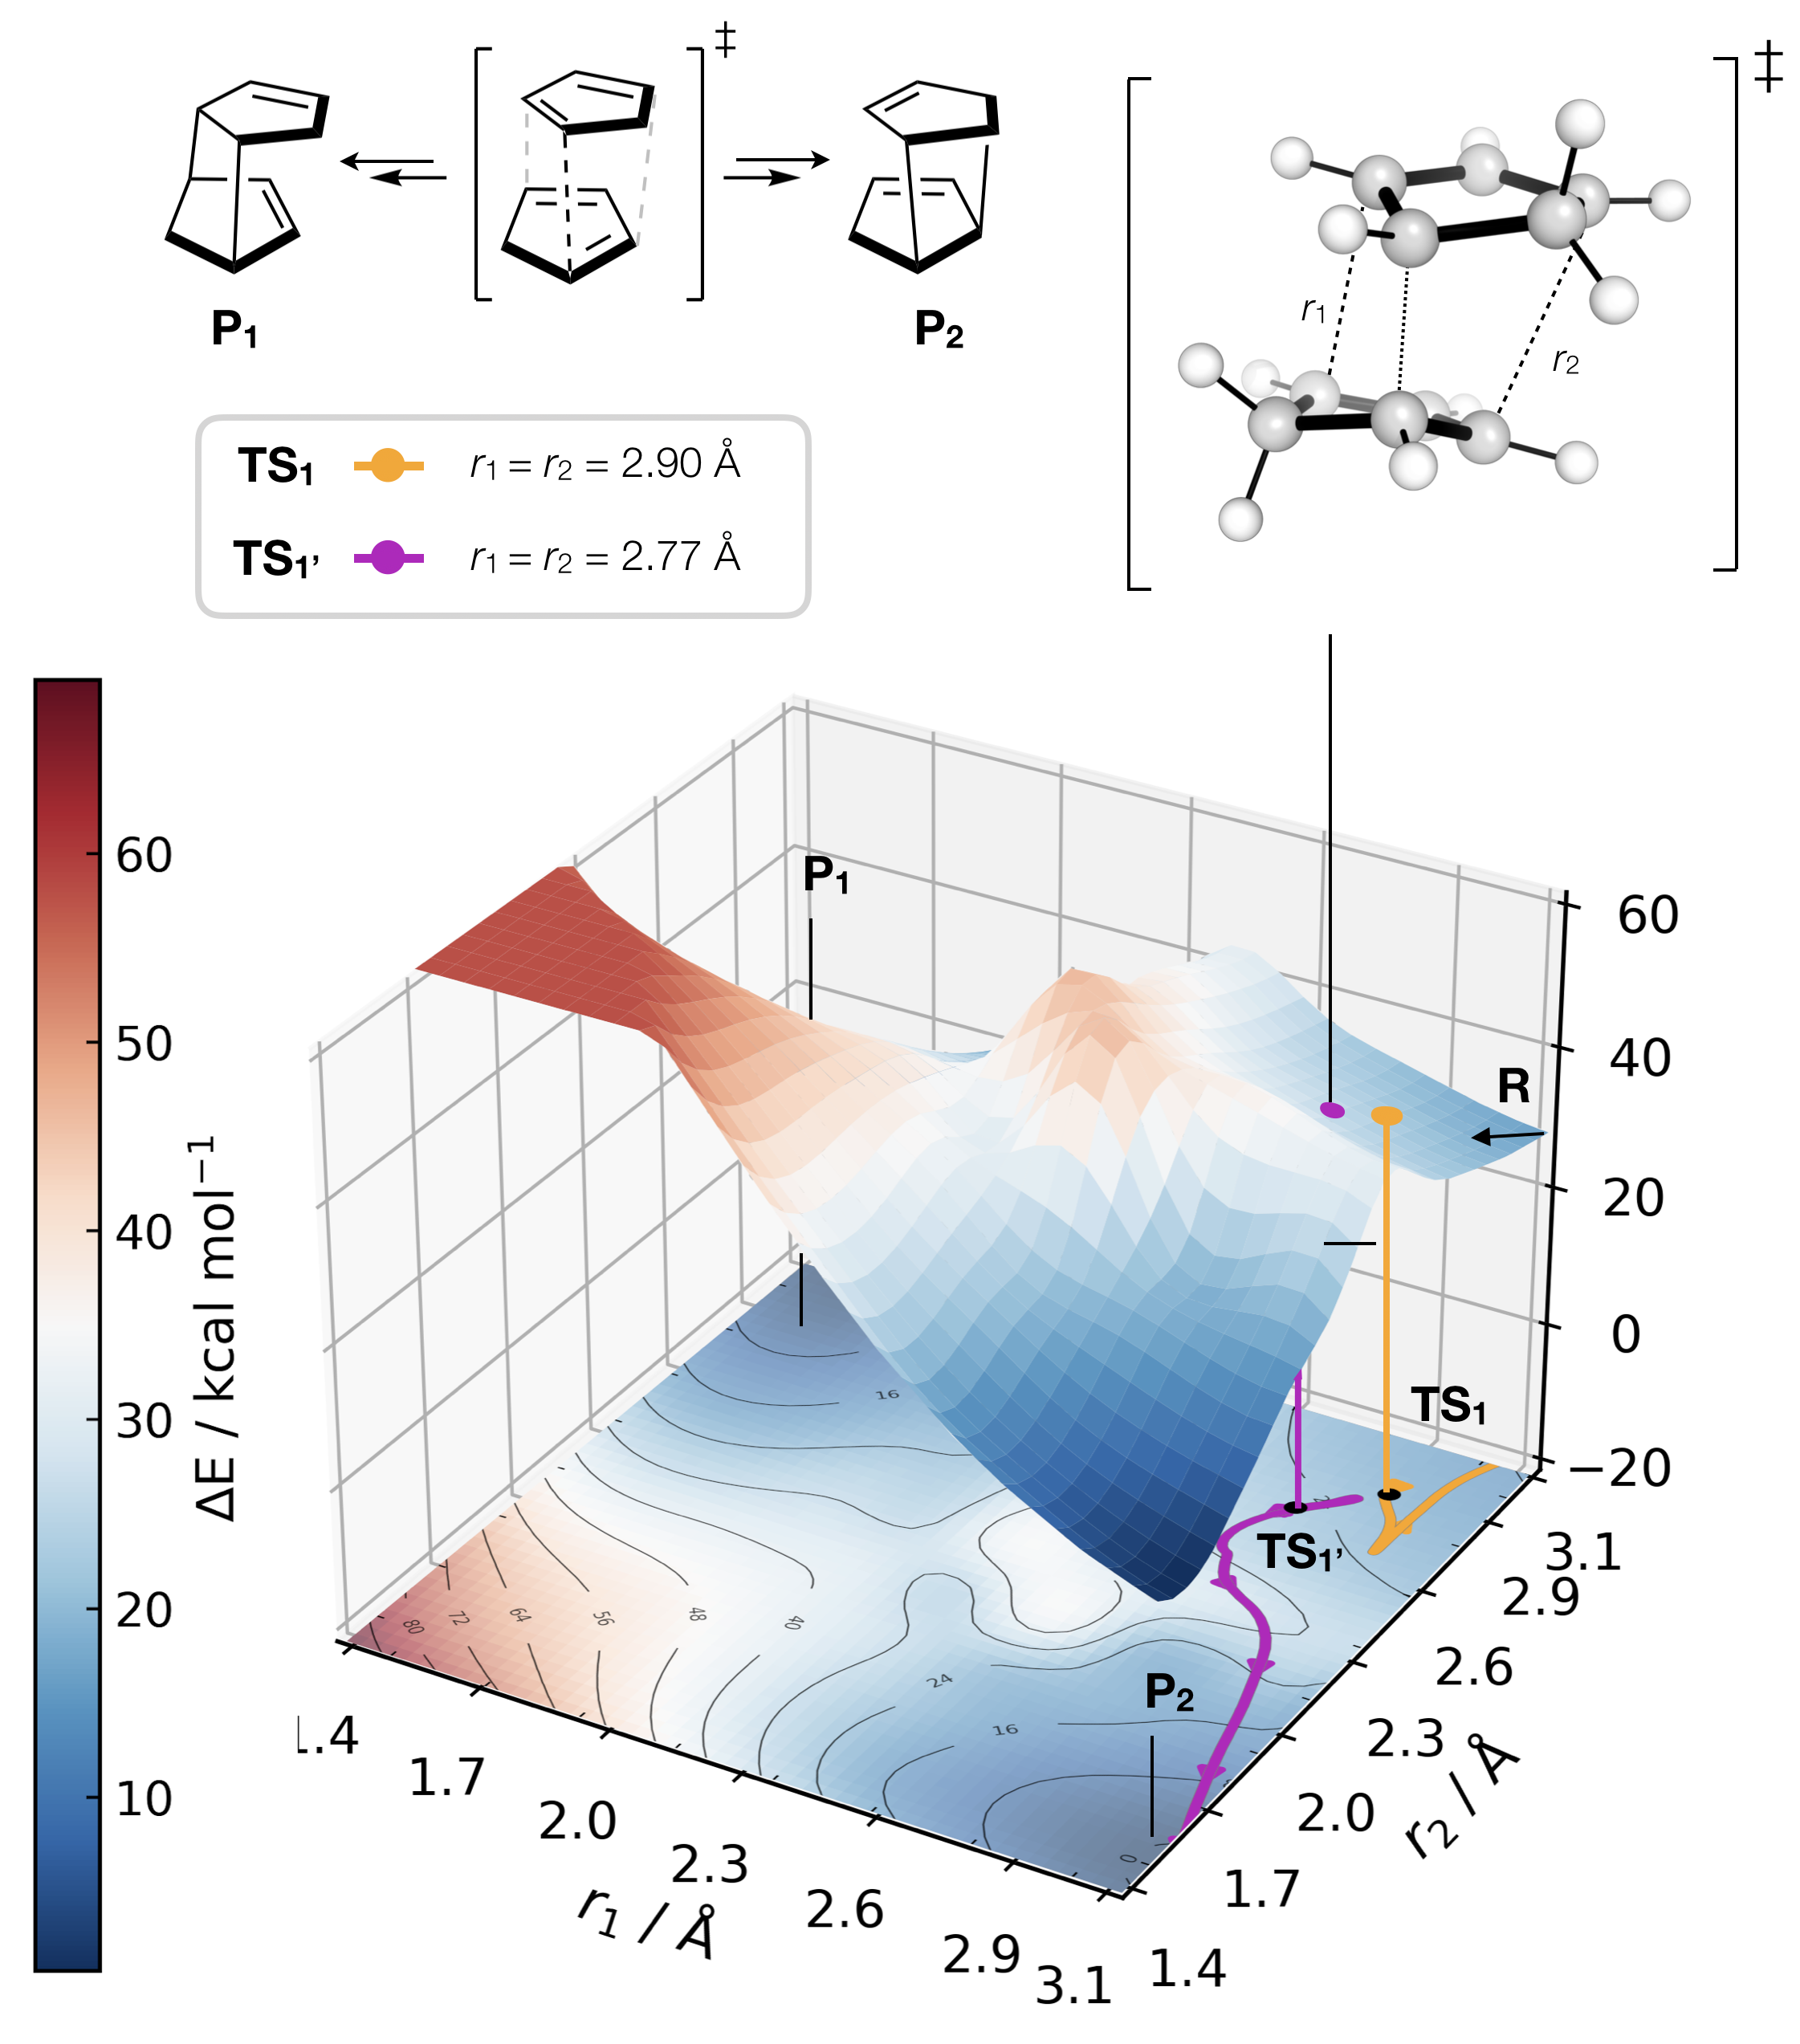
\includegraphics[width=10cm]{6/gap/figs_ms/fig6}
	\vspace{0.2cm}
	\hrule
	\caption{GAP dynamics on a bifurcating surface. 2D PES (B3LYP/def2-SVP) along the forming bond distances ($r_1, r_2$) in the dimerisation of cyclopentadiene. An example of GAP-propagated reactive dynamics (300 K) is shown from TS${}_1$ ($7_N$ in ref. \cite{Caramella2002}), which leads to reactants, (representative trajectory in orange), and from TS${}_1’$ which leads to products (a representative trajectory is shown in purple). 3D projection is truncated at 2.5 eV above the minimum for plotting. Interpolated surface used a cubic spline using \emph{scipy.interp2d} with the raw surfaces shown in Figure \ref{fig::ml_si_21}. All trajectories shown in Figure \ref{fig::ml_si_18} and \ref{fig::ml_si_20}.}
	\label{fig::ml_6}
\end{figure}

Further investigation and generation of the relaxed 2D potential energy surface over the two possible forming C–C bonds ($r_1, r_2$) leading to products provided a rather different surface to the one suggested in ref. \cite{Caramella2002}, with a flat portion then an incline as $r_1, r_2$ shorten below 2.9 \AA, with a steeply exergonic reverse reaction (intrinsic reaction coordinate, IRC, see full Supporting Information). As noted by Caramella, following the IRC forwards from TS1 the reaction proceeds to another TS1’ which is similar in energy ($\Delta E = 2$ \kcal). By training a GAP at 500 K and propagating GAP-MD from TS1’ and sampling the area of the PES around a valley-ridge inflection point (VRI), trajectories lead to the expected two products (e.g., purple line, Figure \ref{fig::ml_6} and Figure \ref{fig::ml_si_20}). This example demonstrates that with no a priori knowledge, apart from the structure of TS${}_1$, the topology of the bifurcating surface can be revealed efficiently using GAP dynamics. This strategy is completely automated, requiring training of a few hours to days, thus providing a promising approach to routinely examine reaction dynamics in organic molecules.


{\bfseries{Solution phase bimolecular nucleophilic substitution.}} The ability to accurately describe bond-breaking/forming paths in the condensed-phase is crucial if this strategy is to be applied to increasingly complex processes, such as enzymatic reactions. Towards this goal, and having generated potentials for condensed-phase molecular systems and gas-phase reactions, we decided to extend our active learning strategy to explicitly solvated reactions; once again, using the S${}_\text{N}$2 reaction between chloride and methyl chloride as a test case. S${}_\text{N}$2 reactions have been used as a test case for a recent ML potential, but those studies have been limited to the gas phase and used thousands of training points.\cite{Unke2019} Literature examples of ML potentials to study reactions in explicit solvent are limited. Recently, Parrinello and co-workers reported an NN potential to study urea decomposition in water.\cite{Yang2021} Training a model for the implicitly solvated reaction proceeds in a similar way as for the gas phase analogue and affords a surface close to the ground truth (Figure \ref{fig::ml_7}a).



\begin{figure}[h!]
	\vspace{0.4cm}
	\centering
	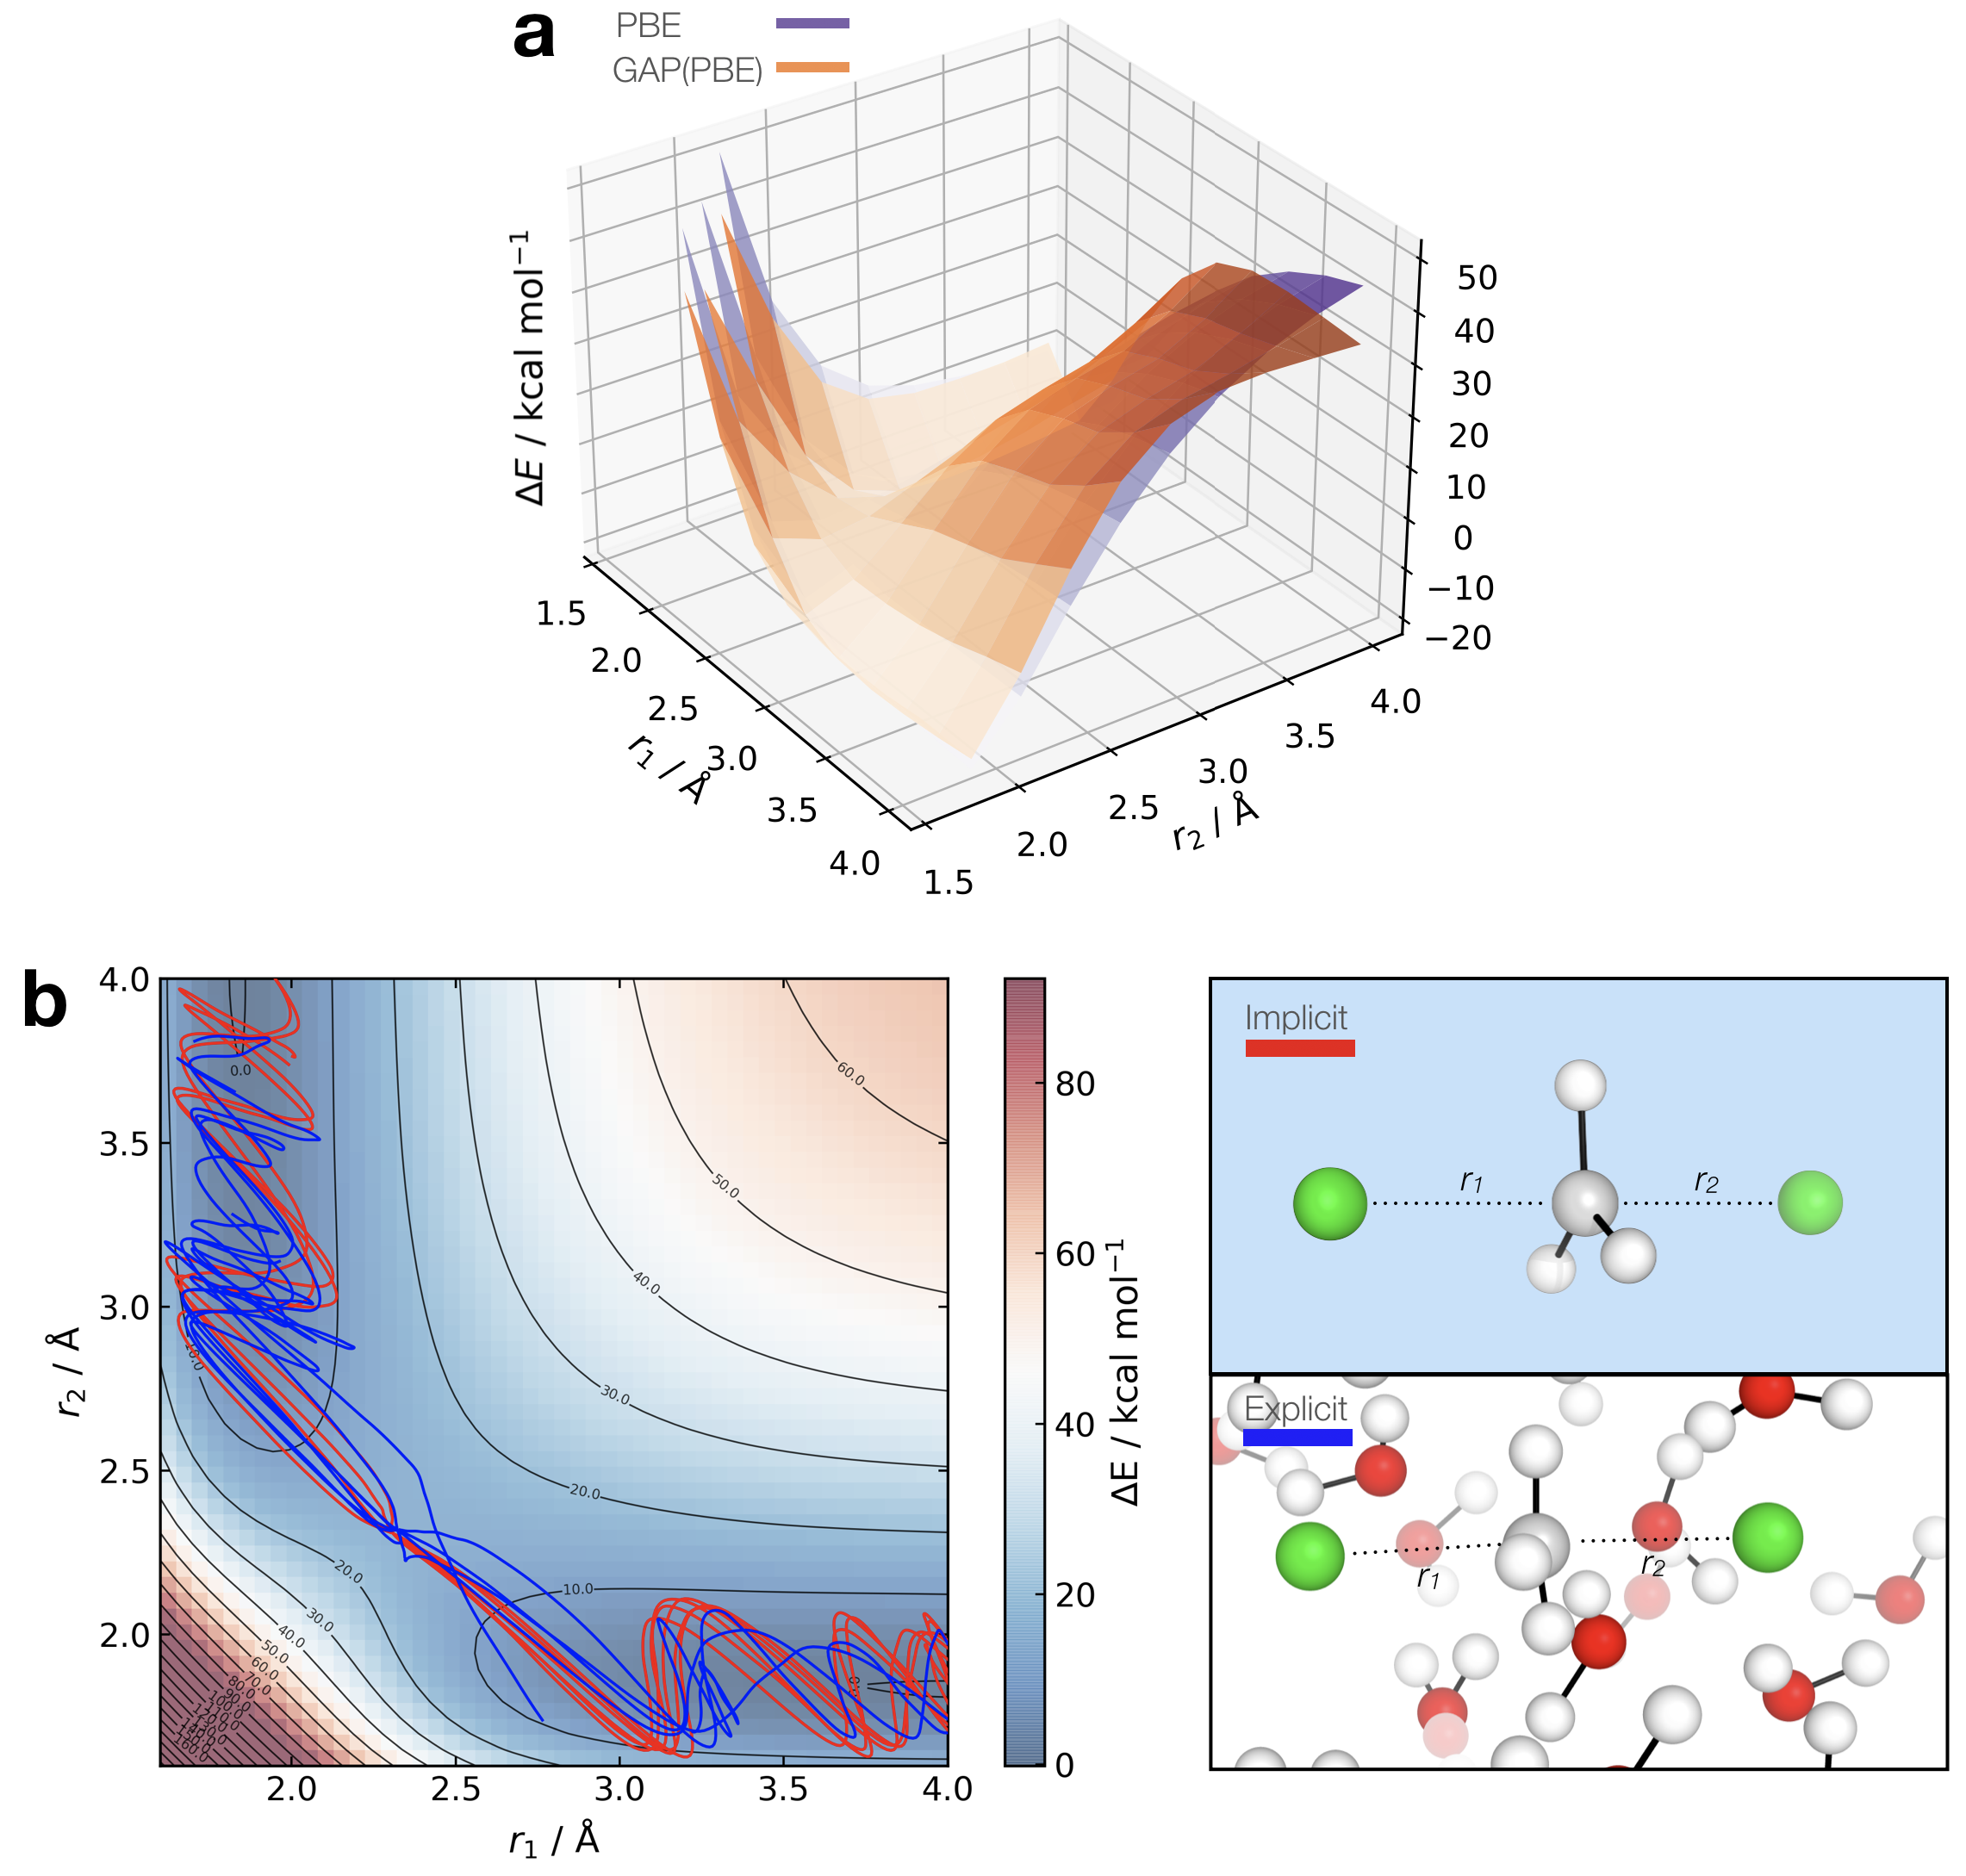
\includegraphics[width=14cm]{6/gap/figs_ms/fig7}
	\vspace{0.2cm}
	\hrule
	\caption{Solution-phase S${}_\text{N}$2 reactive dynamics. (a) True (CPCM(Water)-PBE/def2-SVP, purple) and GAP predicted relaxed 2D PESs in implicit solvent, zeroed to the transition state energy. (b) Reactive GAP MD trajectories (lines) propagated from the TS, trained on implicitly solvated configurations (CPCM(Water)-PBE/def2-SVP, red) and explicitly solvated configurations (PBE/400 eV, blue). Ground truth implicitly solvated surface (cubic interpolated, 5:1) underneath with the error to the GAP prediction in Figure \ref{fig::ml_si_23}. Intramolecular GAP used C-only ($r_c^\text{SOAP}$ = 6 \AA) descriptor with the intermolecular explicit solvent using a SOAP on O ($r_c^\text{SOAP}$ = 3.5 \AA) and Cl ($r_c^\text{SOAP}$ = 4.5 \AA, Figure \ref{fig::ml_si_24}).}
	\label{fig::ml_7}
\end{figure}



Adopting an identical strategy to the one employed for condensed phase systems, the intra- and inter-molecular PES dynamics can be propagated from the TS and the effect of explicit solvation interrogated (Figure \ref{fig::ml_7}b). This only requires knowing a priori the gas-phase TS for the training to be complete in explicit water. Interestingly, the behaviour in explicit water (blue, Figure \ref{fig::ml_7}b) differs from the implicit counterpart (red, Figure \ref{fig::ml_7}b). This can be understood considering that in implicit solvent reorganisation is instantaneous, which results in oscillations in the C-Cl bond characteristic of a gas phase reaction. In contrast, the dynamics are more complex in explicit solvent, with a slower transition from the product channel. Additionally, one of the 10 trajectories re-crosses the barrier after 170 fs of simulation (Figure \ref{fig::ml_si_22}), where the solvent has not reorganised to accommodate the anionic chloride yet, making the path to products shallower in energy.

The component-wise separation of the system also leads to the possibility of training to a more accurate ab initio surface for the gas phase reaction, in a similar way to QM/MM, but here a ML(A)/ML(B) partition is available where A and B are two different ground truth methods. Application of this kind of hierarchical ML potential fitting will be the subject of further work.


{\bfseries{Limitations.}} In its current implementation, this method is well suited for studying systems of up to 50 atoms if training is expected to be completed in a day, using a single node of 20 CPUs. For larger systems, the speed will depend on the complexity of the PES, where even using inexpensive methods thousands of training configurations and several iterations cycles may be needed to learn the different atomic environments. In contrast, training can be achieved efficiently for large systems with higher symmetry, and effectively lower dimensional PES. This is the case, for example, for the supramolecular cage shown above, which contains 138 atoms and can be modelled in full with GAP only using 68 atoms for training (Figure \ref{fig::ml_4}). Furthermore, the current intra+intermolecular decomposition remains fixed throughout the simulation making the water potential generated initially incapable of auto-ionisation. Re-determining the connectivity (and therefore re-assigning the “intra” components) every few steps during the simulation might help to address this limitation. However, provided the model has been trained in a region where a chemical change has occurred, the molecular components in that region do not need to retain their connectivity. This is the case, for example, in the S${}_\text{N}$2 reaction shown in Figure \ref{fig::ml_7}, where connectivity changes between the two molecular units that constitute the solute.


\subsection{Conclusion}

Studying dynamic processes and the effect of explicit solvation on chemical reactions demands a rapid method to develop bespoke force-field models with high accuracy. Here, we demonstrated that within the Gaussian Approximation Potential (GAP) machine learning framework, accurate and robust models can be developed efficiently for gas-phase and condensed-phase molecular reactions. Our strategy starts from a small number of randomly selected points in the configuration space, from which active learning training of intra- and inter-molecular components of the energy and forces is carried out. The developed method is publicly available ({\color{blue}{https://github.com/duartegroup/gap-train}}). We also define a prospective error metric, which is found to be crucial in developing robust active-learning-based potentials, whereas correlation on a predefined test set is insufficient to assess the quality of such a potential. We illustrate the generality of this approach by modelling bulk water, Zn(II) in aqueous solution, and chemical reactions in the gas phase and explicit solvent, including post-TS cyclisation and S${}_\text{N}$2 reactions. The diversity of the examples presented here demonstrates the general applicability of the strategy and encourages applying this approach in the modelling of more complex reactions in homogeneous and heterogeneous environments.



\subsection{Methods}

All Gaussian Approximation Potentials (GAPs) were trained using the GAP and QUIP codes (Singularity distribution, commit \# 66c553f) and a Smooth Overlap of Atomic Positions (SOAP)\cite{Bartok2013} kernel with hyperparameters as defined in Table S1. For a single component condensed phase system such as water, two GAPs are fitted for the intra and intermolecular components, respectively, while for the solute-solvent systems, such as the S${}_\text{N}$2 reaction between chloride and methyl chloride, three GAPs were fitted: one for the gas-phase solute, a second for gas-phase solvent and a third one for the intermolecular interactions; see Table S2, entry 6 for details. An example of the input script required to train a bulk water model is shown in Figure \ref{fig::ml_8}. In all systems the intramolecular water potential was trained at the reference level on an evenly spaced grid (512 points, $r_\text{OH}$ = [0.8–1.5] \AA, $r_\text{HH}$ = [1.0–2.5] \AA). Other intramolecular GAPs employed SOAP descriptors with cut-offs shown outlined in the figure captions. Intermolecular GAPs were trained by subtracting intramolecular energies and forces of all the defined components from the reference total energy. All pure condensed phase systems were trained and simulated at or close to their experimental liquid densities using 10 solvent molecules (e.g. 10 H${}_2$O in a 343 \AA${}^3$ cubic box). Aqueous Zn and explicitly solvated S${}_\text{N}$2 reactions used 20 water molecules in a cubic box with side length of 10 \AA. All files required to reproduced the examples shown here can be found in {\color{blue}{https://github.com/duartegroup/gap-train/tree/master/examples/paper\_examples}}.

GAP-MD simulations were performed with ASE\cite{HjorthLarsen2017} interfaced to QUIP with the quippy wrapper using the Langevin integrator with 0.5 fs timesteps at 300 K unless otherwise specified. Condensed phase MD simulations were performed with three-dimensional periodic boundary conditions following minimisation and equilibration for at least 20 ps. Initial configurations, CUR\cite{Mahoney2009} selection and all learning curves were generated with the \emph{gap-train} module, which was used to run the automated fitting.\cite{gaptrain} All active learning was performed using a ‘diff’ strategy, where a configuration is added to the training set if $|E^0 – E^\text{GAP}|$ is larger than a threshold. With system-dependent hyperparameter optimisation, using a threshold on the maximum atomic variance predicted by the Gaussian process (‘gp\_var’) can result in accelerated learning (Figure \ref{fig::ml_si_21}). CUR selection used SOAPs averaged over atoms in a configuration using the Dscribe\cite{Himanen2020} package (`inner’ averaging, over entries of the expansion coefficient vector). Intra+Inter (I+I) energy and force evaluations used an expansion factor of 10 to ensure no intermolecular atoms were within the intra GAP cut-off. The NumPy\cite{Numpy} implementation introduces a negligible computational overhead for expanding the box (~0.1 ms step-1 real time) but requires two GAP calculations on the inter and intra components, currently carried out in serial. All generated potentials, with the exception of the revPBE0-D3 water potential and metallocage, were trained in less than a day on 10 CPU cores. The revPBE0-D3 water potential was constructed without any prior data in 5 days (1 intra + 4 inter) and used 20 CPU cores, while the metallocage fragment was trained for 3 days also on 20 CPU cores. Explicit S${}_\text{N}$2 reaction dynamics was performed using intra components for H${}_2$O and [Cl$\cdots$CH${}_3$Cl]${}^{-}$, where the latter, due to the finite atomic cut-off employed, has the correct dissociation behaviour when Cl${}^{-}$ and CH${}_3$Cl are distant.

Periodic DFTB calculations performed with DFTB+\cite{Hourahine2020} using 3ob\cite{Gaus2013} parameters, and molecular equivalents using GFN2-XTB\cite{Bannwarth2019} in XTB v. 6.2.3. Periodic pure DFT calculations were performed with GPAW\cite{Mortensen2005, Enkovaara2010} v. 19.8.1 with the PBE\cite{Perdew1996} functional and a 400 eV plane-wave cut-off from a dzp LCAO initial guess at the gamma point. Hybrid periodic DFT calculations with the revPBE0\cite{Zhang1998, Adamo1999} functional combined with the D3\cite{Grimme2010} dispersion correction were performed with CP2K.\cite{Kuhne2020}

Molecular DFT, MP2 and coupled cluster [DLPNO-CCSD(T)] calculations performed with ORCA\cite{Neese2012, Neese2017} v. 4.2.1 wrapped with \emph{autodE}\cite{autodE} using PBE\cite{Perdew1996} and PBE0\cite{Adamo1999} functionals, (ma)-def2-SVP, def2-TZVP, ma-def2-TZVPP basis sets\cite{Weigend2005} AIMD calculations at the DFTB level performed with DFTB+ with 3ob parameters\cite{Gaus2013} and MM simulations performed with GROMACS\cite{Berendsen1995, Abraham2015} 2019.2 with TIP3P parameters.\cite{Jorgensen1983} 
\
Behler NN\cite{Behler2007} trained on 7258 RPBE configurations from ref. \cite{Morawietz2016}, re-evaluated at DFTB(3ob) with n2p2\cite{Singraber2019} using the default parameters and symmetry functions. 


\begin{figure}[h!]
	\vspace{0.4cm}
	\centering
	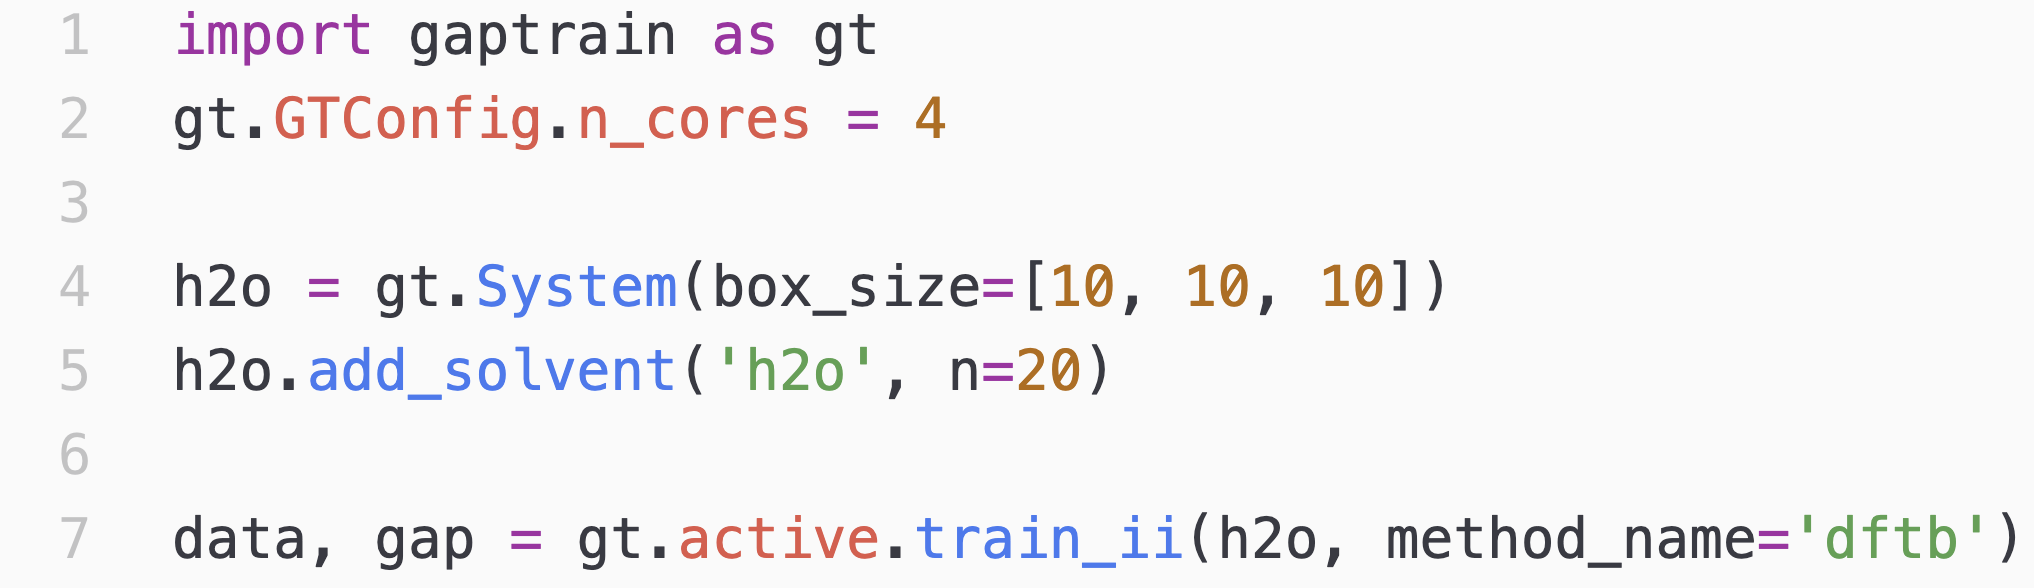
\includegraphics[width=11cm]{6/gap/figs_ms/fig8}
	\vspace{0.2cm}
	\hrule
	\caption{Example Python input script required to train a bulk water model from scratch at the DFTB level using four CPU cores.}
	\label{fig::ml_8}
\end{figure}



\clearpage
\section{Selected Supporting Information IV}
\emph{Full Supporting Information can be found at}: {\url{https://doi.org/10.26434/chemrxiv.13856123}}


\begin{figure}[h!]
	\vspace{0.4cm}
	\centering
	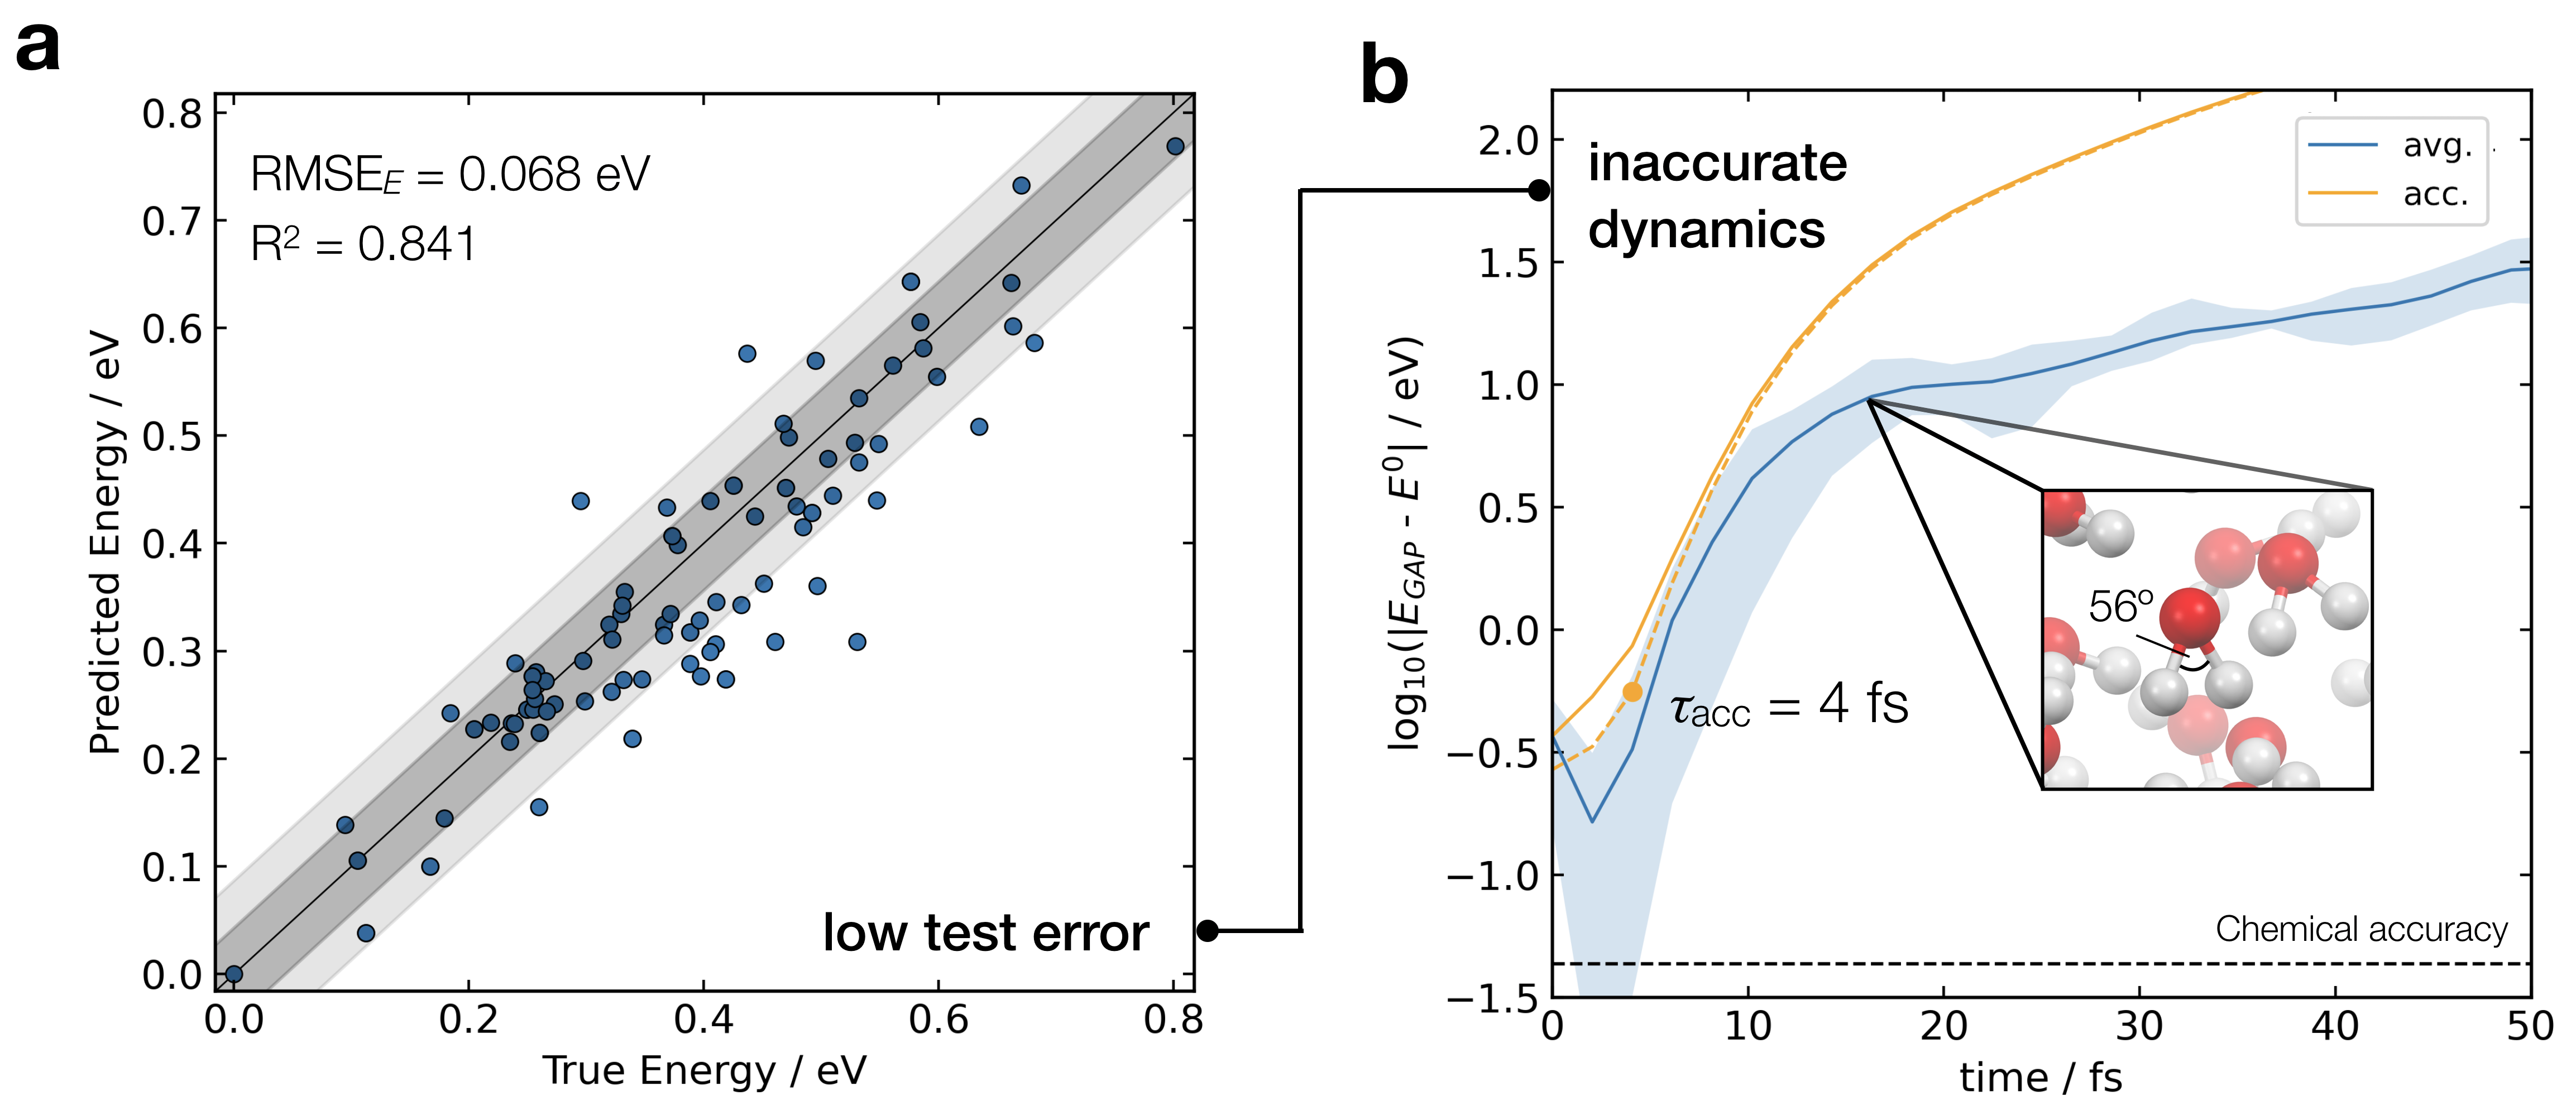
\includegraphics[width=\textwidth]{6/gap/figs_si/fig1}
	\vspace{0.2cm}
	\hrule
	\caption{(a) A GAP model for molecular water (fitted using the P1 parameter set, Table S1) as characterized by its
accuracy on external validation data not encountered in training; dark and light shaded area bound the ‘chemically accurate’ $\pm1$ \kcalx and $\pm2$ \kcalx regions, respectively. (b) the resulting difference between predicted and true single point energies on MD frames at 300 K ($\delta t$ = 0.5 fs). Dynamics with 30 water molecules in a cubic box (l = 10 \AA, $\rho \sim 1$ g cm${}^{-3}$). Error range (min–max, shaded) and average of five simulations using the same trained GAP from different initial randomly placed then minimized points. DFTB(3ob) ground truth. Orange lines depict the total cumulative error (solid) and cumulative error above 0.1 eV (dashed).}
	\label{fig::ml_si_1}
\end{figure}





\begin{table}[h!]
	\def\arraystretch{1.5}
	\begin{tabularx}{\textwidth}{YYYY}
		\hline
		Set	   &Type&	Parameter	&Value\\
		\hline
		
		&        	&$\sigma_E$	&0.316 meV
\\
	   &GAP   & $\sigma_F$	&0.1 eV \AA${}^{-1}$
\\
	    &           & $\zeta$    &  	4
\\
	    &	       &   $r_c$	&  5.5 \AA \\
	   &                 & $n_\text{sparse}$&	30
\\
	    &2b descriptors: & $\delta_{2b}$ &	1.0 eV
\\
      	& O--H, H--H, O--O   &$\theta$	    & 1.0 \AA  \\
	P1 &                        &sparse method	& Uniform
\\

         &							& $r_c$&3.0\AA\\
        &						& $n_\text{sparse}$ &100\\
		&						&  $\delta_\text{SOAP}$&0.1eV\\
		&SOAP descriptor: O&$\sigma_\text{at}^\text{SOAP}$&0.5\AA\\
		&&$n_\text{max}, l_\text{max}$& 6 \\
	    &                      &  sparse method	    & CUR points
 \\
	 \hline
	    &	 GAP	   &  $\sigma_E$	&        0.316 meV  \\
        &	               &   $\sigma_F$	&  	0.1 eV \AA${}^{-1}$
 \\
	     &                  & $\zeta$         & 	4
  \\
	    &                   &	$r_c$	             & various
\\
     	&                  & $n_\text{sparse}$	       &500
\\
	P2 &SOAP descriptors  &$\sigma_\text{at}^\text{SOAP}$	&0.5 \AA
\\
	    &                   &$n_\text{max}, l_\text{max}$&6
\\
	   &                    &sparse method	&CUR points
	\end{tabularx}
	\hrule
	\caption{Parameter sets for GAPs, SOAPs and 2/3b descriptors.}
	\label{table::ml_si_1}
\end{table}





\begin{table}[h!]
	\def\arraystretch{1.5}
	\begin{tabularx}{\textwidth}{sbss}
		\hline
		Strategy  &	Notes&	\taua / ps&	$N$\\
		\hline
		MM-MD & 
		{\small{Classical molecular mechanics MD simulations were performed at 100, 300, 500 and 1000 K using GROMACS v. 2019.2 with a timestep of 1 fs and TIP3P water. Following a 1 ns NVT equilibration of a random configuration of water 10 ns of NVT dynamics were performed taking 1000 evenly spaced frames from the simulation. }}
		& 0 & 	1000 \\
		
		rand. &
		{\small{Configurations are /were generated by adding GFN2–XTB optimised water molecules into the box in a random position and orientation, ensuring that there are no intermolecular distances < 1.5 \AA. Random displacements are/were added to each Cartesian coordinate sampled from a random normal distribution with $\sigma=0.05$ \AA, which samples over intramolecular bond stretches and bends.
		}} & 0 & 1000 \\
		
	   rand. min. &
		{\small{As rand. where each random configuration is minimized to $|F_i| < 1$ eV \AA${}^{-1}$, where $F_i$ is the force on atom $i$. Subsequently, random normal displacements were added to each atom to ensure some sampling of the intramolecular modes.
		}} &   0.0008 $\pm$ 0.0007	& 7490 $\pm$20 \\
	
		AIMD&
		{\small{Ab-initio MD simulations were performed at the ground truth level (DFTB, 3ob parameters) for 1 ps at 300 K with a 0.5 fs timestep. Frames are randomly selected from the trajectory with at least a 2 fs interval.
		}} &   0.011 $\pm$ 0.003 & 2570 $\pm$  10 \\
	
	\end{tabularx}
	\hrule
	\caption{Outline of training strategies used to train a GAP for bulk water (Figure \ref{fig::ml_1}). $N$ total ground truth evaluations used to train the final potential. Errors are quoted as standard errors in the mean from 5 independent samples where appropriate to one significant figure. All training used 10 water molecules in a cubic box with side length 7 \AA.}
	\label{table::ml_si_2}
\end{table}
	
	
\begin{table}[h!]
	\def\arraystretch{1.5}
	\begin{tabularx}{\textwidth}{sbss}
		\hline
		Strategy  &	Notes&	\taua / ps&	$N$\\
		\hline
		 AL&
		{\small{Active learning is initiated from a GAP trained on 10 random configurations with a 1.5 \AA$\;$ minimum distance between water molecules. MD simulations at 300 K was then propagated using this potential for $n^3 + 2$ fs, where n is the number of iterations of the MD trajectory. The error between the ground truth (E0) and predicted energy ($E^\text{GAP}$) is evaluated for the final frame ($|E^0 – E^\text{GAP}|$) and, if above 0.1 eV the configuration is added to the training data. If above 10$\times$ the threshold then the error is backtracked in intervals of 2 fs until a suitable configuration is obtained, as to not add any very high energy configurations. If the error is 100$\times$ the threshold, then the first frame of the trajectory is returned, as the backtracking is likely to be too slow. If the error is below the threshold, then a further MD trajectory is propagated, and n incremented by one. If n $> 10$ then no configuration is added from this set of trajectories.
		}} &  0.07  $\pm$ 0.02 & 3200  $\pm$ 200 \\
	
		AL-I+I&
		{\small{Intra- and intermolecular interactions are trained independently, and separate GAPs trained for each term. The intramolecular GAP is trained on a cubic grid of configurations (see Methods) with 2- and 3-body descriptors with 3 \AA cut-offs and 30 sparse points. The intermolecular GAP is trained using the active learning method outlined above. Energies and forces are calculated as a sum of terms and the intramolecular GAP prediction evaluated in a box expanded by a factor of 10 while maintaining the fractional coordinate of the centre of mass of each water molecule fixed, as to ensure no intermolecular hydrogens are in the radius of the intramolecular descriptors.
		}} & 31 $\pm$ 7	 & 1160 $\pm$ 90 

		\end{tabularx}
\label{table::ml_si_2cont}
\hrule
\caption{\tablename \ref{table::ml_si_2} continued.}
\end{table}



\begin{figure}[h!]
	\vspace{0.4cm}
	\centering
	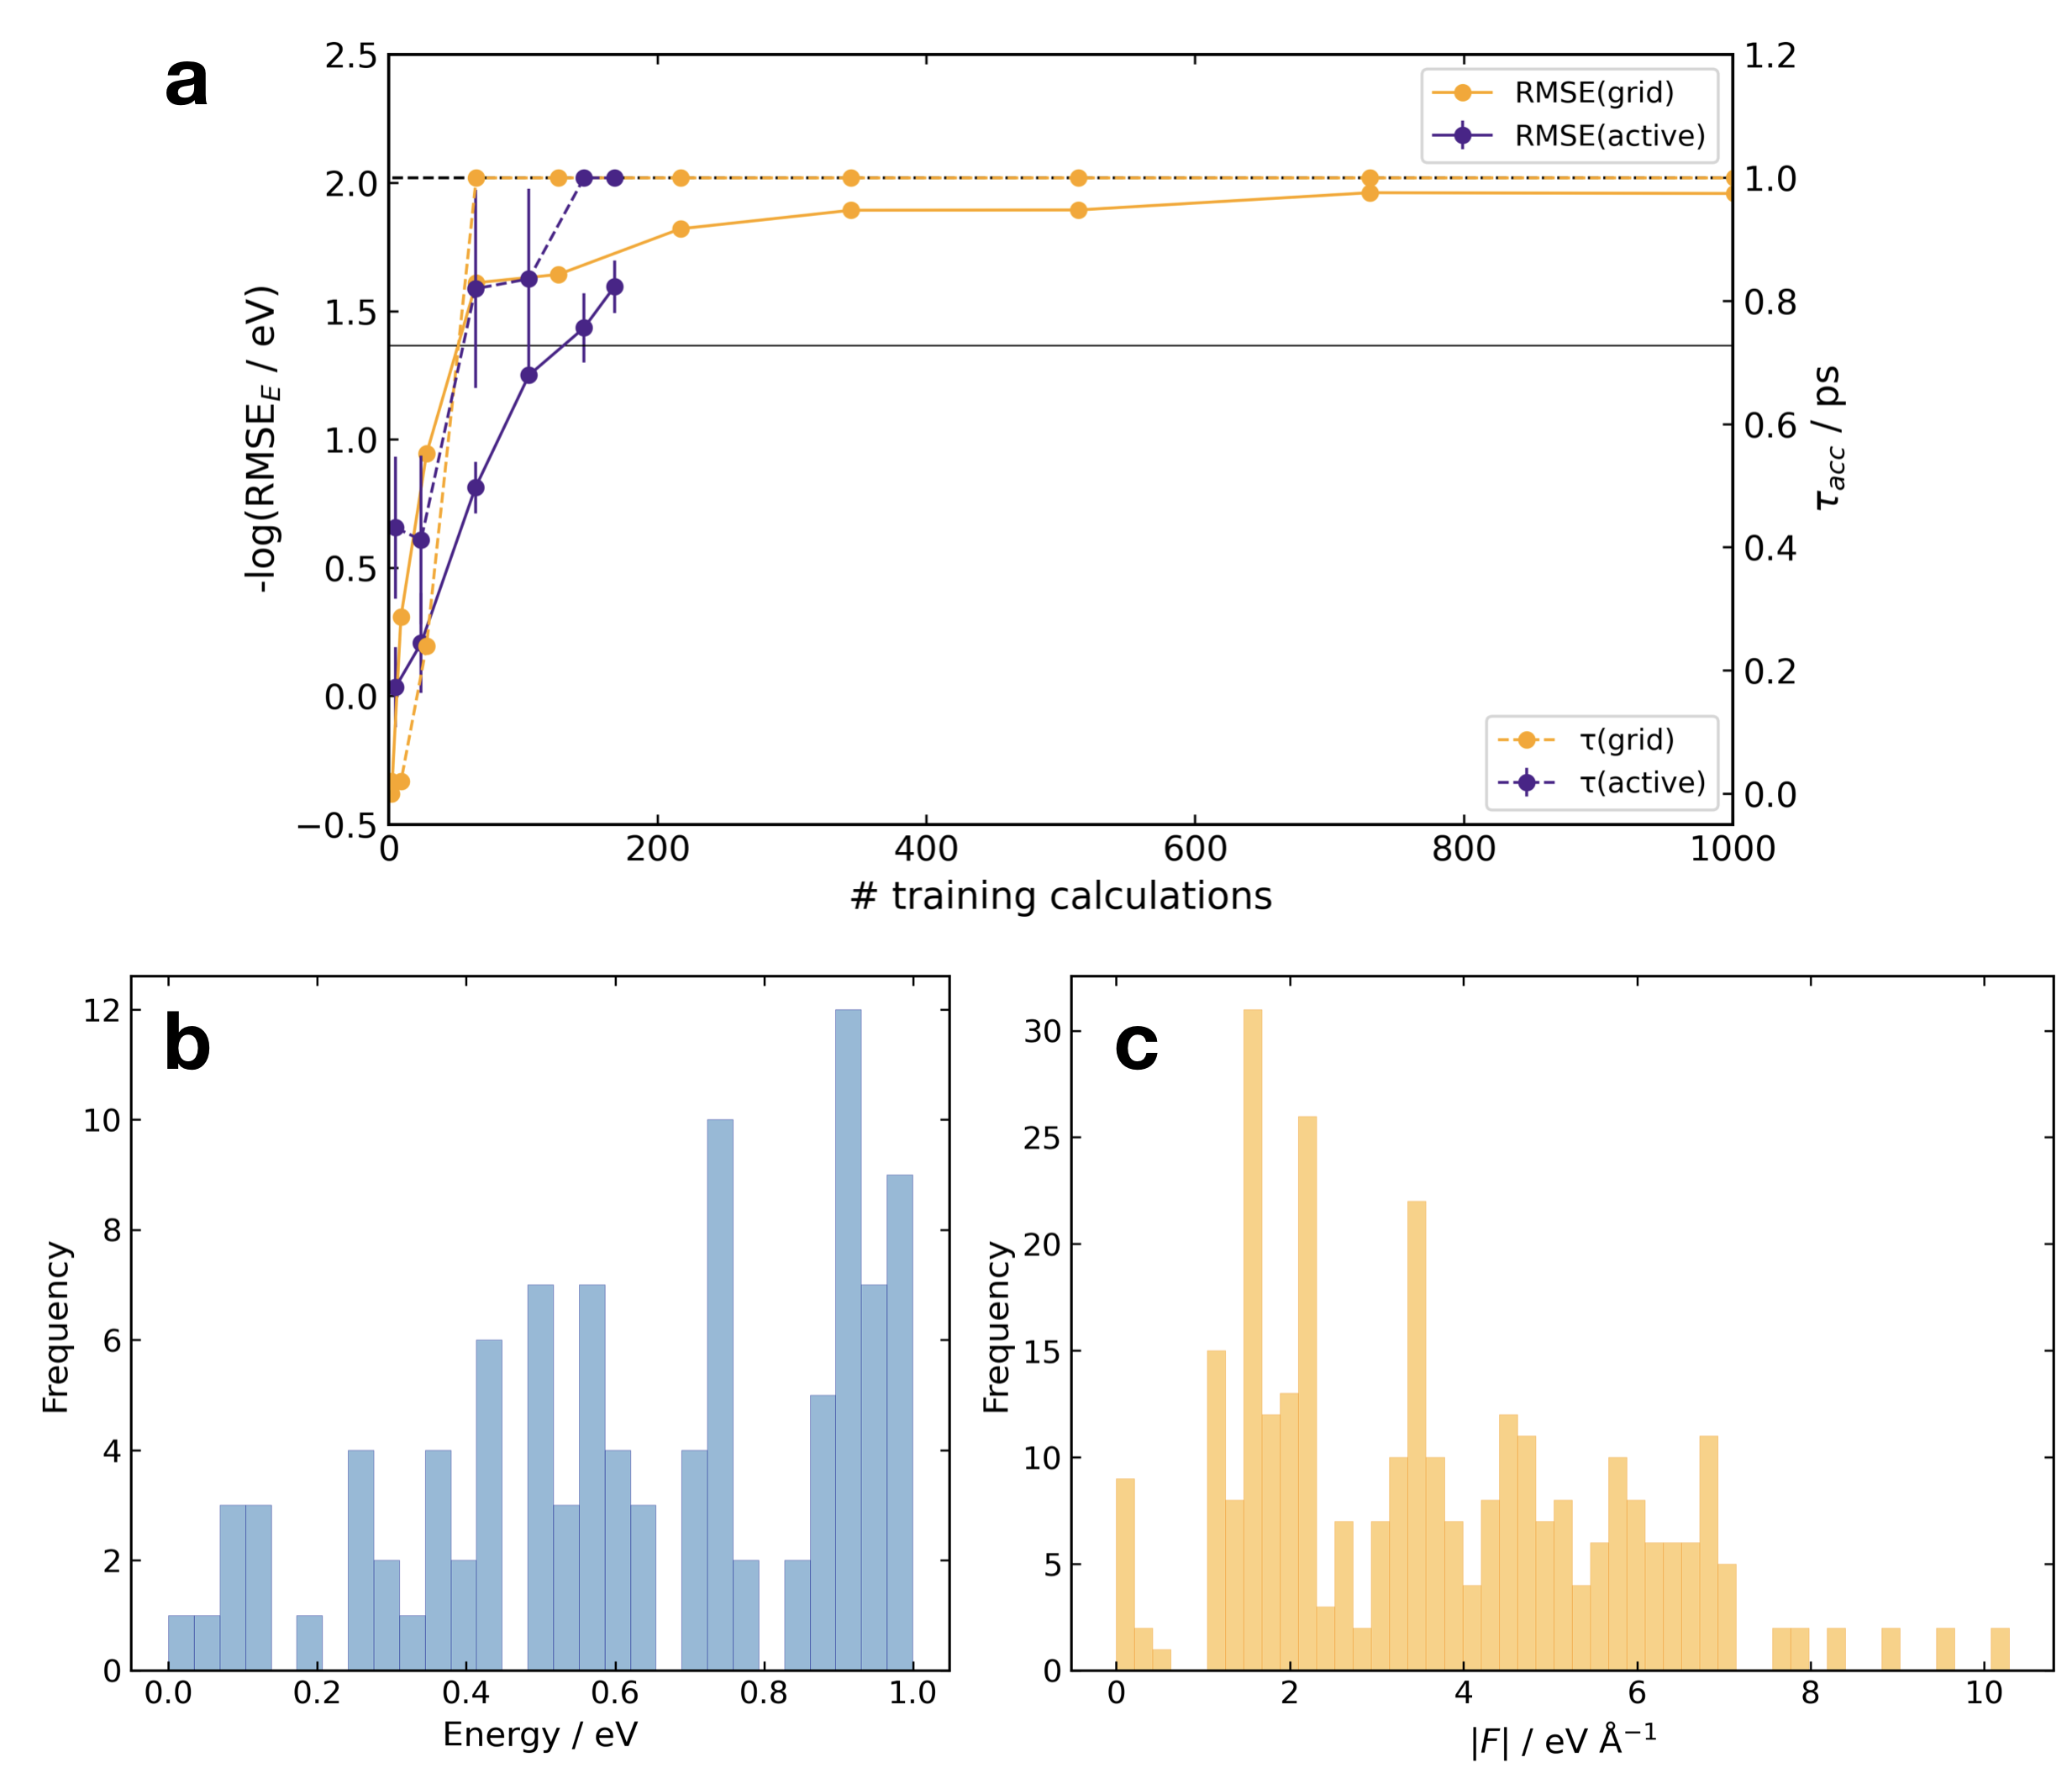
\includegraphics[width=\textwidth]{6/gap/figs_si/fig2}
	\vspace{0.2cm}
	\hrule
	\caption{(a) Comparison of active learning and a grid-based approach for training a water monomer. 2b+3b GAP with $r_c$ = 3.0 \AA without a SOAP all other parameters as P2 (Table \ref{table::ml_si_2}). $\max(\tau_\text{acc})$ = 1 ps calculated in a 2500 K simulation for a $\sim$1\% probability of accessing a configuration 1 eV above the minimum, $E_l$ = 0.043 eV, $E_T$ = 0.43 eV. (b, c) Energy and force distribution of the test data used to calculate a root mean squared error (RMSE) generated on a grid over $r_{\text{OH}_a}, r_{\text{OH}_b} \in [1.0, 1.3]$ \AA and $r_{\text{HH}} \in  [1.0, 2.5] $ \AA and truncated above 1 eV of the minimum to 103 data points that are not coincident with any training data.}
	\label{fig::ml_si_2}
\end{figure}


\begin{figure}[h!]
	\vspace{0.4cm}
	\centering
	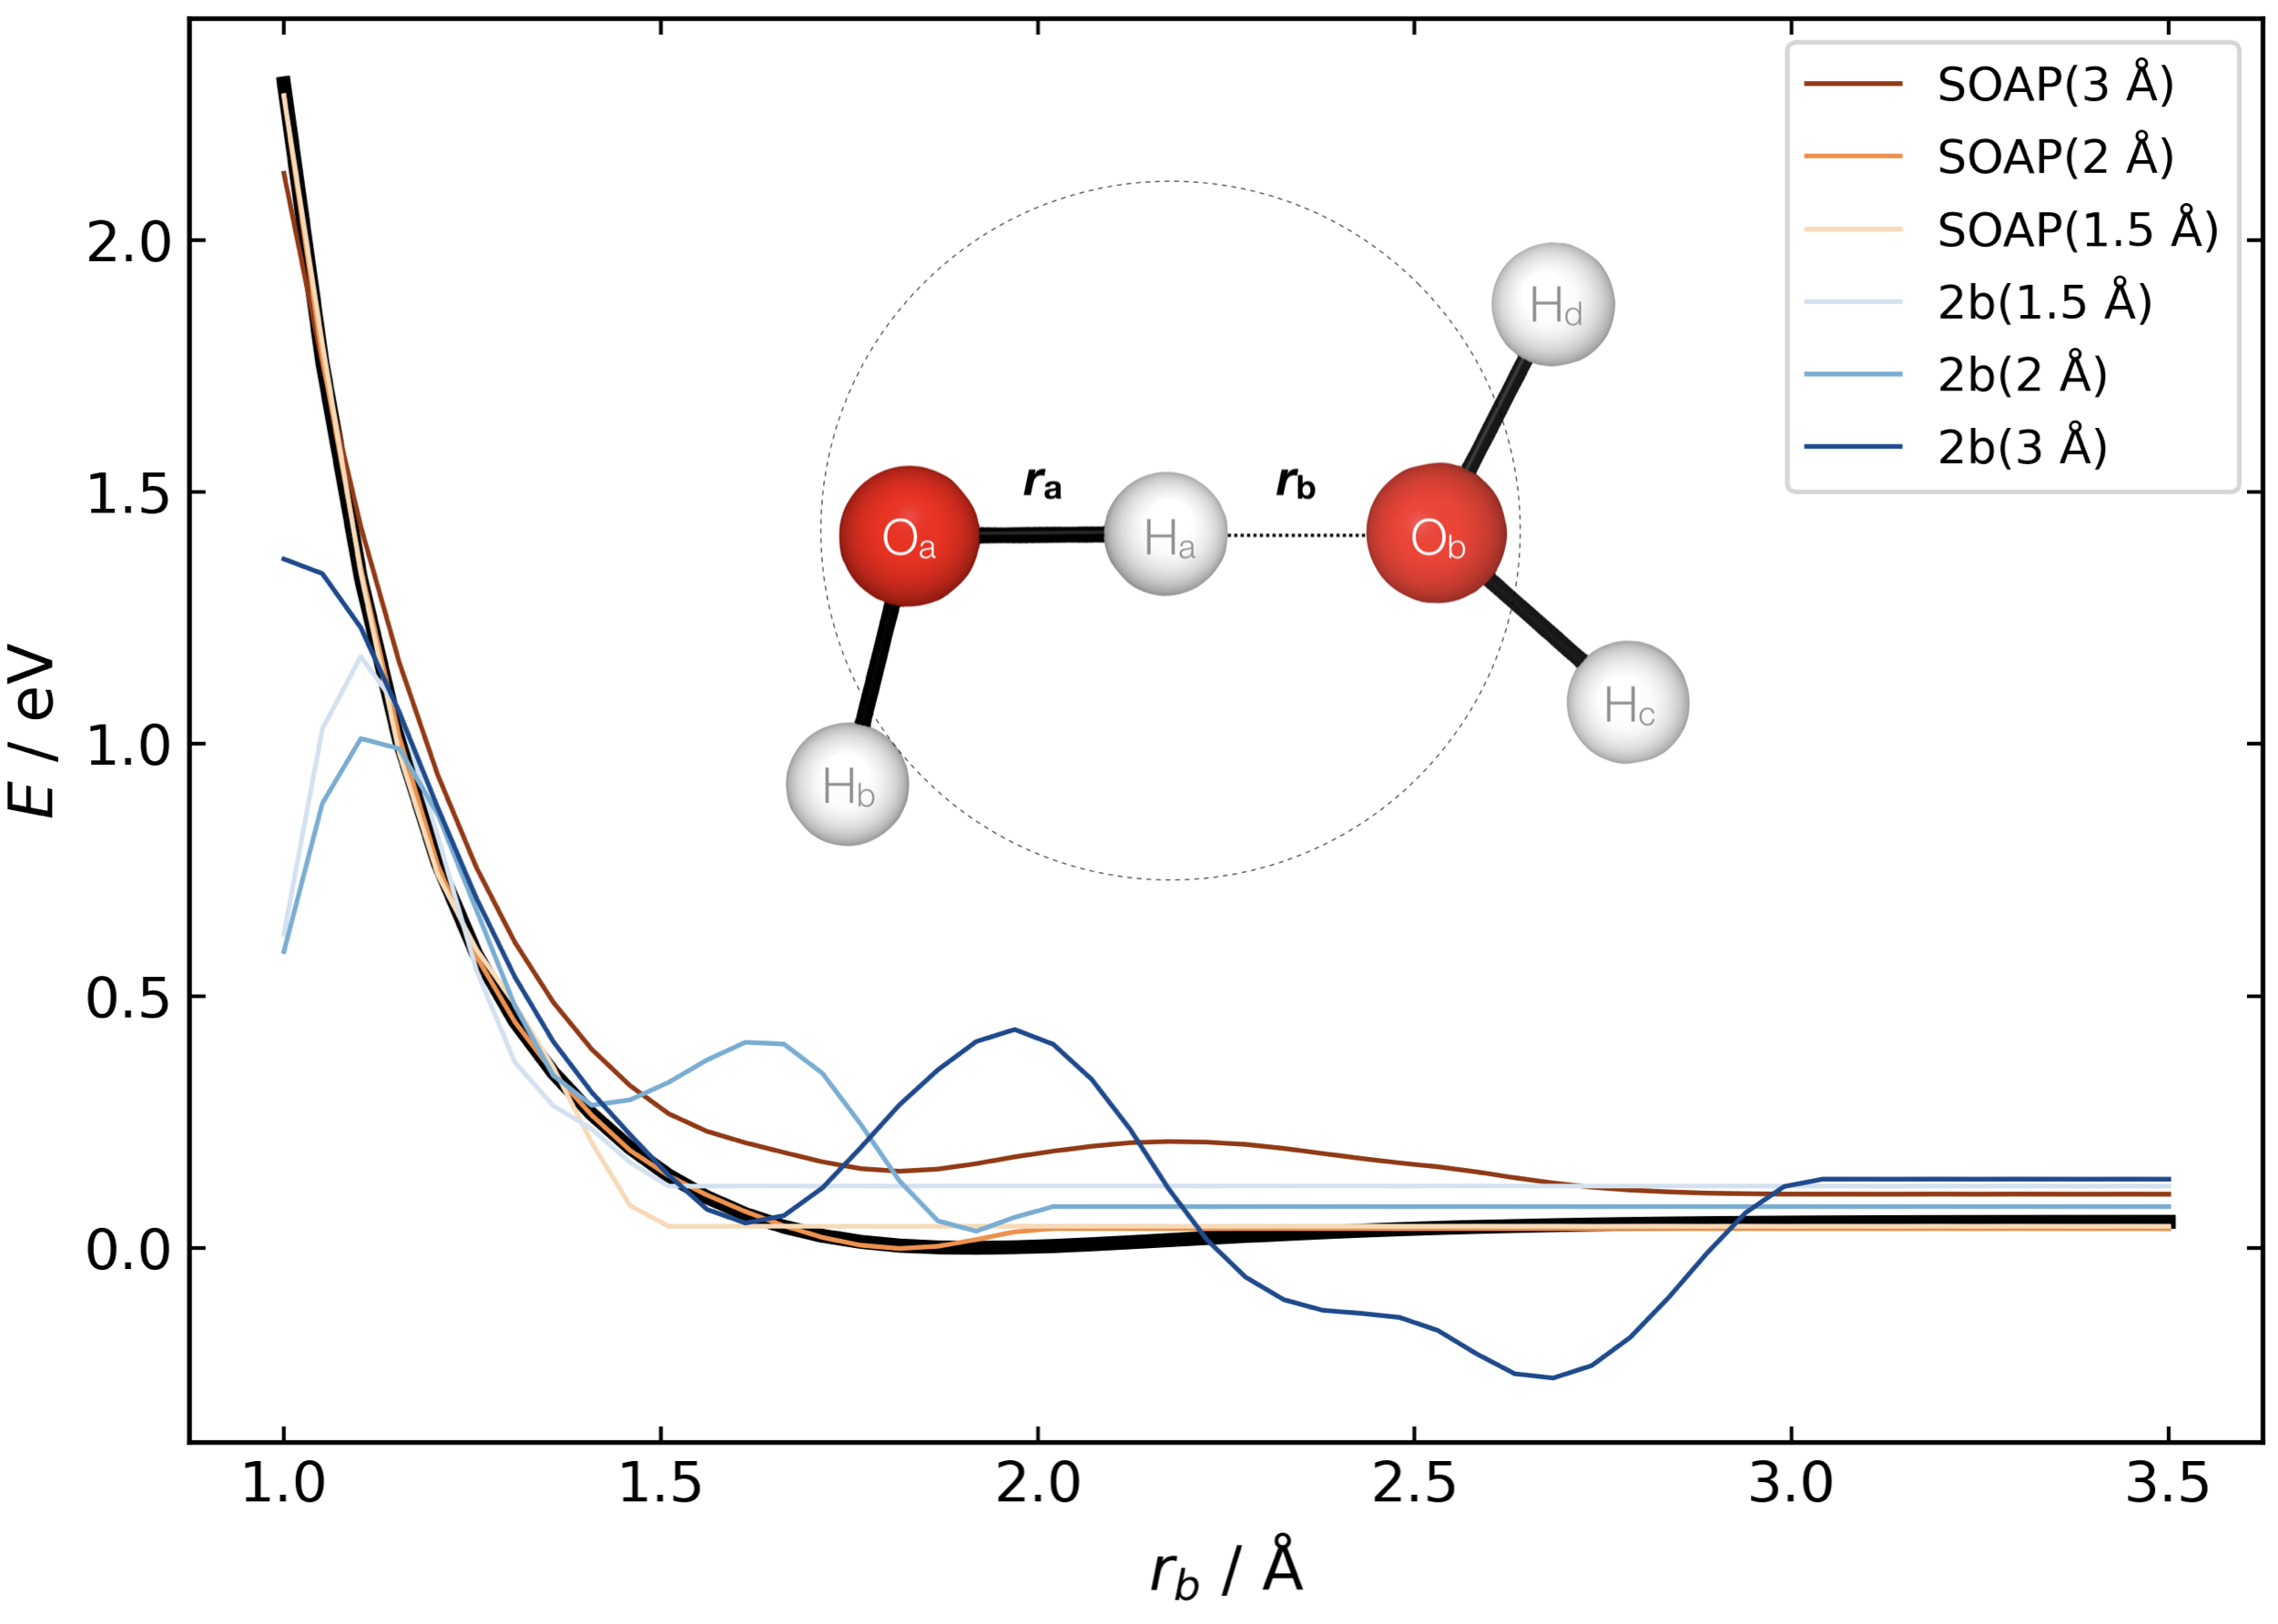
\includegraphics[width=10.5cm]{6/gap/figs_si/fig3}
	\vspace{0.2cm}
	\hrule
	\caption{Water dimer PES predicted using SOAP and 2b GAPs with the ground truth (DFTB(3ob)) in black. Trained on then evaluated on the PES points. Intramolecular component subtracted using the same intra-GAP as Figure 1 (2b+3b, $r_c$=3.0 \AA) evaluated in separate boxes.}
	\label{fig::ml_si_3}
\end{figure}


\begin{figure}[h!]
	\vspace{0.4cm}
	\centering
	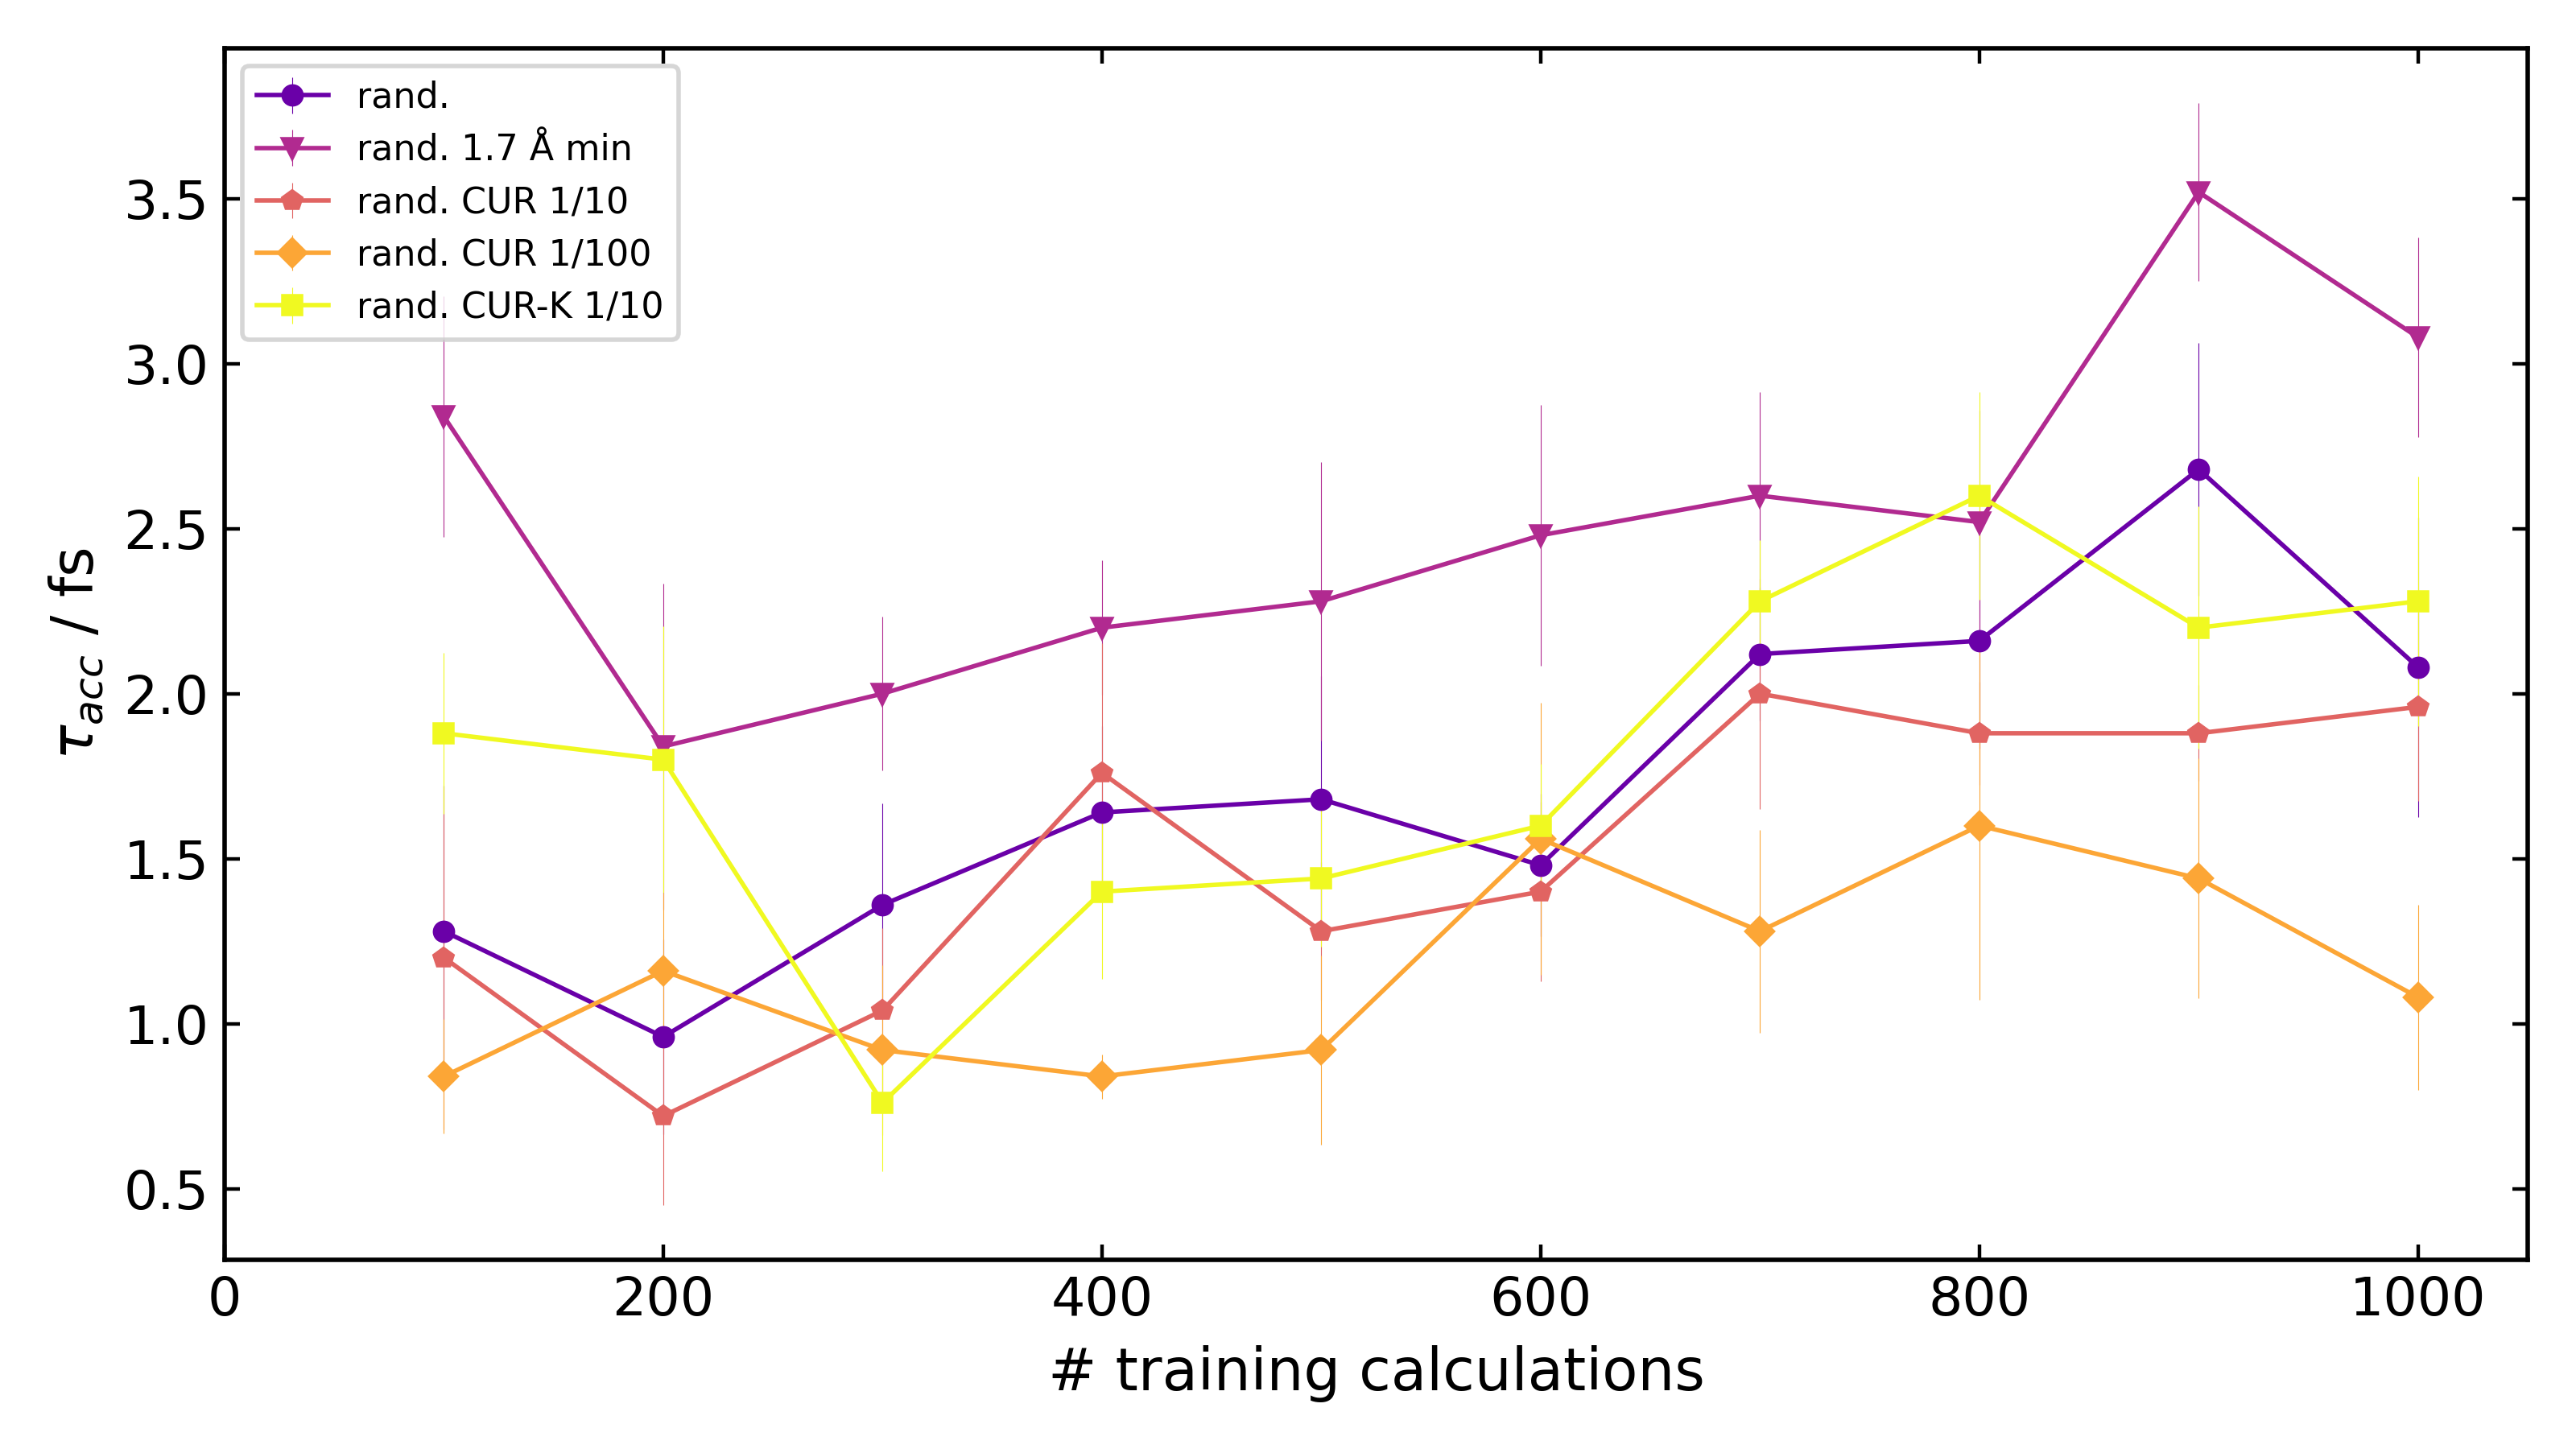
\includegraphics[width=13cm]{6/gap/figs_si/fig4}
	\vspace{0.2cm}
	\hrule
	\caption{Learning curves for a bulk water GAP trained on random configurations, with or without selection strategies. Water molecules randomized in the box by applying a random rotation and translation to each water molecule ensuring no intermolecular distance $<$ 1.5 \AA, apart from rand. 1.7 \AA min (purple triangles) where the minimum distance is 1.7 \AA. \taua calculated with a 1 fs interval, $E_l$ = 0.1 eV, $E_T$ = 1 eV averaged over 5 initial random configurations. Error bars are standard error in the mean over 5 independent iterations. CUR-K 1/10 is a CUR selection of the square kernel matrix between SOAP descriptors calculated using Dscribe,\cite{Himanen2020} keeping 1 in 10 rows, CUR is selection on the SOAP matrix averaged over atoms in the box.}
	\label{fig::ml_si_4}
\end{figure}


\begin{figure}[h!]
	\vspace{0.4cm}
	\centering
	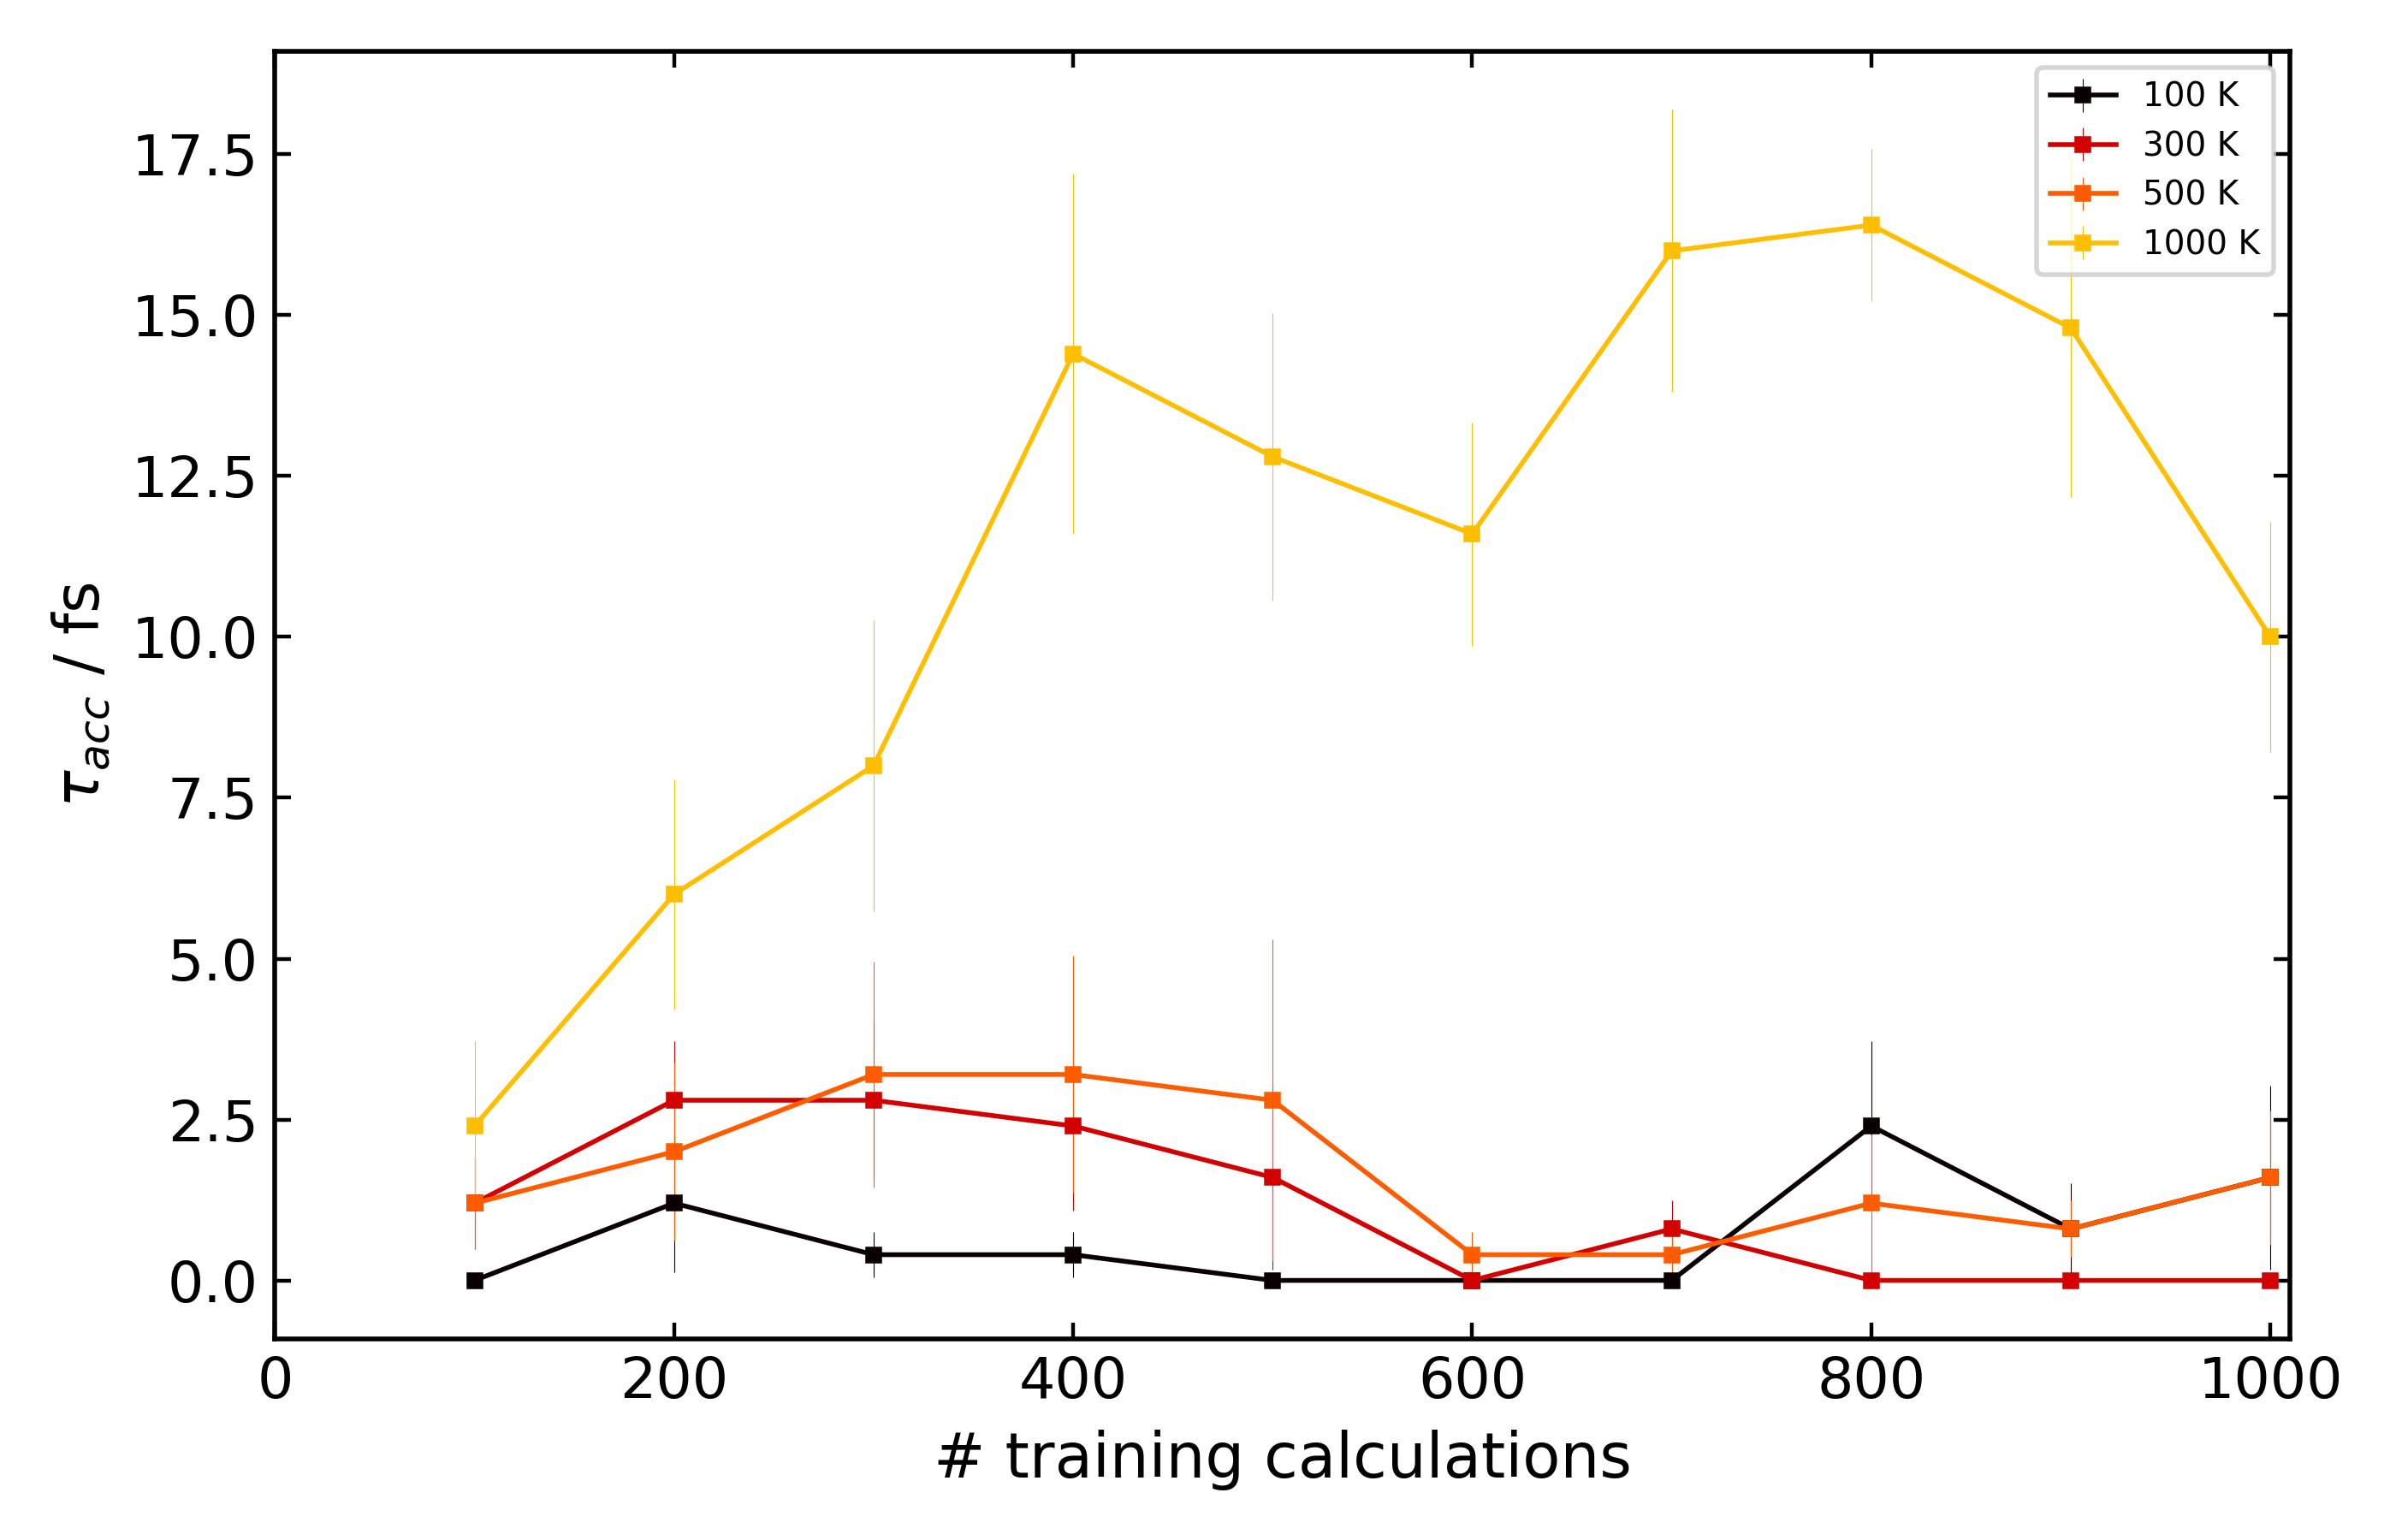
\includegraphics[width=12cm]{6/gap/figs_si/fig5}
	\vspace{0.2cm}
	\hrule
	\caption{Learning curves for a bulk water GAP trained on classical molecular mechanics configurations at different temperatures (performed by Tristan Johnston-Wood). Initial random configuration minimized then equilibrated for 1 ns, TIP3P parameters, flexible water. Configurations taken evenly spaced from a total of 10 ns of simulation time. \taua calculated with a 10 fs interval, $E_l$ = 0.1 eV, $E_T$ = 1 eV averaged over 5 initial random configurations. Error bars are standard error in the mean over 5 independent iterations.}
	\label{fig::ml_si_5}
\end{figure}



\begin{figure}[h!]
	\vspace{0.4cm}
	\centering
	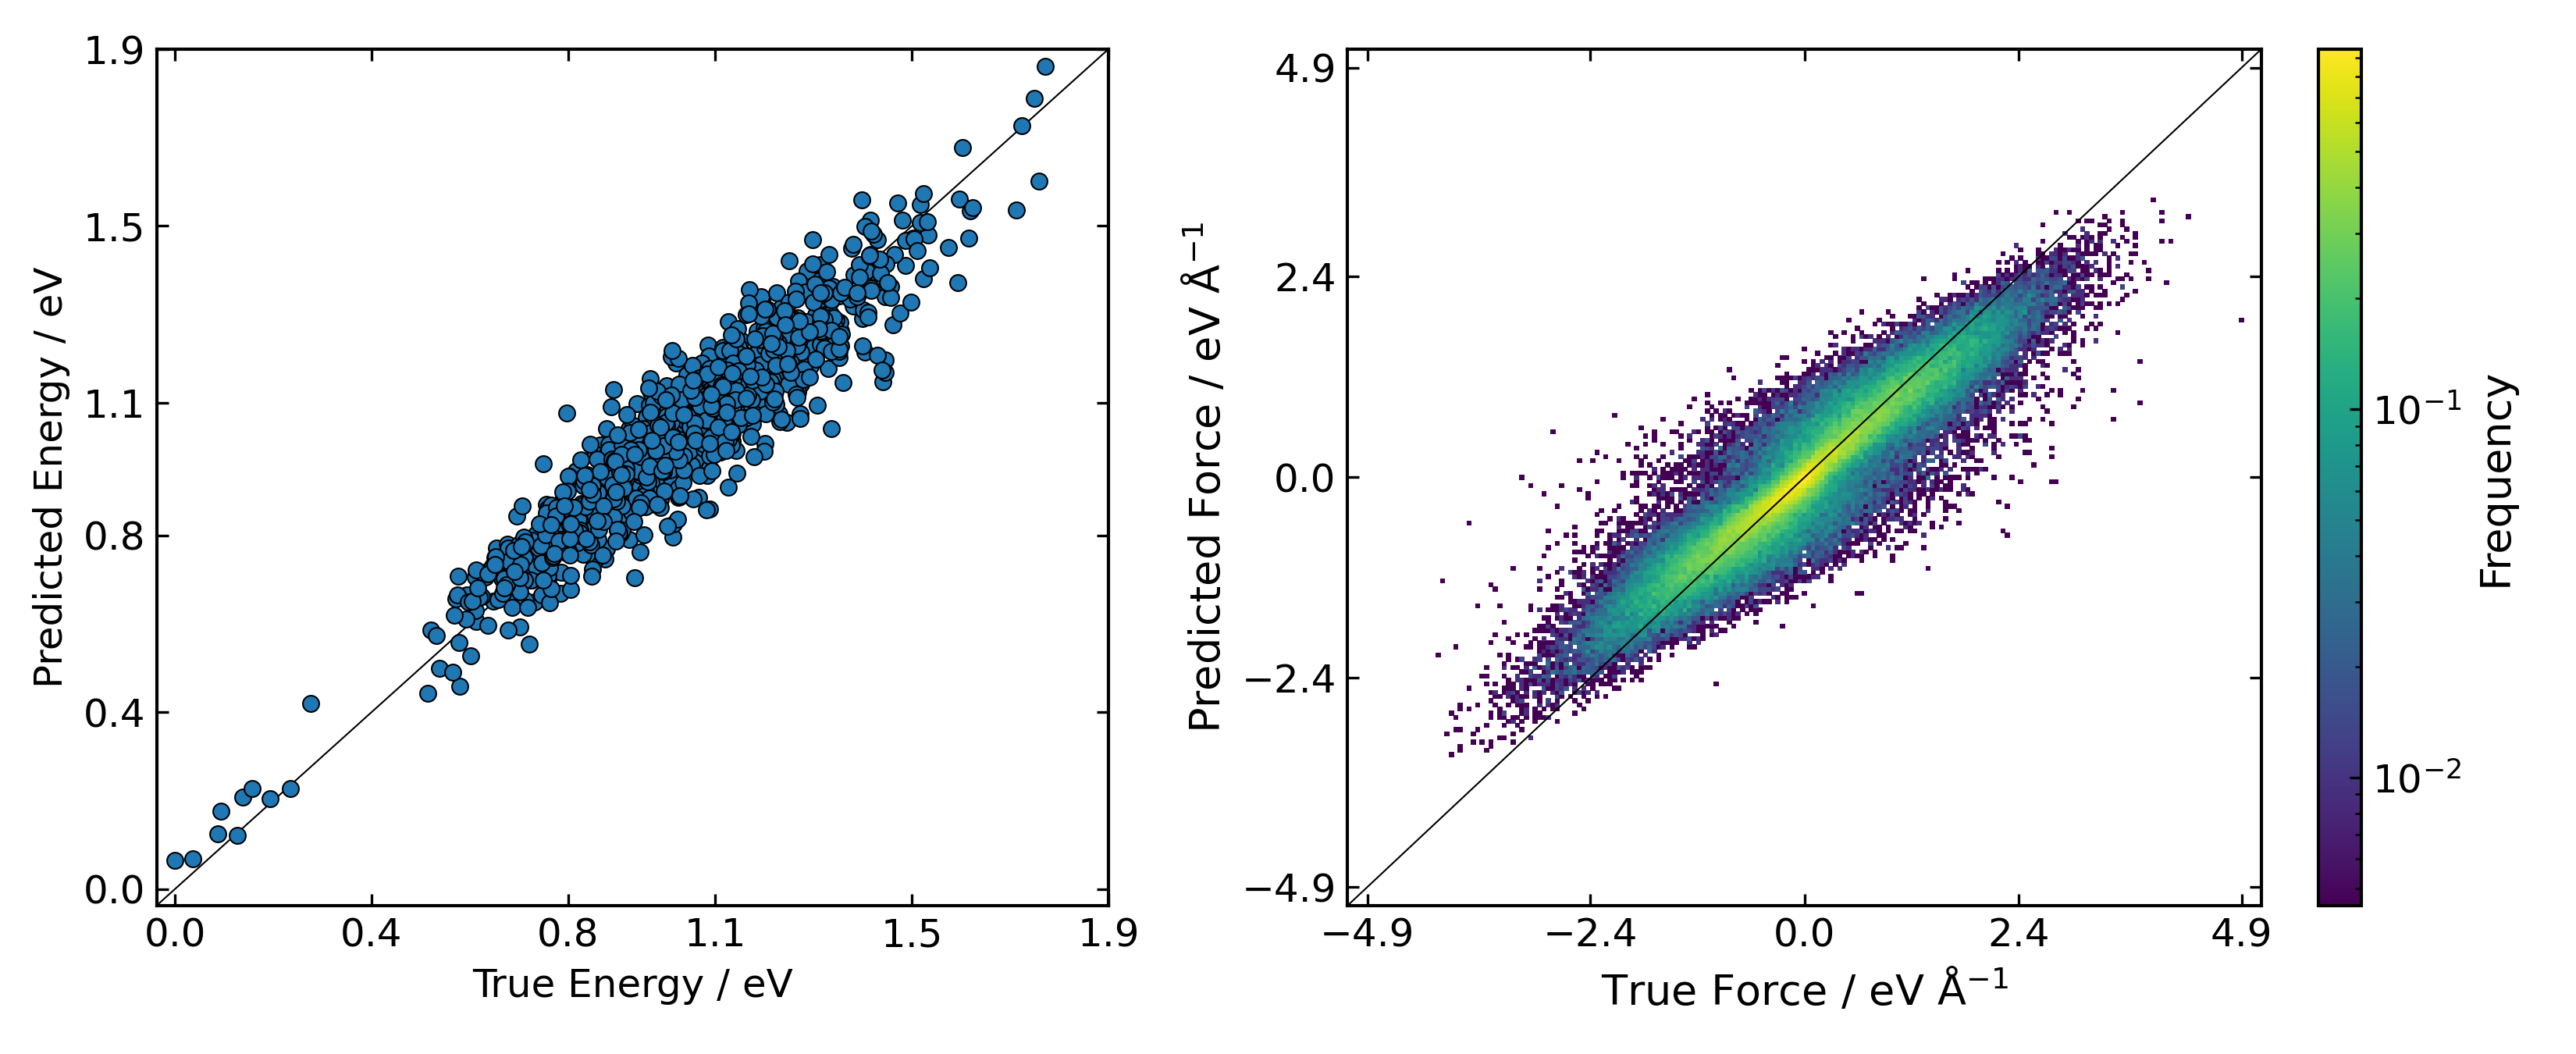
\includegraphics[width=\textwidth]{6/gap/figs_si/fig6}
	\vspace{0.2cm}
	\hrule
	\caption{Correlation plot between predicted and ‘true’ (DFTB) energies and forces on MM training data (300 K) for bulk water (TIP3P parameters).}
	\label{fig::ml_si_6}
\end{figure}



\begin{figure}[h!]
	\vspace{0.4cm}
	\centering
	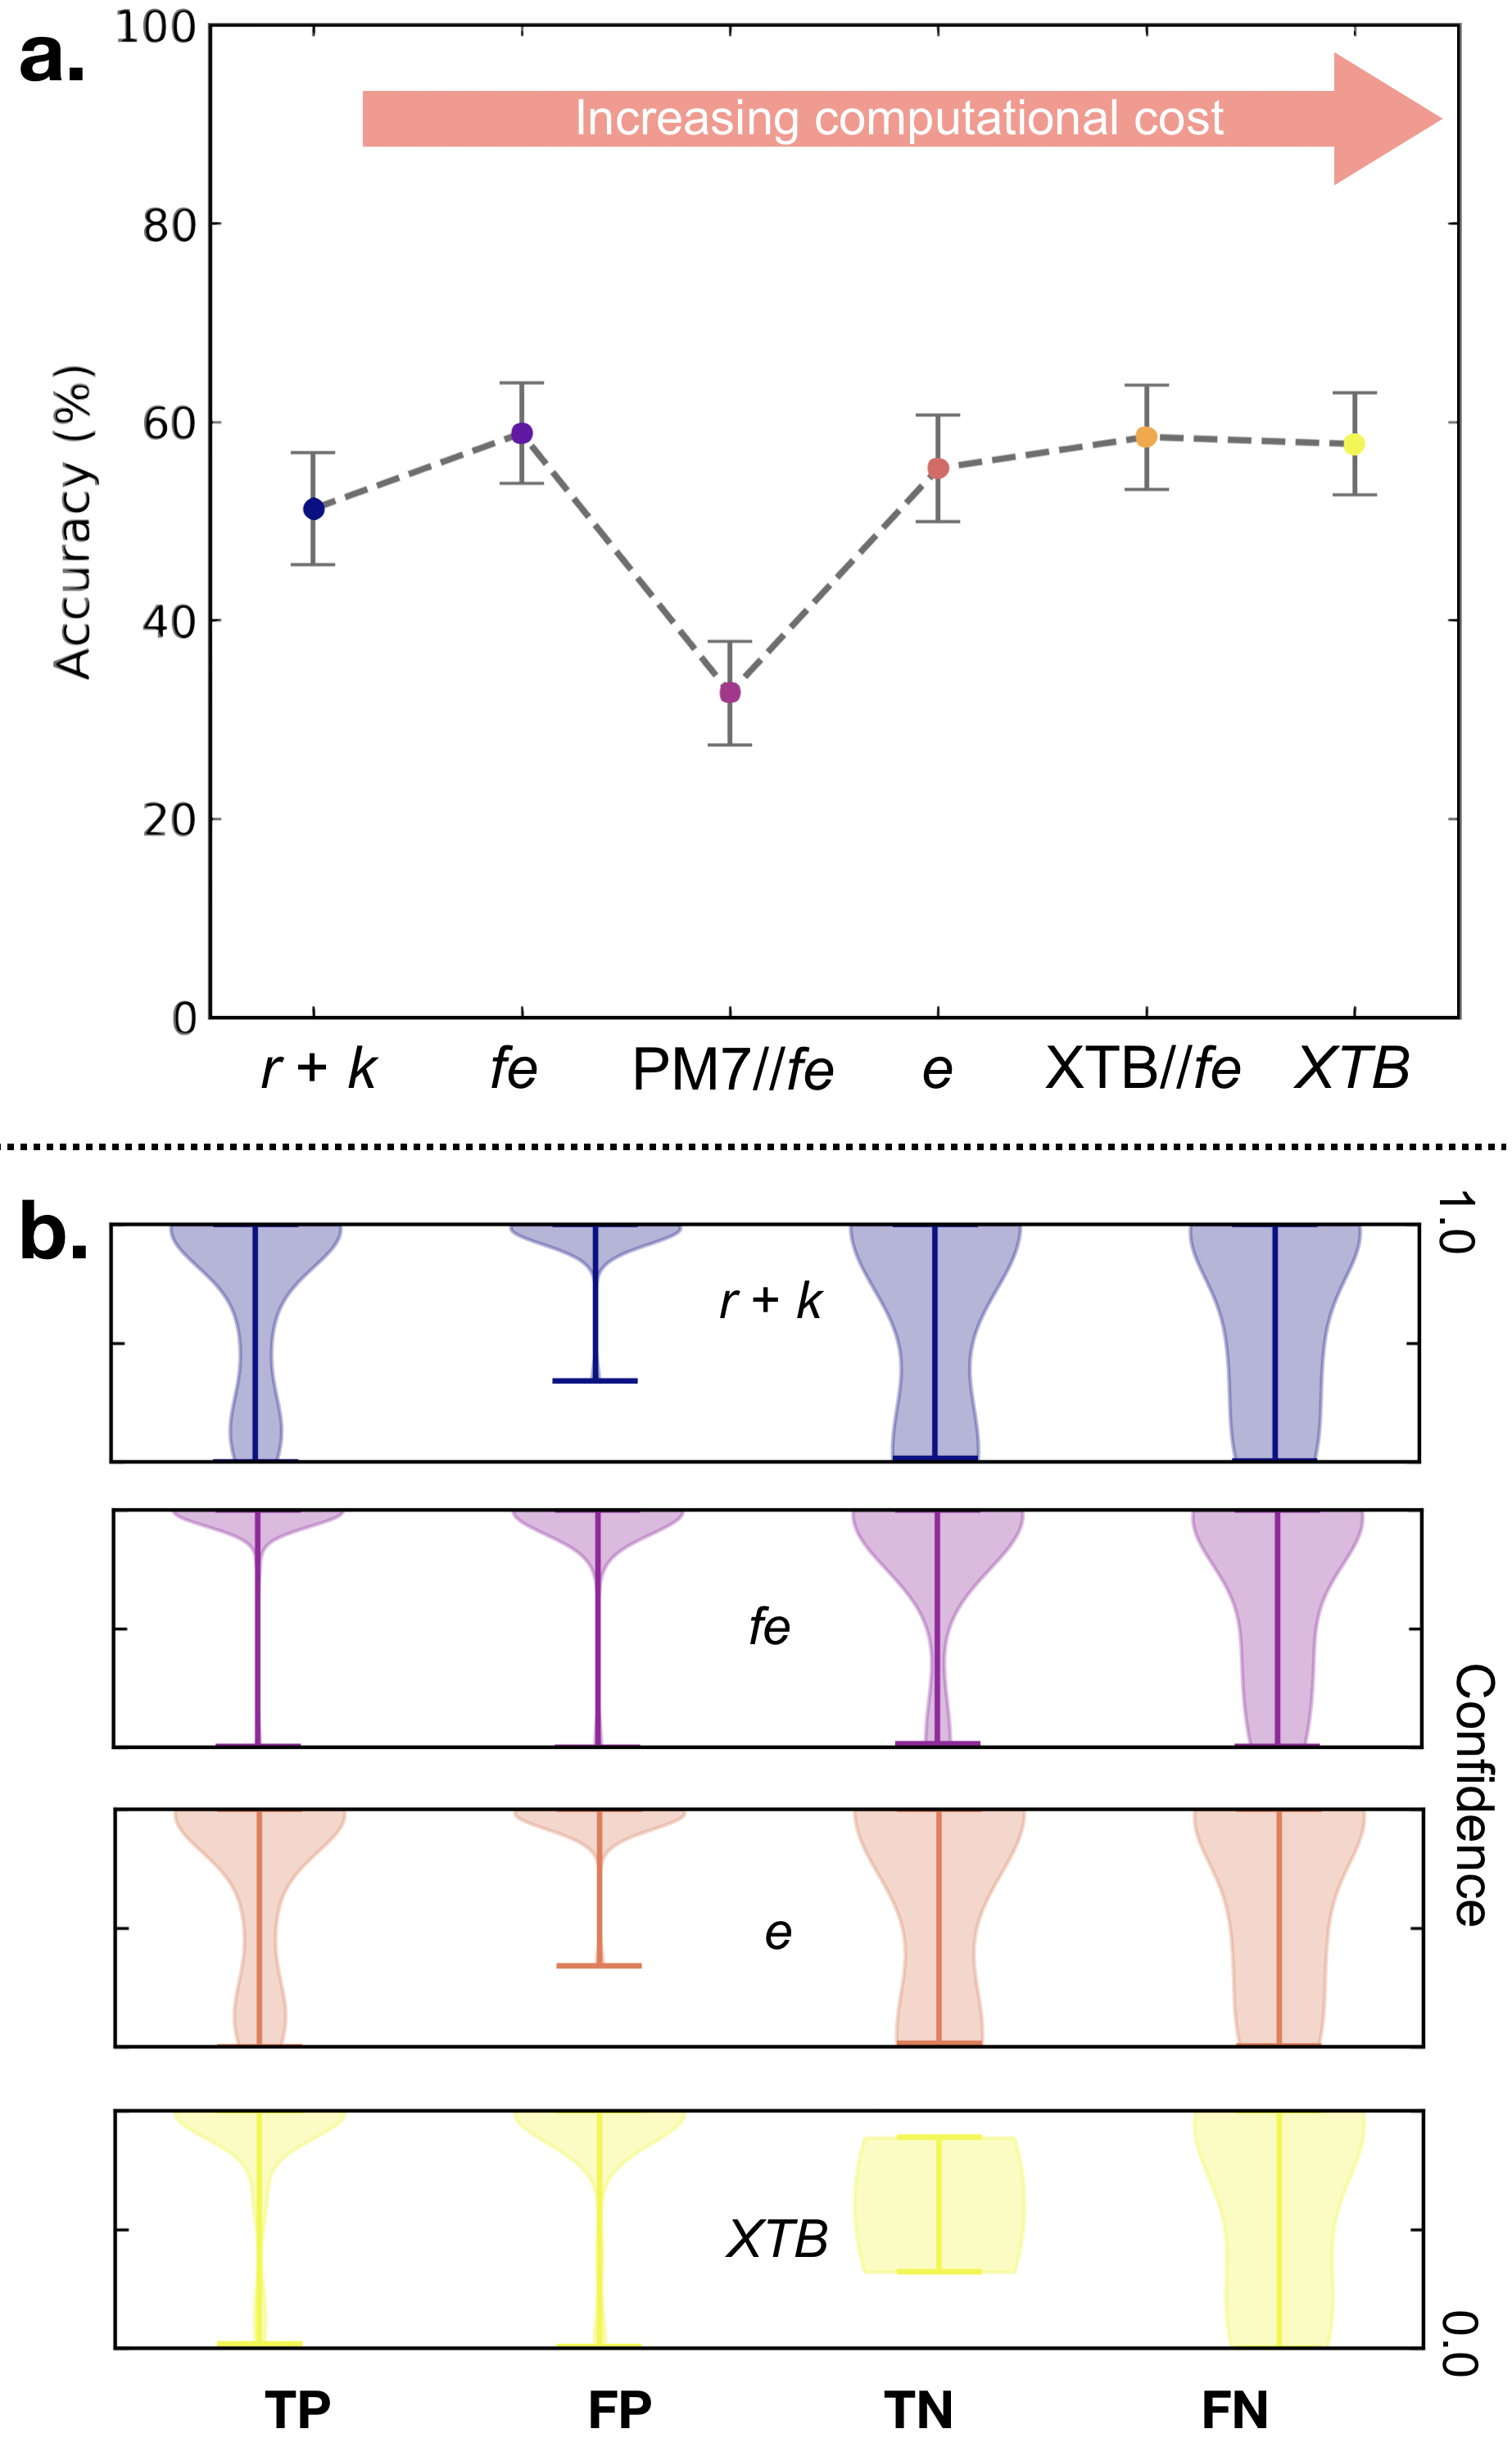
\includegraphics[width=\textwidth]{6/gap/figs_si/fig7}
	\vspace{0.2cm}
	\hrule
	\caption{Kernel matrices on normalised SOAP vectors between MM-MD and AIMD frames simulated at 300 K calculated using Dscribe,\cite{Himanen2020} with ‘inner’ averaging (average coefficients over sites before summation over angular projection, m) over unique elements (H, O), $r_c$ = 5 \AA, $n_\text{max}=l_\text{max}=6$, raised to the 4th power (i.e.$\zeta=4$). Values 0--1 correspond to minimal–maximal similarity in configurations.}
	\label{fig::ml_si_7}
\end{figure}




\begin{figure}[h!]
	\vspace{0.4cm}
	\centering
	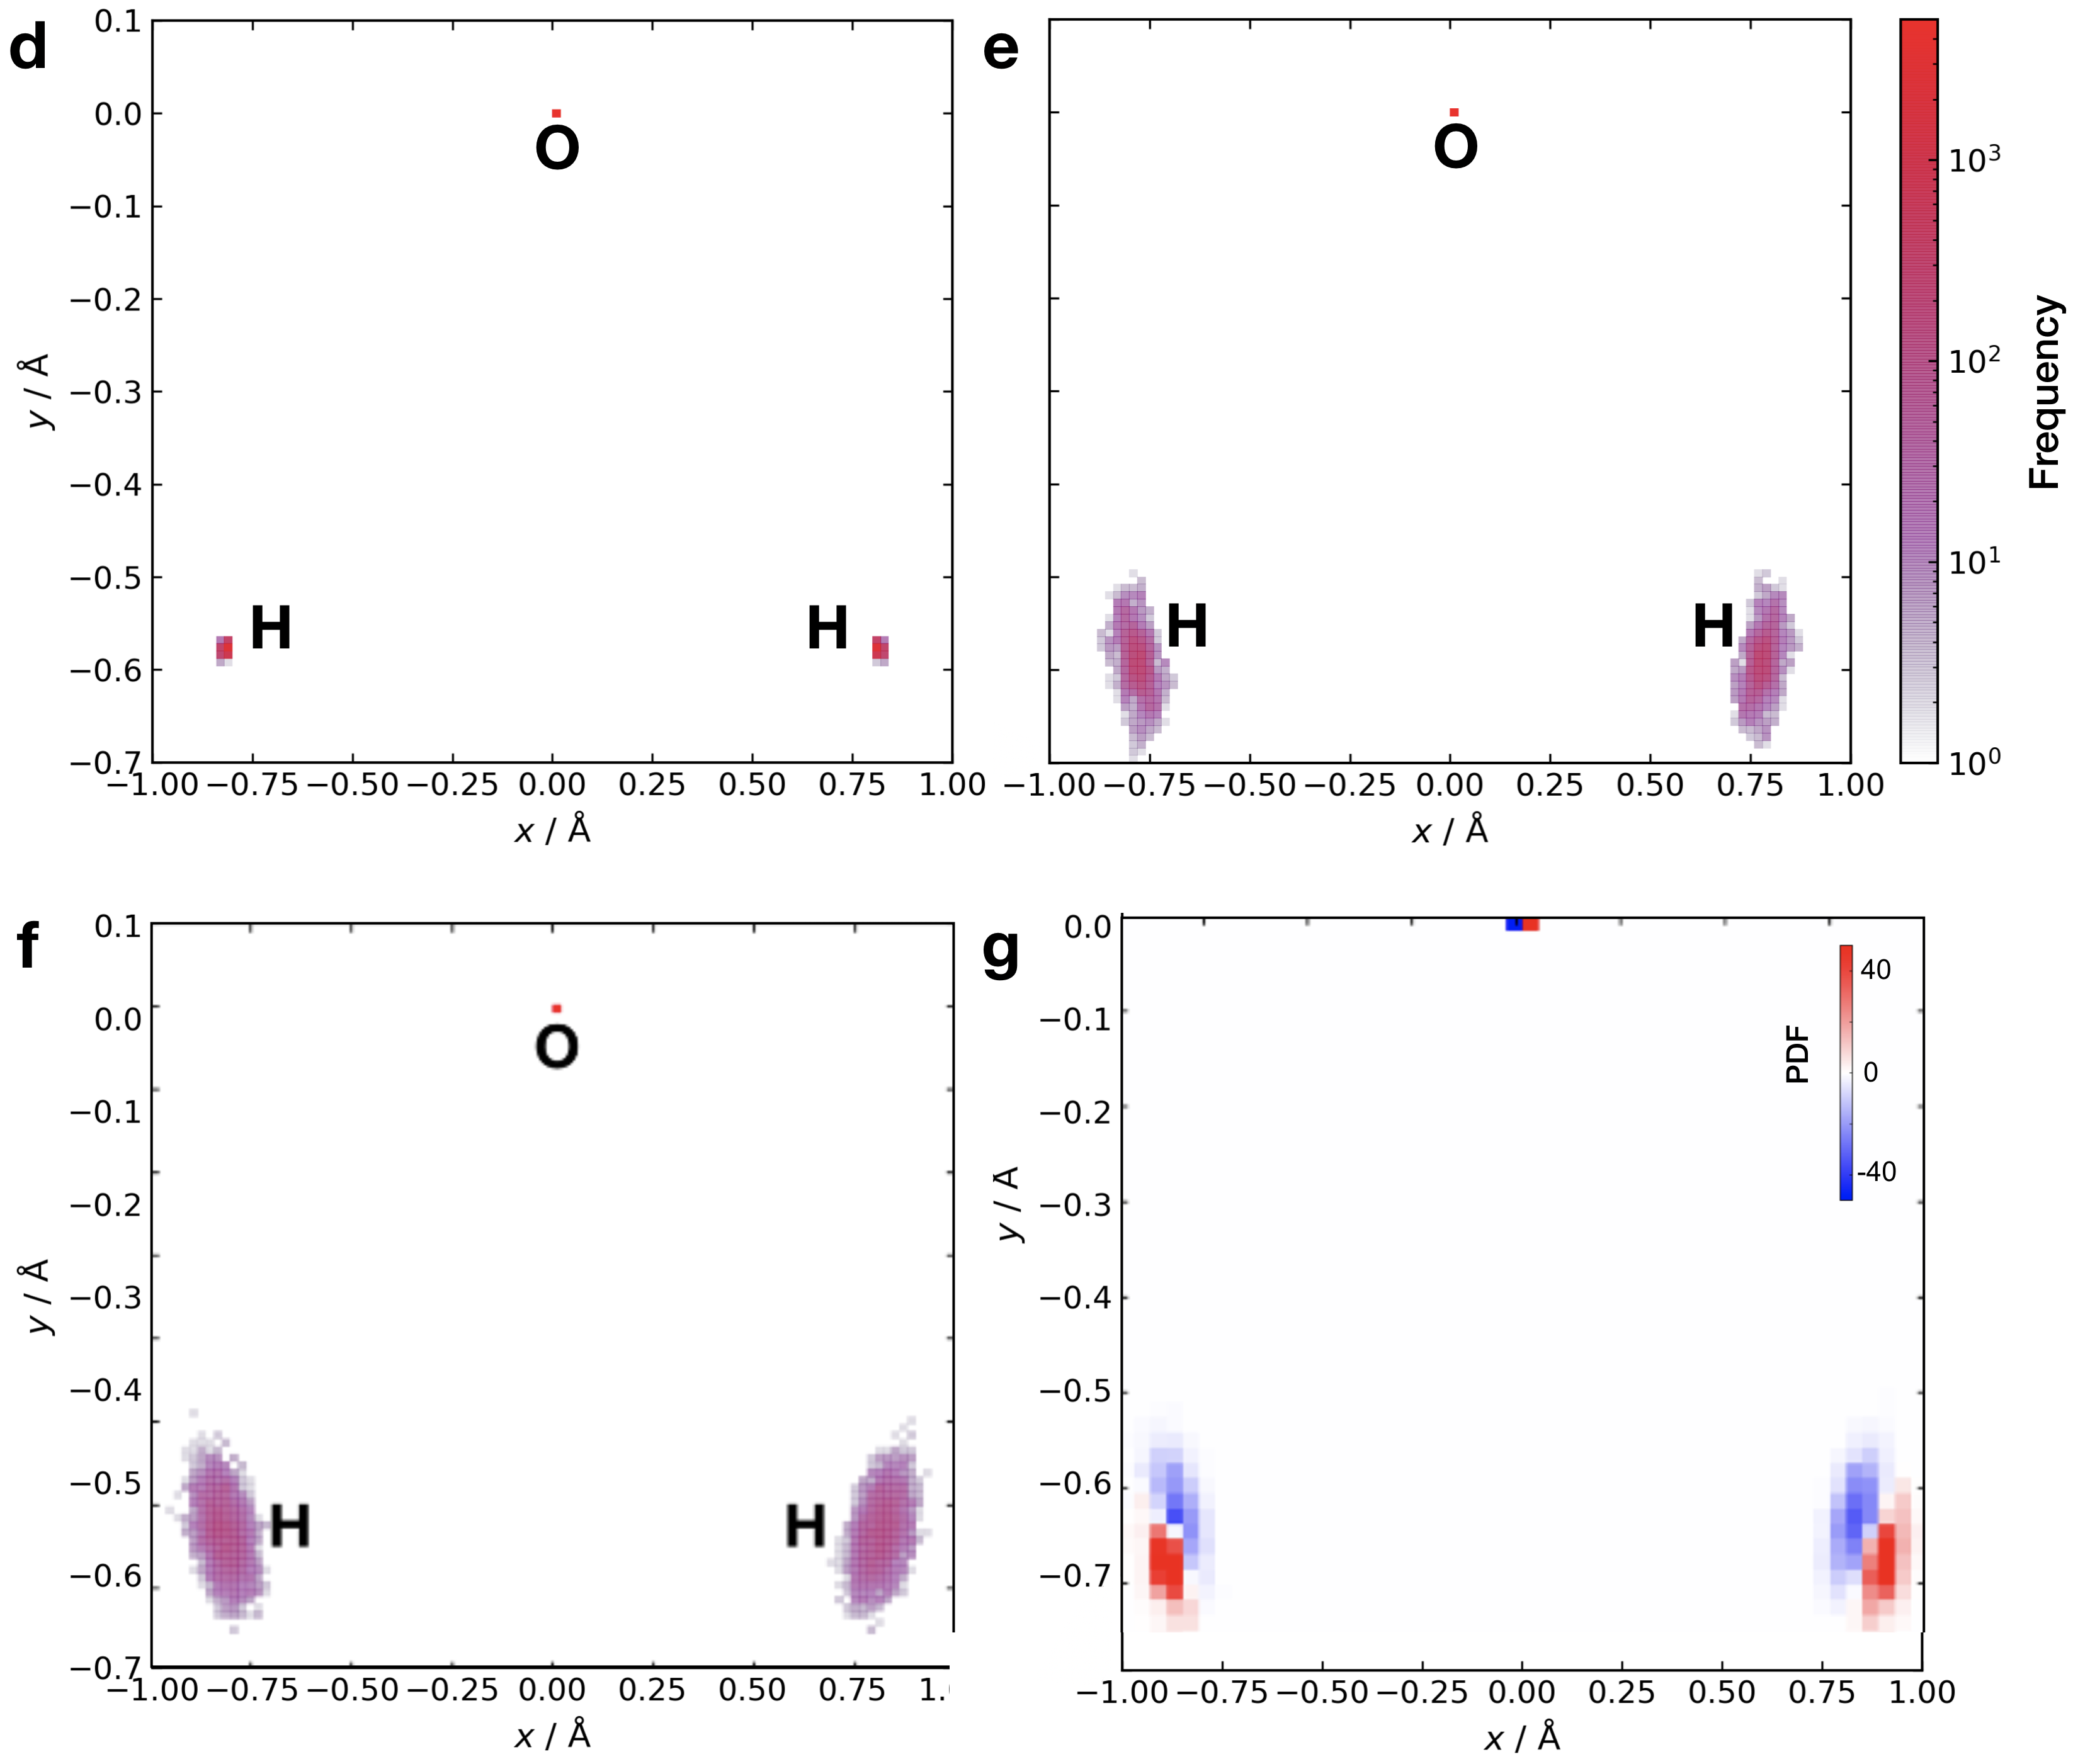
\includegraphics[width=\textwidth]{6/gap/figs_si/fig7cont}
	\vspace{0.2cm}
	\hrule
	\caption{Figure \ref{fig::ml_si_6} continued. Histogram of atomic positions in (d) MM(TIP3P) with LINCS H-constraints and without (f), (e) AIMD(DFTB) configurations generated over a 300 K trajectory and the difference between MM(ITIP3P, no LINCS) and AIMD (g). All water molecules fitted to an initial reference in the xy plane with the Kabash algorithm, oxygen centred at (0, 0). Only molecules wholly within the box included.}
	\label{fig::ml_si_7cont}
\end{figure}





\begin{figure}[h!]
	\vspace{0.4cm}
	\centering
	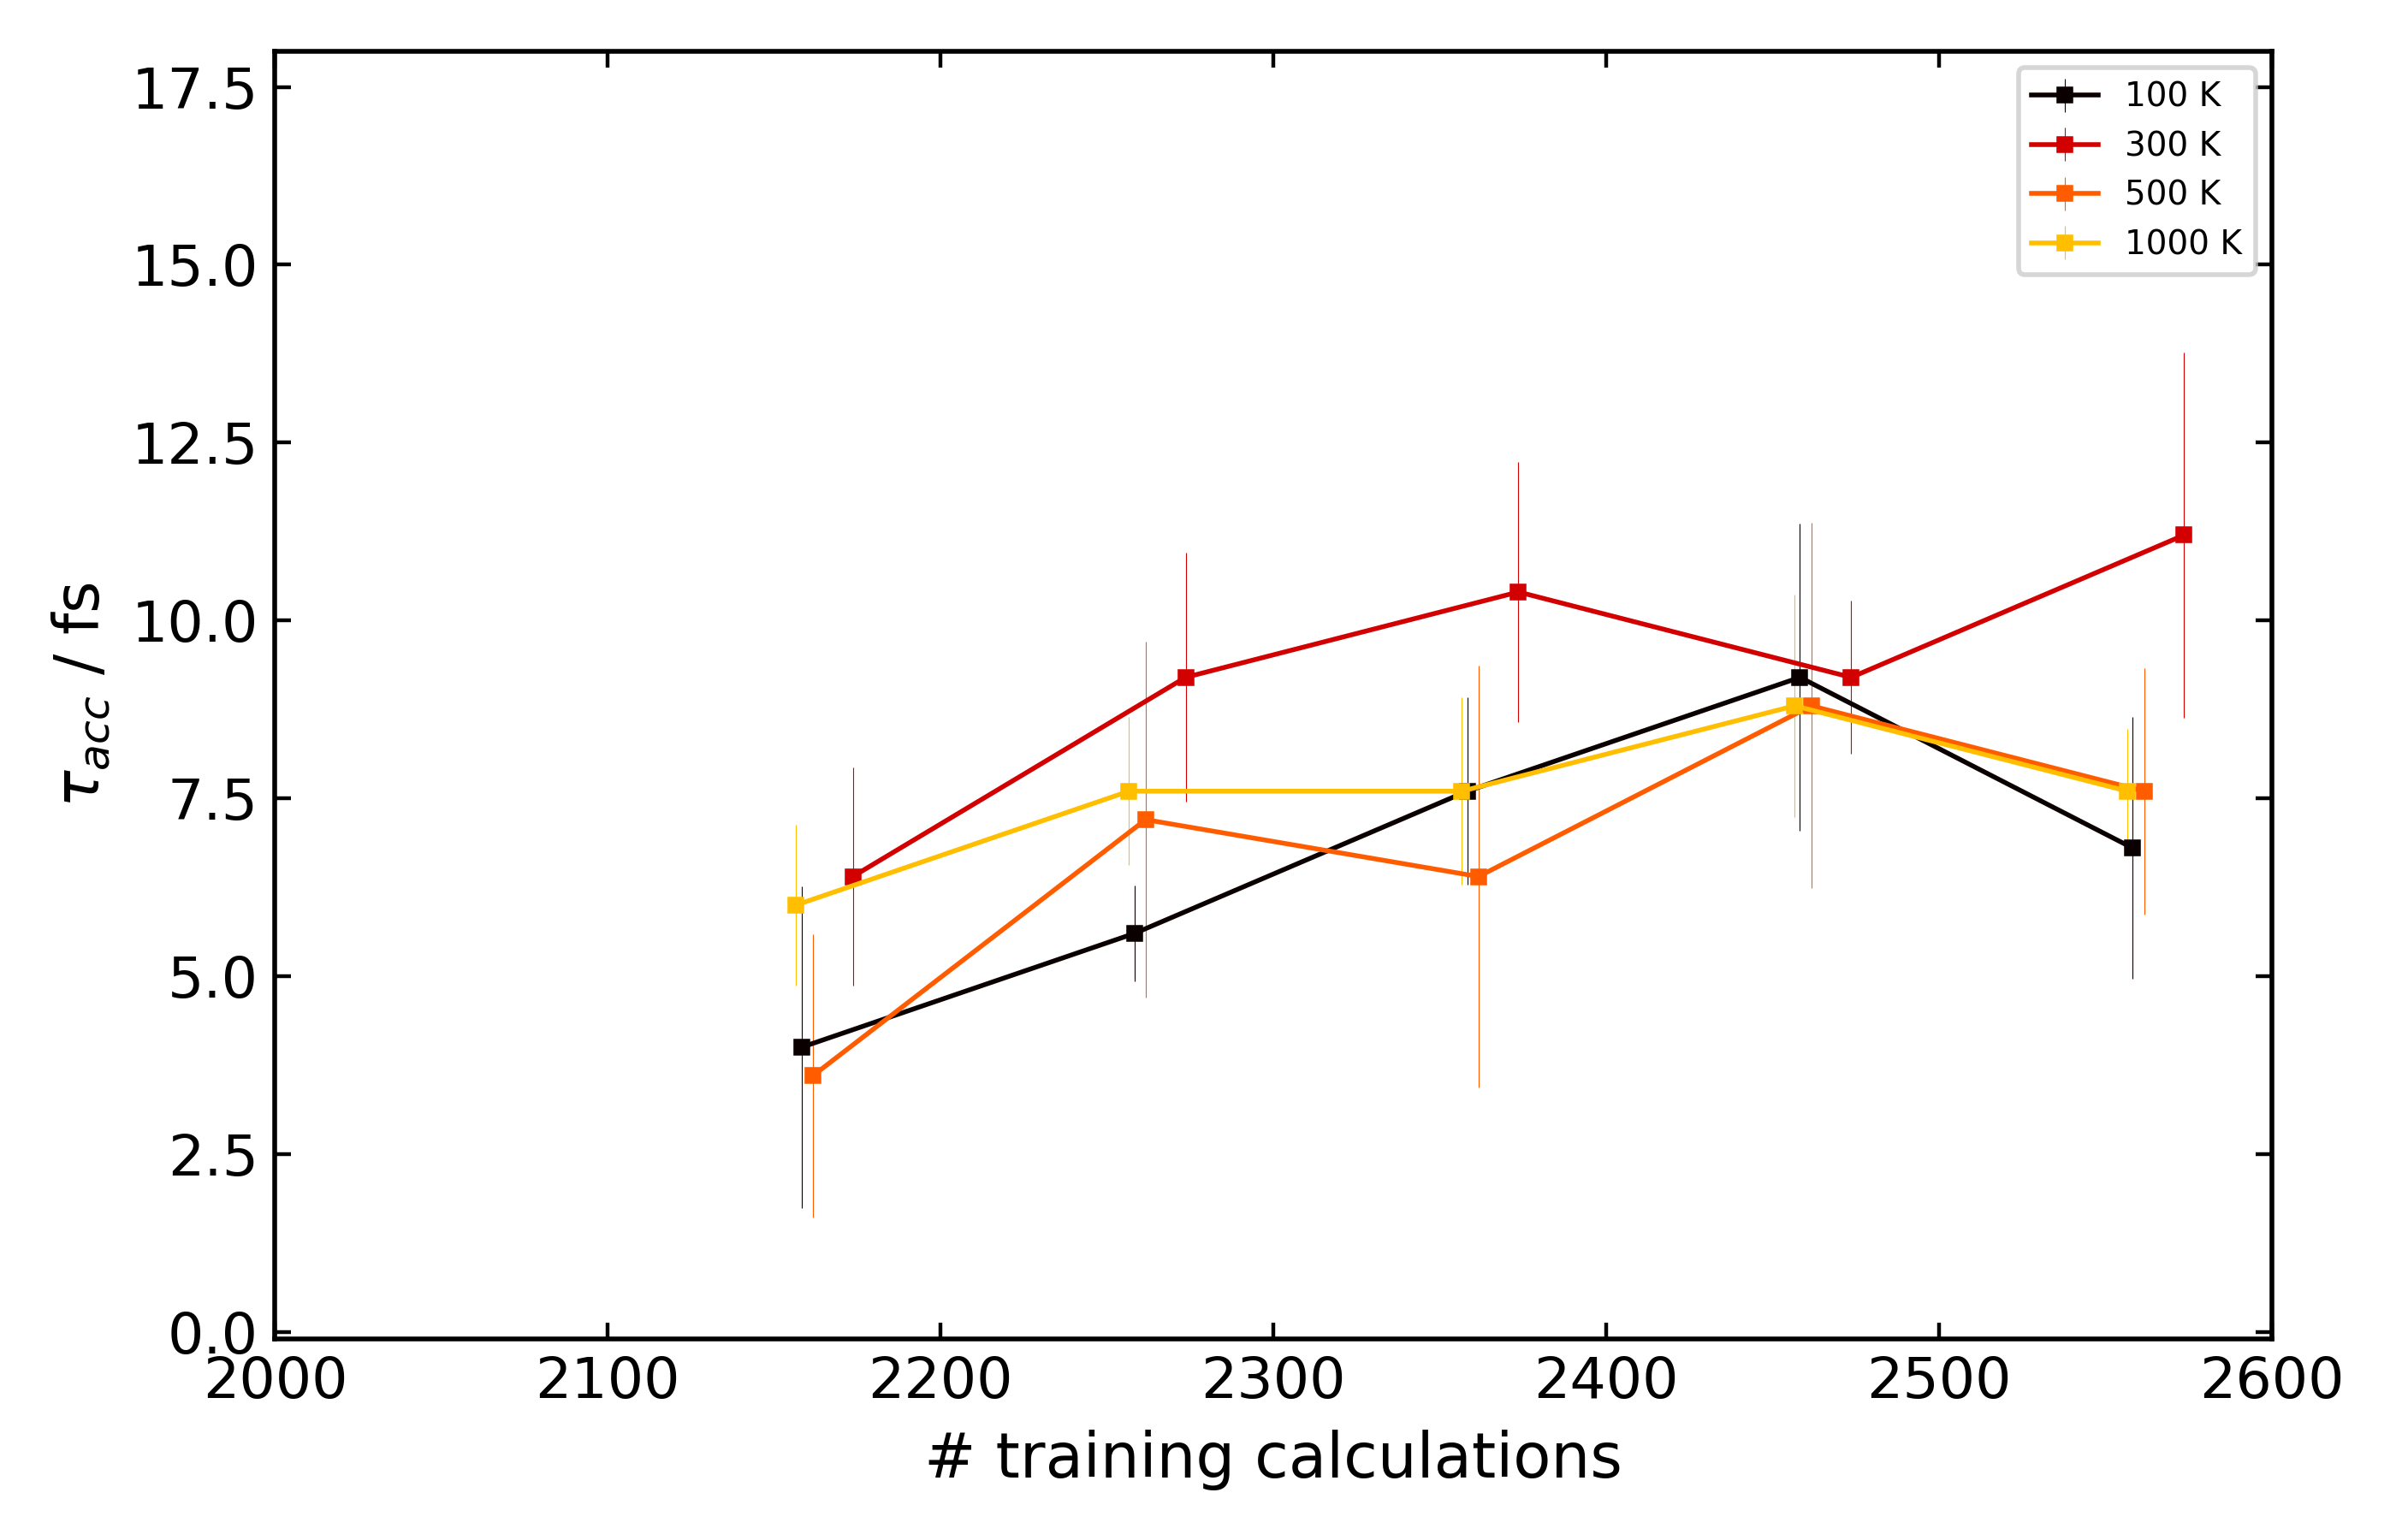
\includegraphics[width=11.5cm]{6/gap/figs_si/fig8}
	\vspace{0.2cm}
	\hrule
	\caption{Learning curves for a bulk water GAP trained on classical ‘ab-initio’ [AIMD, DFTB(3ob)] configurations at different temperatures.  Initial random configuration minimized at DFTB. Configurations taken evenly spaced from a total of 1 ps of simulation time. \taua calculated with a 10 fs interval, $E_l$ = 0.1 eV, $E_T$ = 1 eV averaged over 5 initial random configurations. Error bars are standard error in the mean over 5 independent iterations.}
	\label{fig::ml_si_8}
\end{figure}



\begin{figure}[h!]
	\vspace{0.4cm}
	\centering
	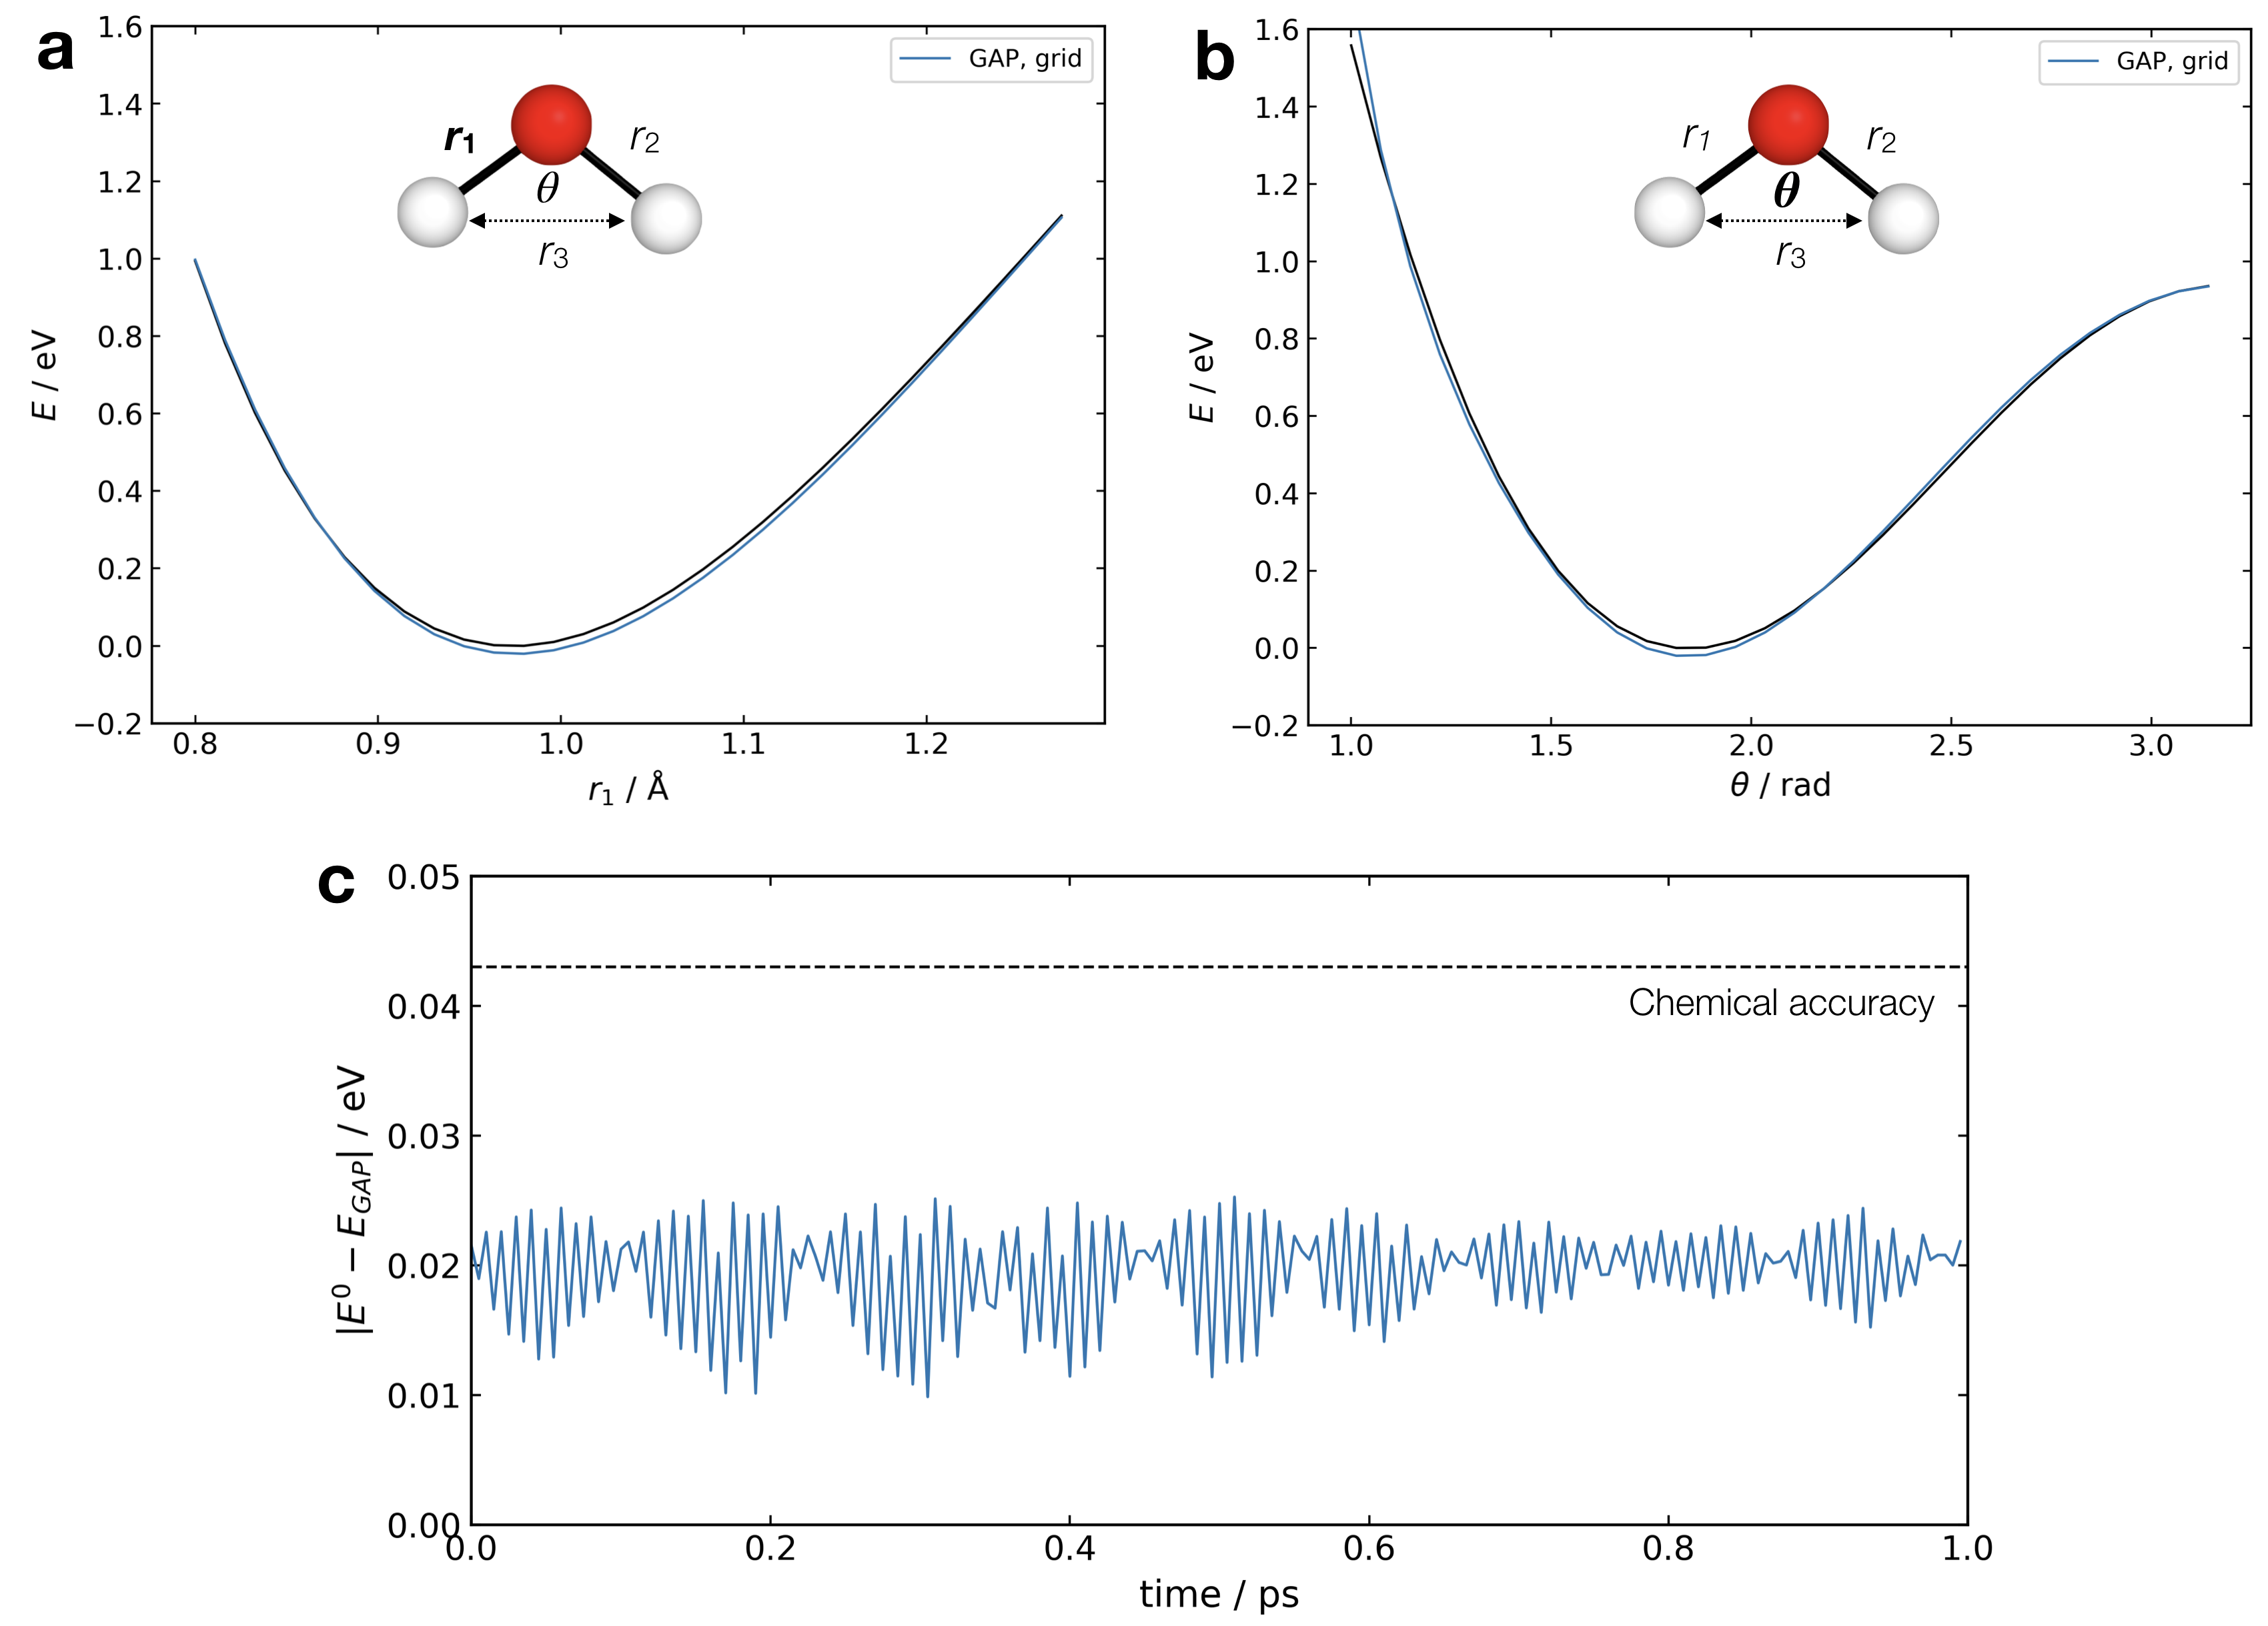
\includegraphics[width=\textwidth]{6/gap/figs_si/fig9}
	\vspace{0.2cm}
	\hrule
	\caption{Unrelaxed potential energy surfaces for the O-H stretch (a) and HOH bend (b) and (c) error in gas phase monomer dynamics generated by GAPs trained on 65 data points in a grid over $r_1, r_2 \in [0.8, 1.5]$ \AA, $r_3  \in [1.0, 2.5]$ \AA including the minimum at the DFTB(3ob parameters) level of theory. Two-body and three body GAP trained with 3.0 \AA$\;$ cut-offs.}
	\label{fig::ml_si_9}
\end{figure}



\begin{figure}[h!]
	\vspace{0.4cm}
	\centering
	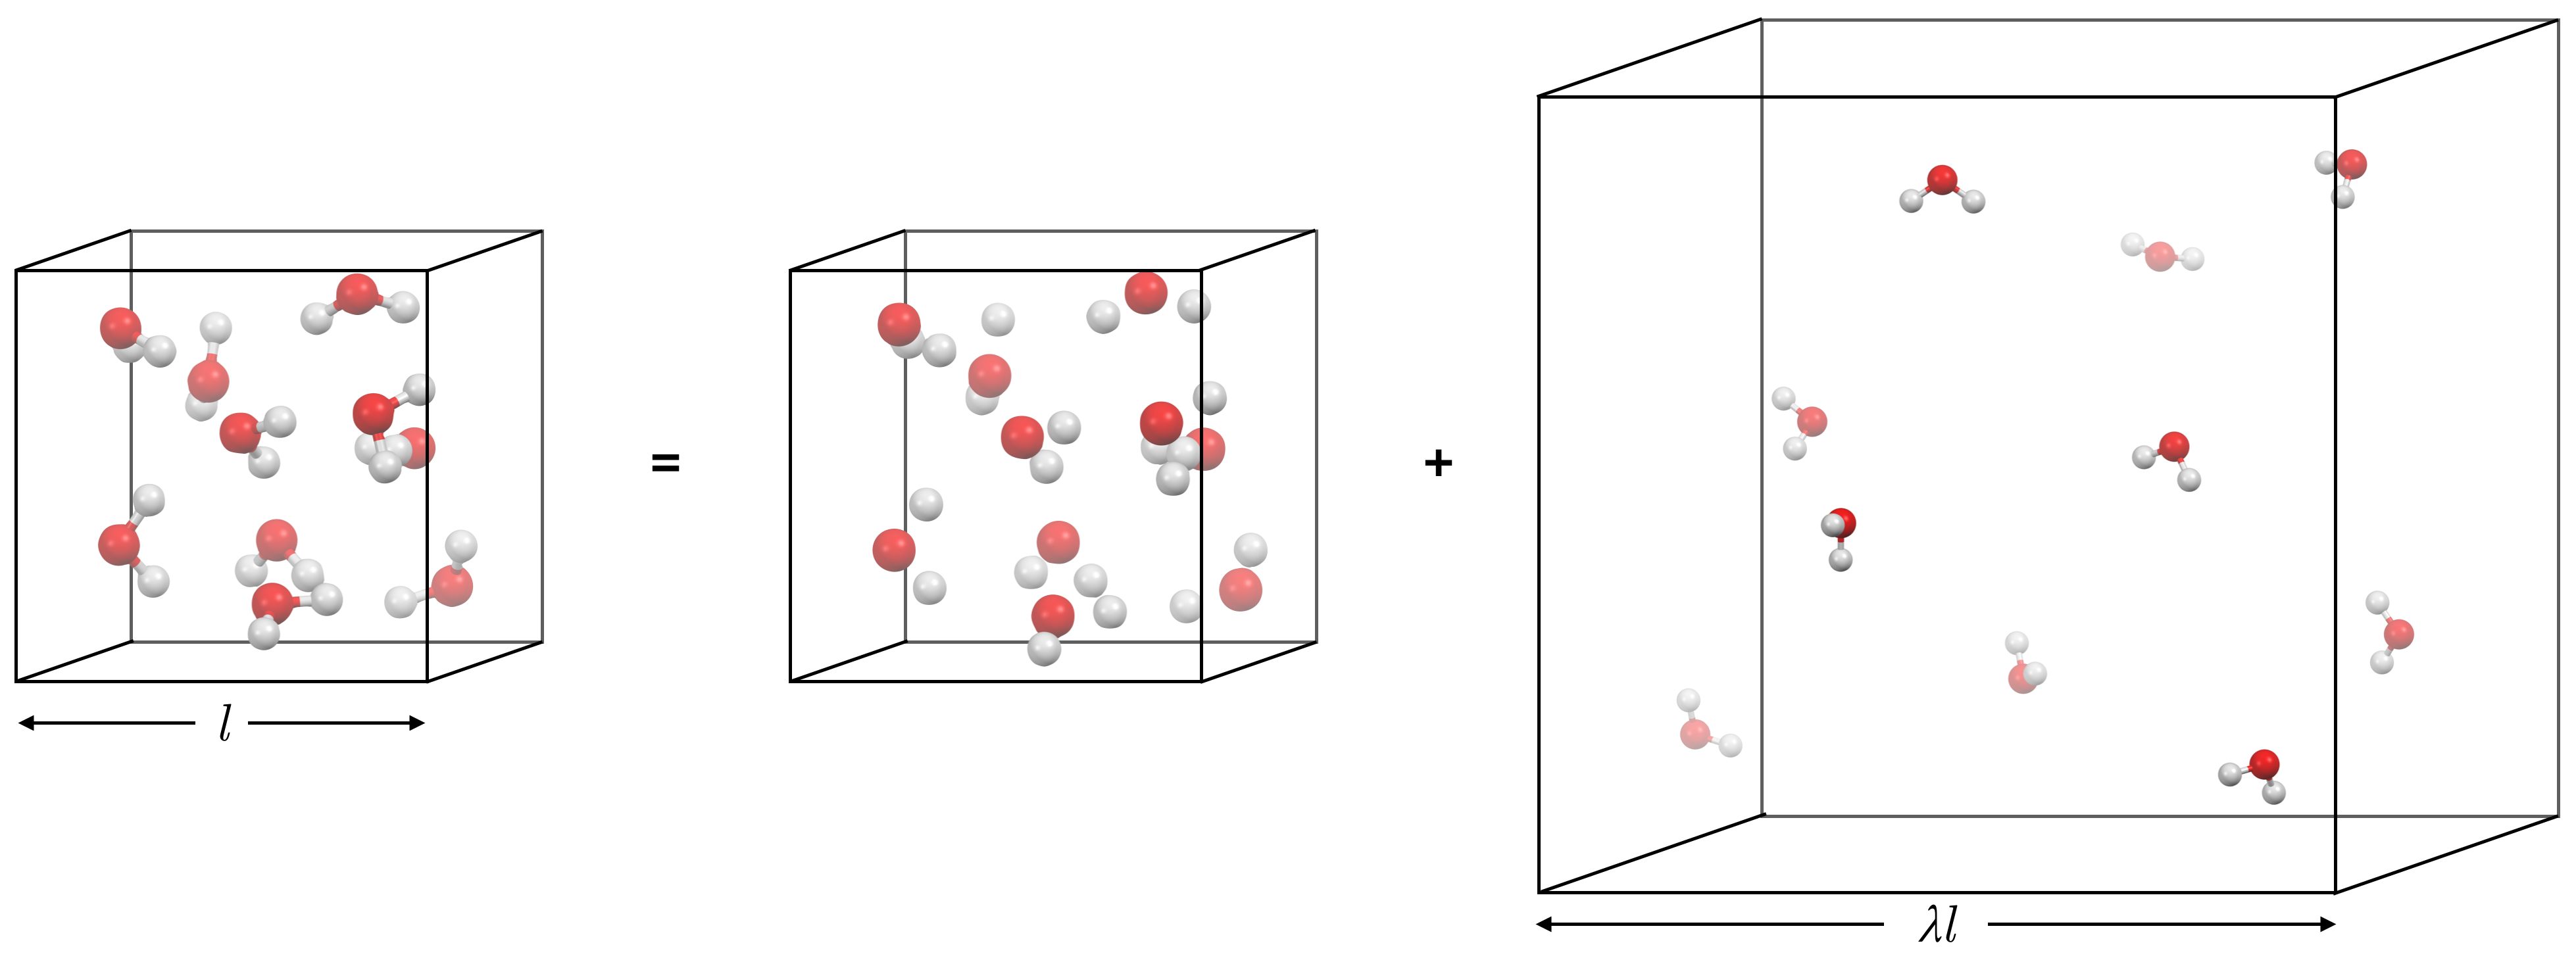
\includegraphics[width=\textwidth]{6/gap/figs_si/fig10}
	\vspace{0.2cm}
	\hrule
	\caption{Schematic representation of an intra+inter (II) energy evaluation using two GAPs. Total energy is a sum of the intermolecular interactions in a box, plus the intramolecular energy calculated by expanding the box by a factor $\lambda$, keeping the fractional centre of masses of each molecule fixed.}
	\label{fig::ml_si_10}
\end{figure}



\begin{figure}[h!]
	\vspace{0.4cm}
	\centering
	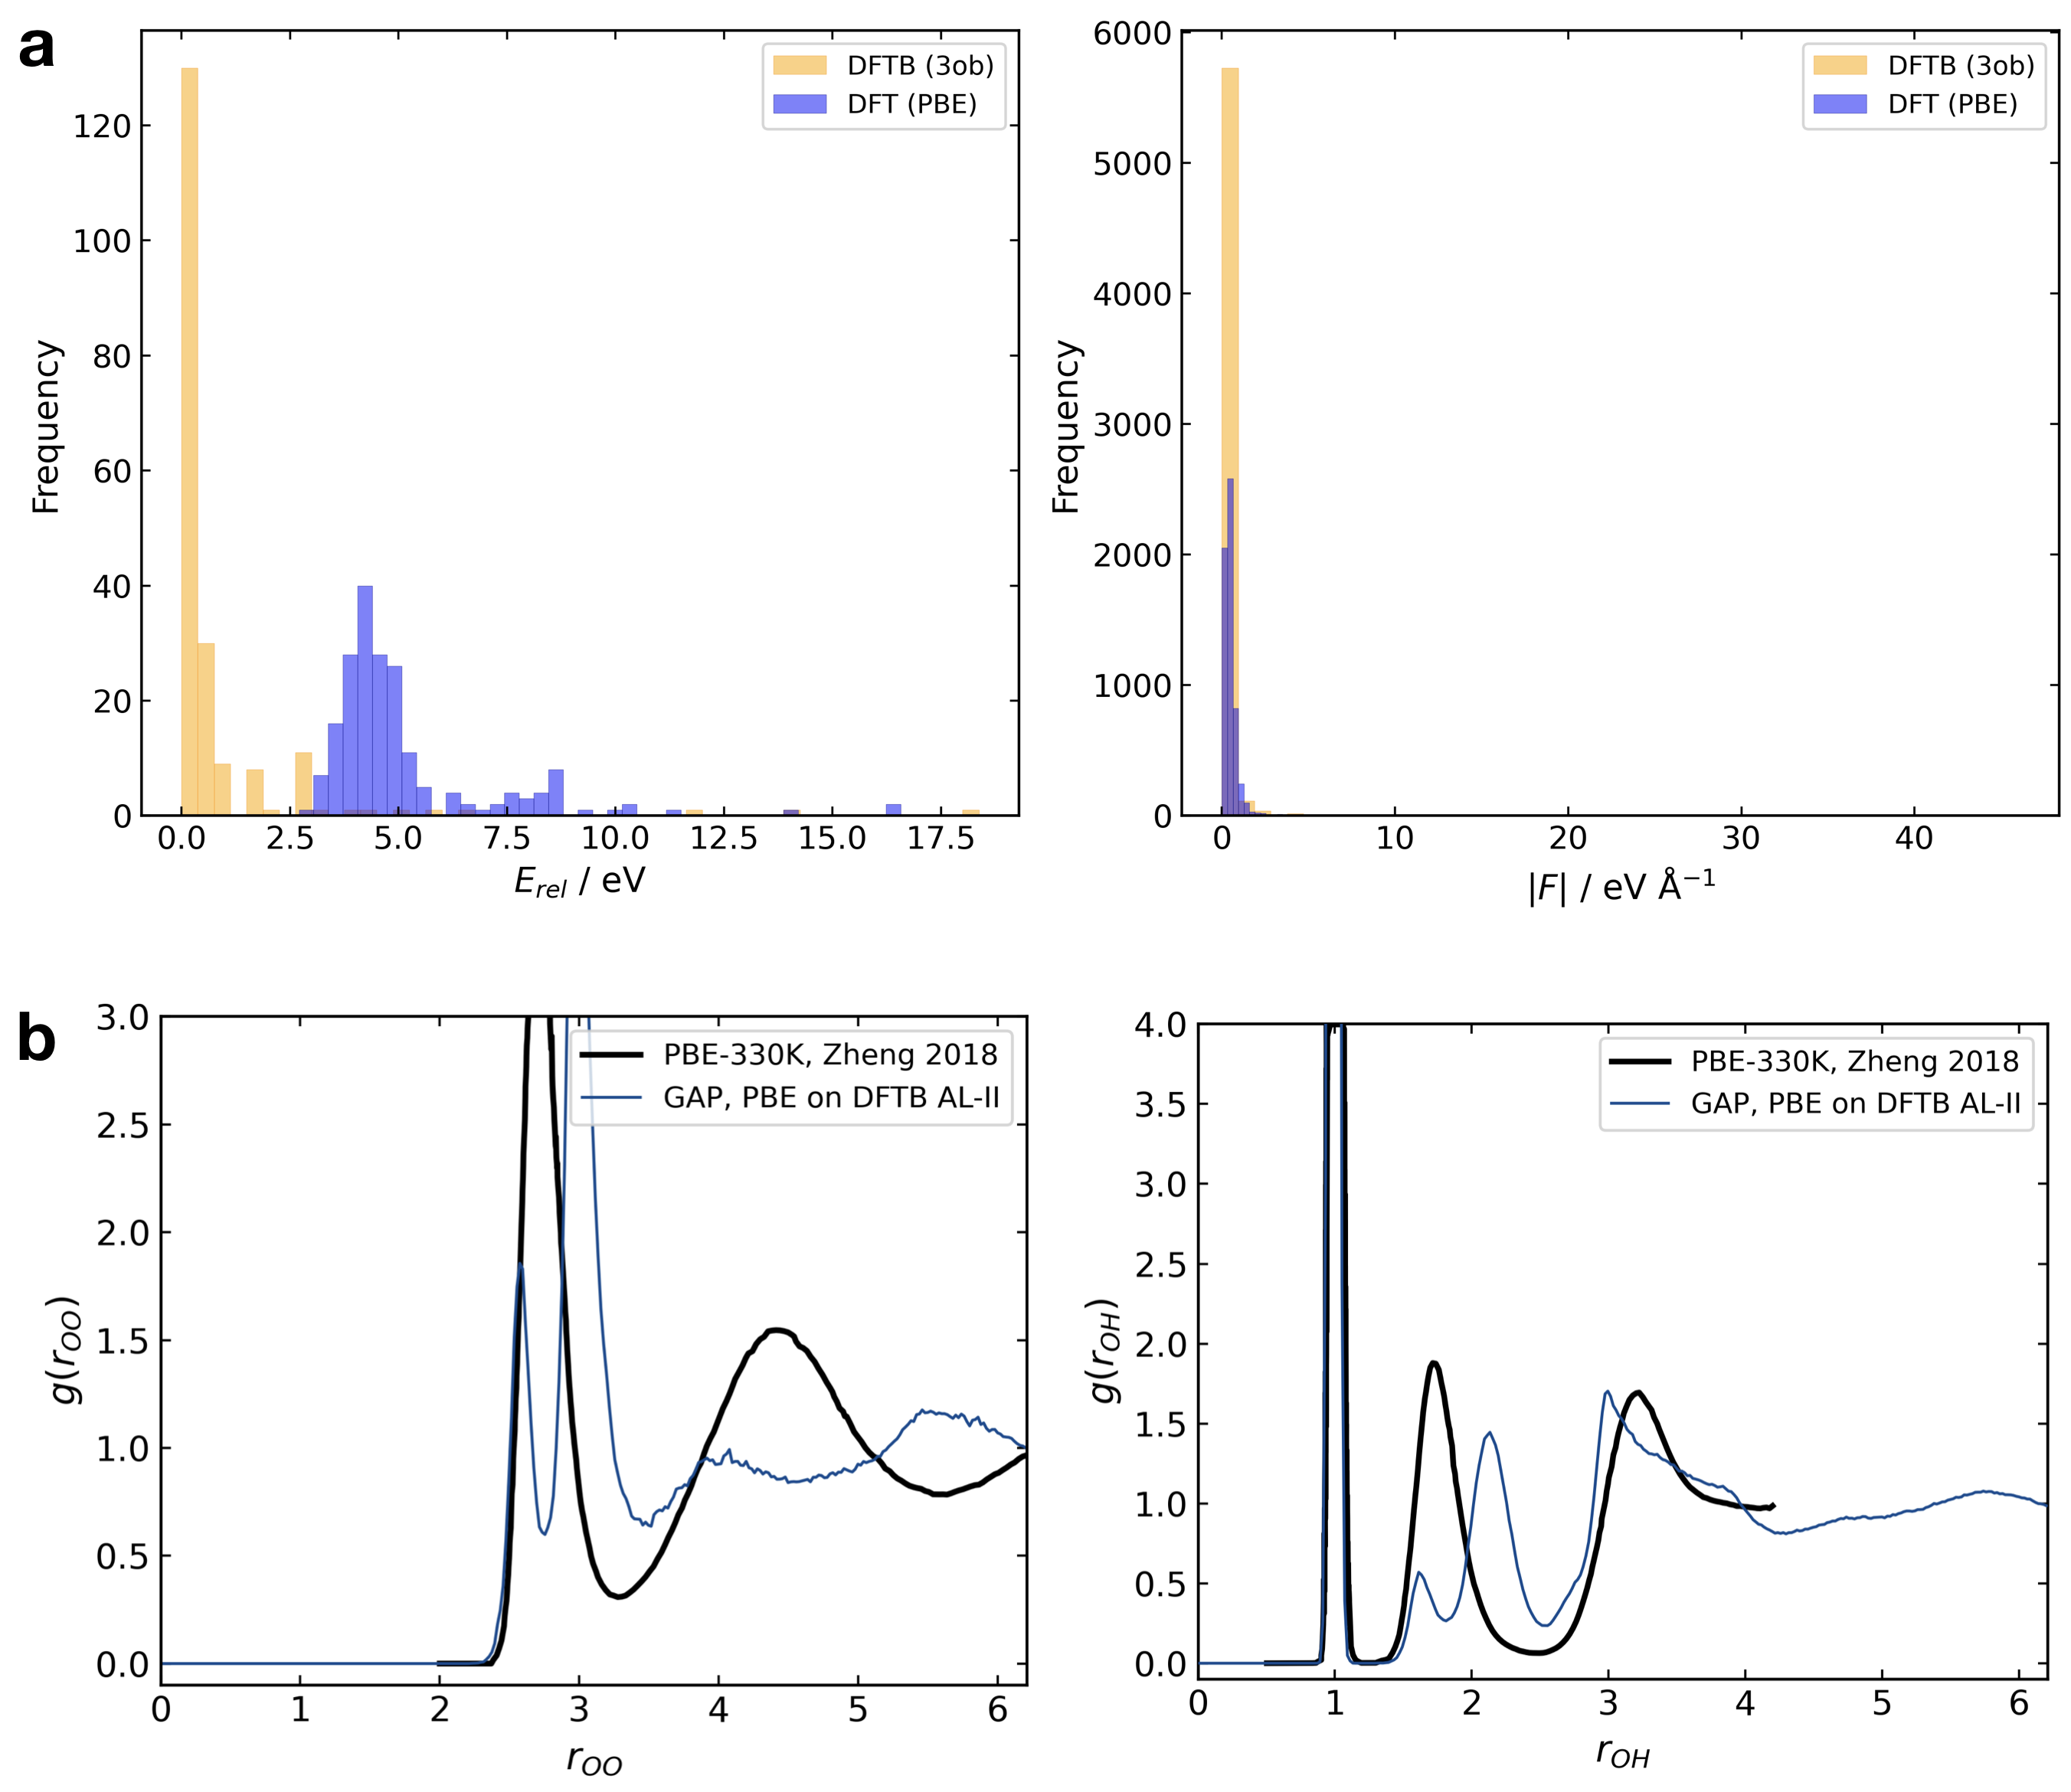
\includegraphics[width=\textwidth]{6/gap/figs_si/fig11}
	\vspace{0.2cm}
	\hrule
	\caption{Attempted DFT (PBE/400 eV) uplift of DFTB GAP with single point energy and force evaluations on a set of configurations used to train a stable inter GAP (AL-II, Figure \ref{fig::ml_1}). Intramolecular energy evaluated using a DFT GAP trained using active learning at 1600 K with a 2 eV maximum energy threshold. (a) Energy and force histograms, where the DFT configurations are referenced to the lowest energy located in an active learning cycle at the DFT level. (b) Pair radial distribution functions calculated from a 10 ps, 300 K MD simulations with the inter (+intra) GAP trained on the DFTB configurations, compared to a PBE reference from ref. \cite{Zheng2018}.}
	\label{fig::ml_si_11}
\end{figure}

\clearpage
\subsection{Other Solvents}

To demonstrate the transferability of the intra+inter active learning training method to other solvents presented here are learning curves in \taua for a selection of small, commonly used, organic solvents. The accuracy of the potential is quantified by the final error metric following the full active learning, and as a quick validation the radial distribution functions are shown for all pairs in each system. Given the much higher dimensionality of the intramolecular PES in all of the solvents a dense grid over all coordinates is not possible (e.g. $N_\text{atoms}$ = 6 in MeCN $= 8^{(3\times6) – 6} \sim 10^{11}$ points) and active learning needs to be employed for the intra surface. Employing active learning on the intramolecular modes of water requires both a high temperature, as to sample the curvature of the PES at regions often sampled at 300 K, and an energy threshold to prevent high energy configurations entering the fit (Figure \ref{fig::ml_si_13}).
Active learning at 1600 K then readily dissociates Cl radicals with a DFTB ground truth method.


\begin{figure}[h!]
	\vspace{0.4cm}
	\centering
	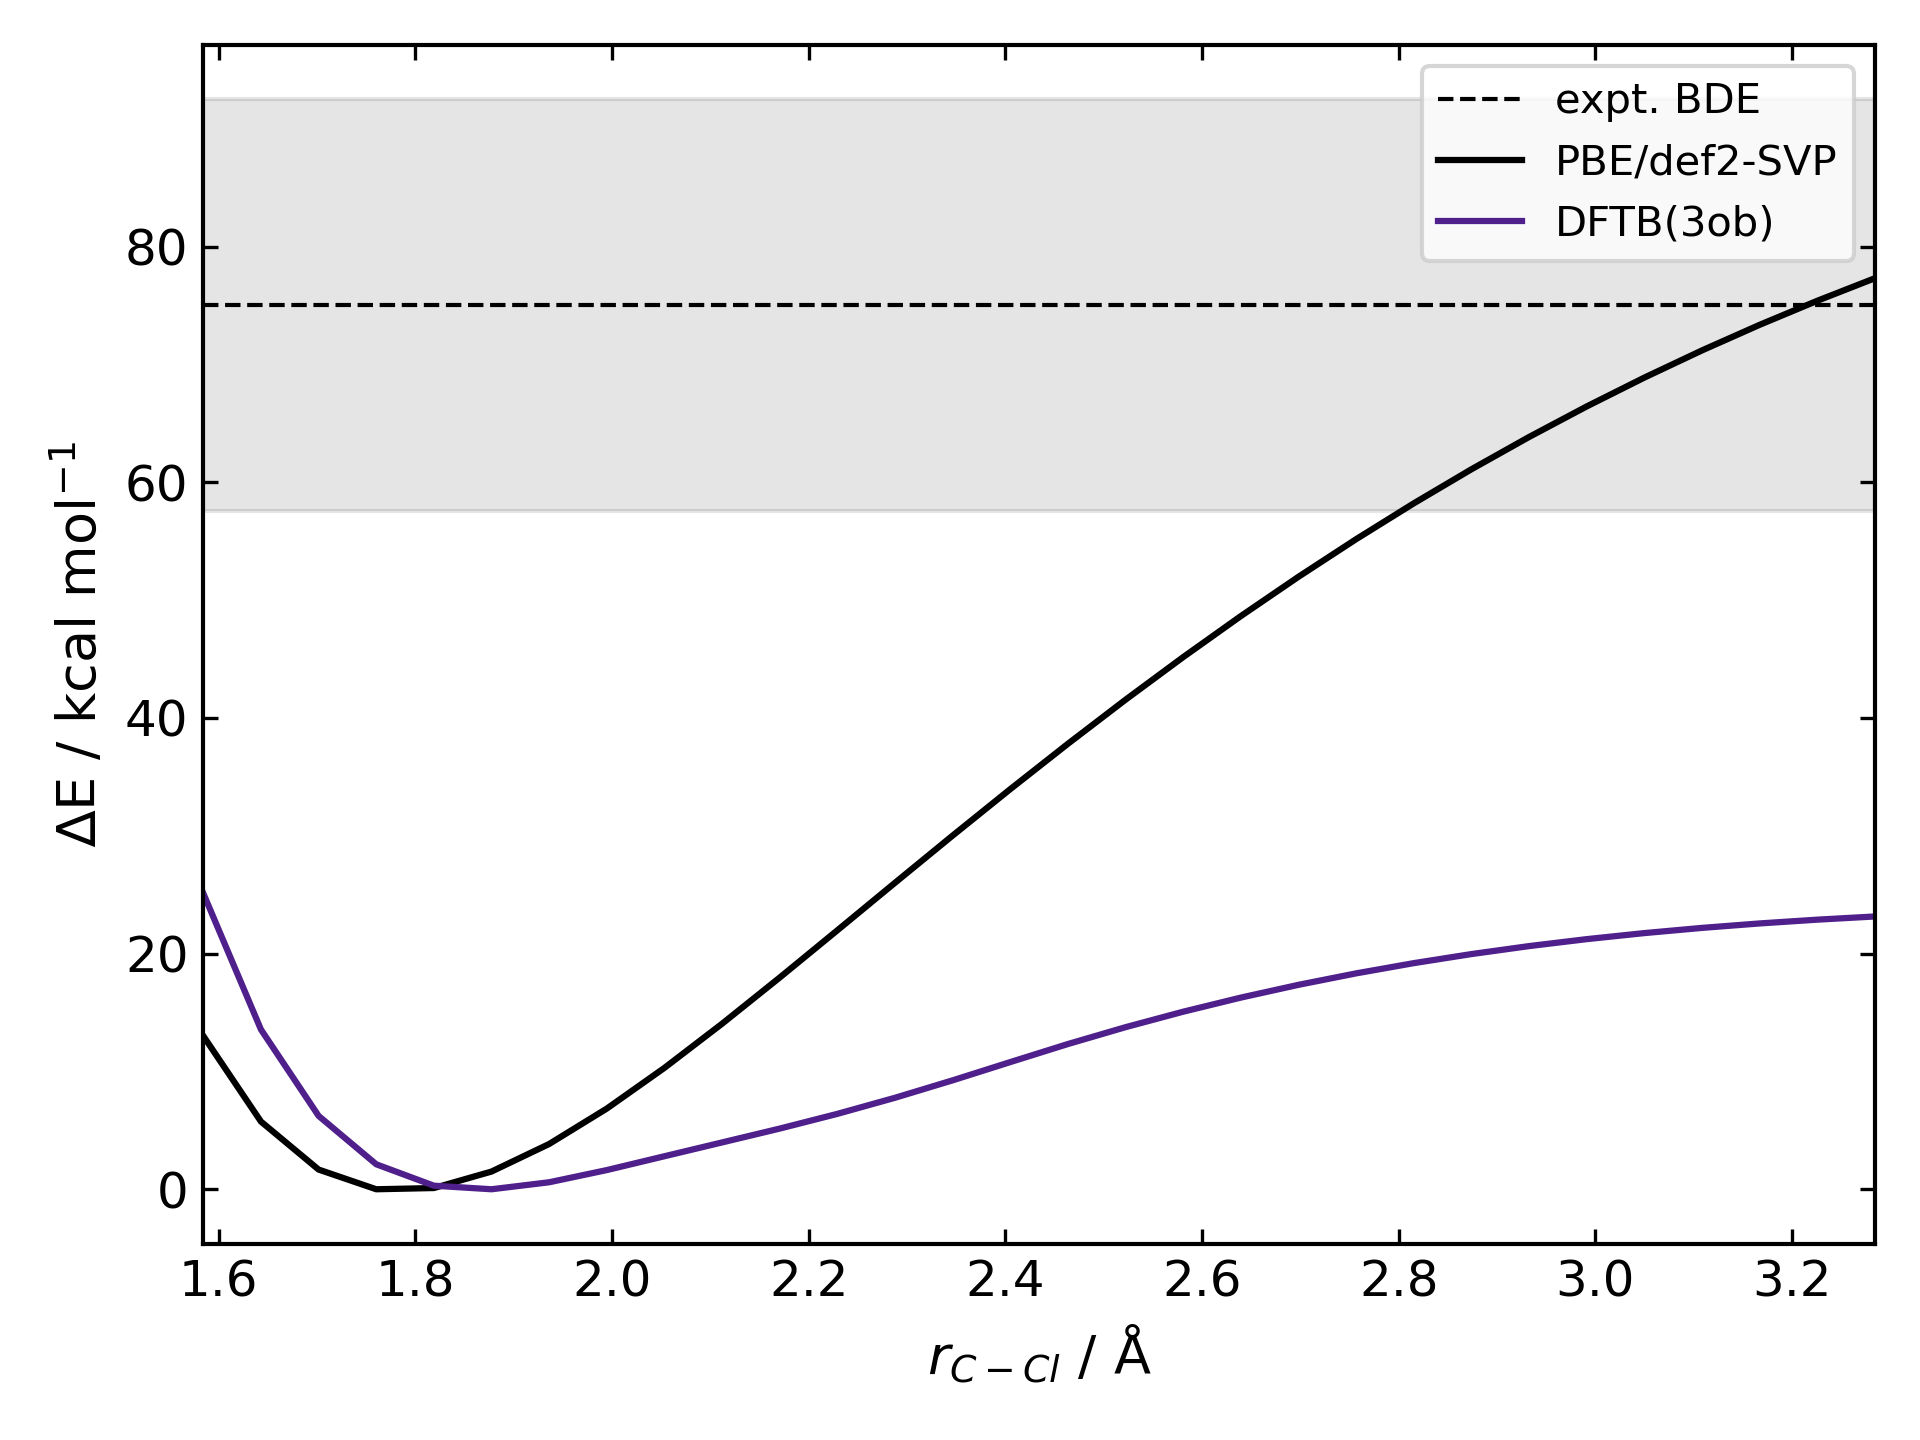
\includegraphics[width=10.5cm]{6/gap/figs_si/fig12}
	\vspace{0.2cm}
	\hrule
	\caption{Comparison between DFT (PBE/def2-SVP) and DFTB energies for the C–-Cl dissociation curve in CH${}_2$Cl${}_2$. Geometries from unrelaxed PES scan from the DFT geometry. Experimental data indicated with dash grey line from ref. \cite{Darwent1970}.}
	\label{fig::ml_si_12}
\end{figure}



\begin{figure}[h!]
	\vspace{0.4cm}
	\centering
	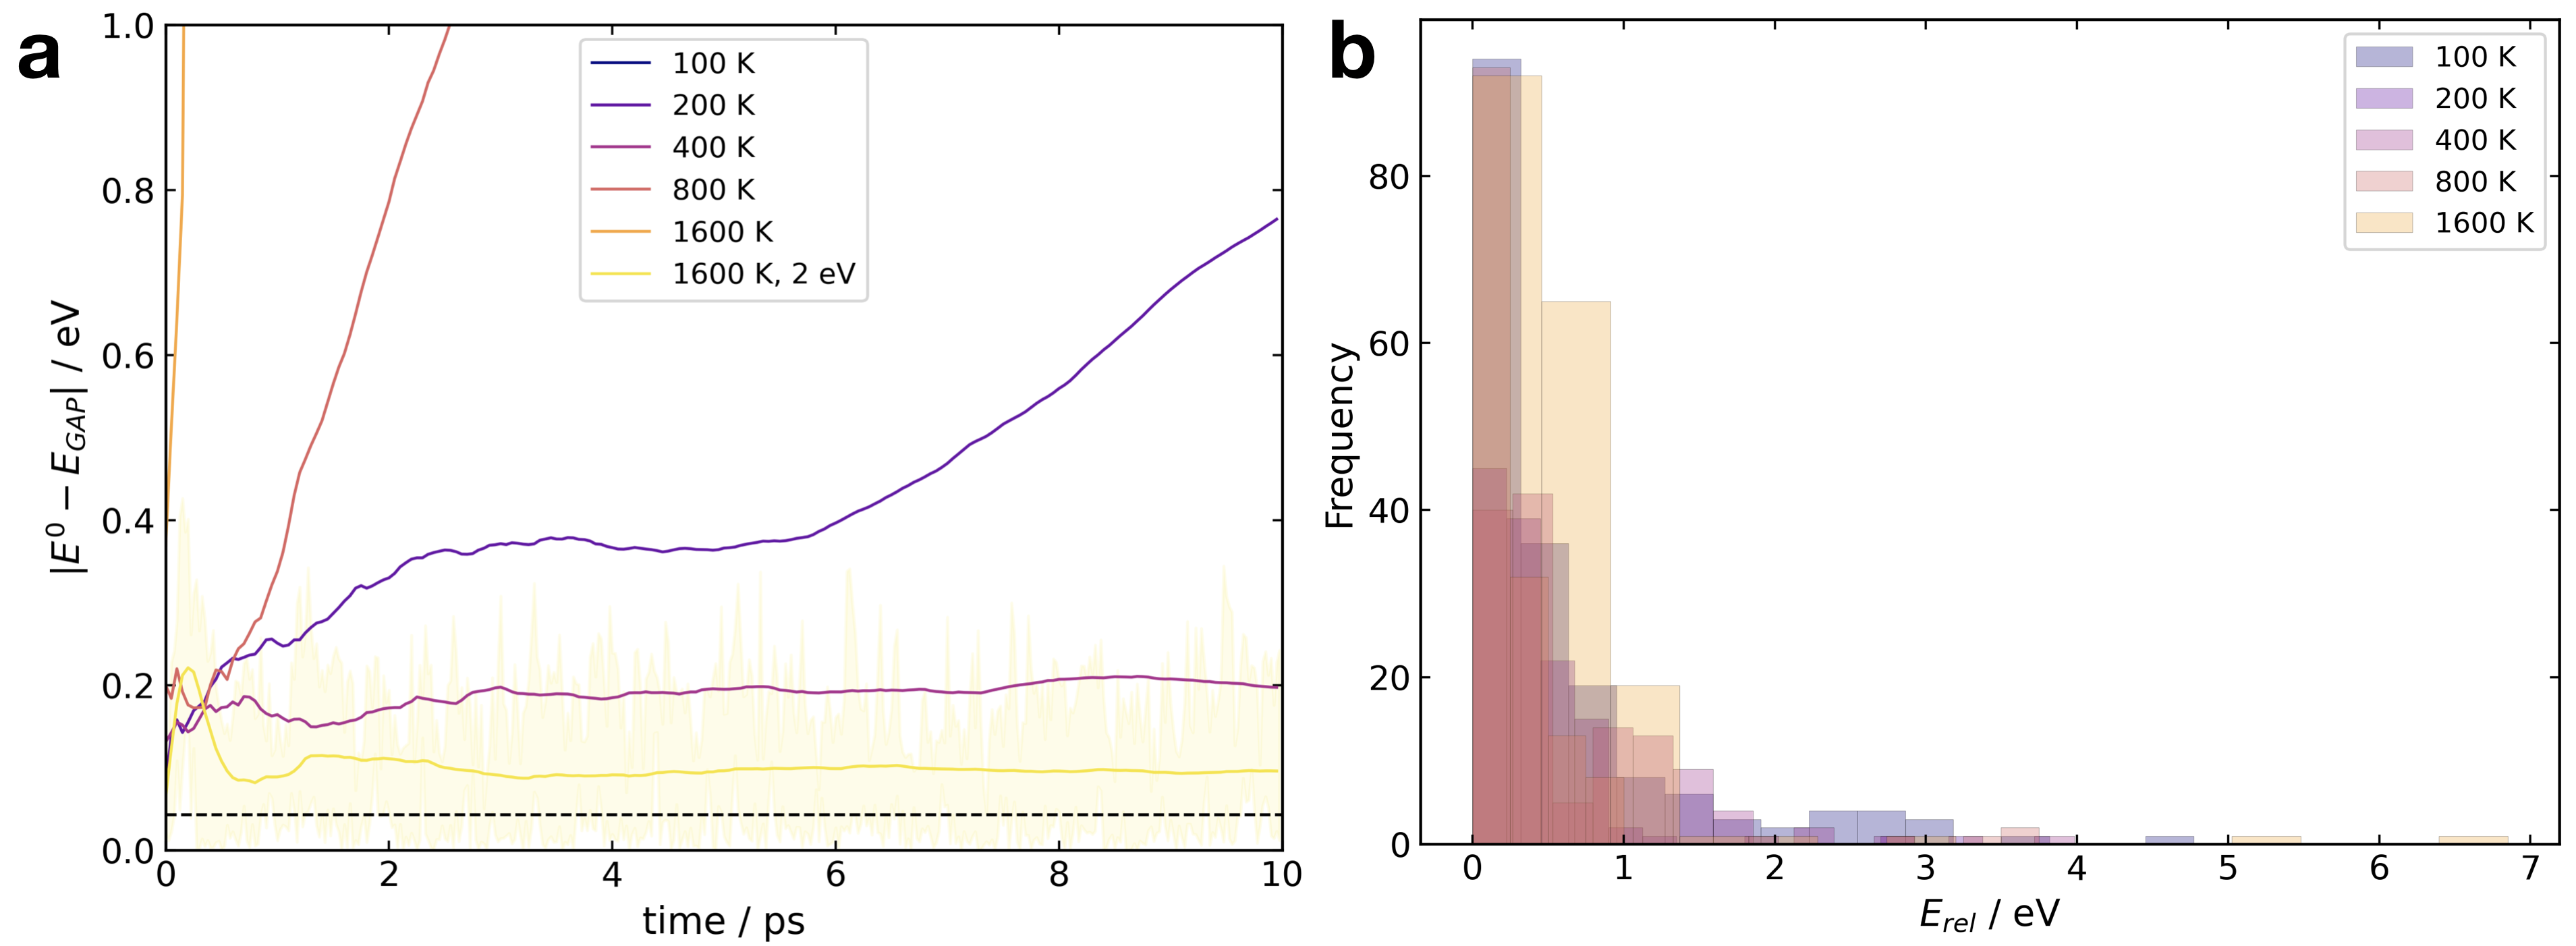
\includegraphics[width=\textwidth]{6/gap/figs_si/fig13}
	\vspace{0.2cm}
	\hrule
	\caption{Absolute errors between GAP and the ground truth DFTB on GAP-MD trajectories propagated at 300 K of a water box. Intramolecular GAP(2b+3b) trained using active learning using intermediate GAP-MD at the quoted temperature. 1600 K, 2 eV also specifies an energy cut-off on GAP training data. Intermolecular GAP trained as Figure \ref{fig::ml_1} (AL-I+I). Error ranges are generally not shown for clarity. Initial random configurations to start the active training loop are identical for each training run.}
	\label{fig::ml_si_13}
\end{figure}



\begin{figure}[h!]
	\vspace{0.4cm}
	\centering
	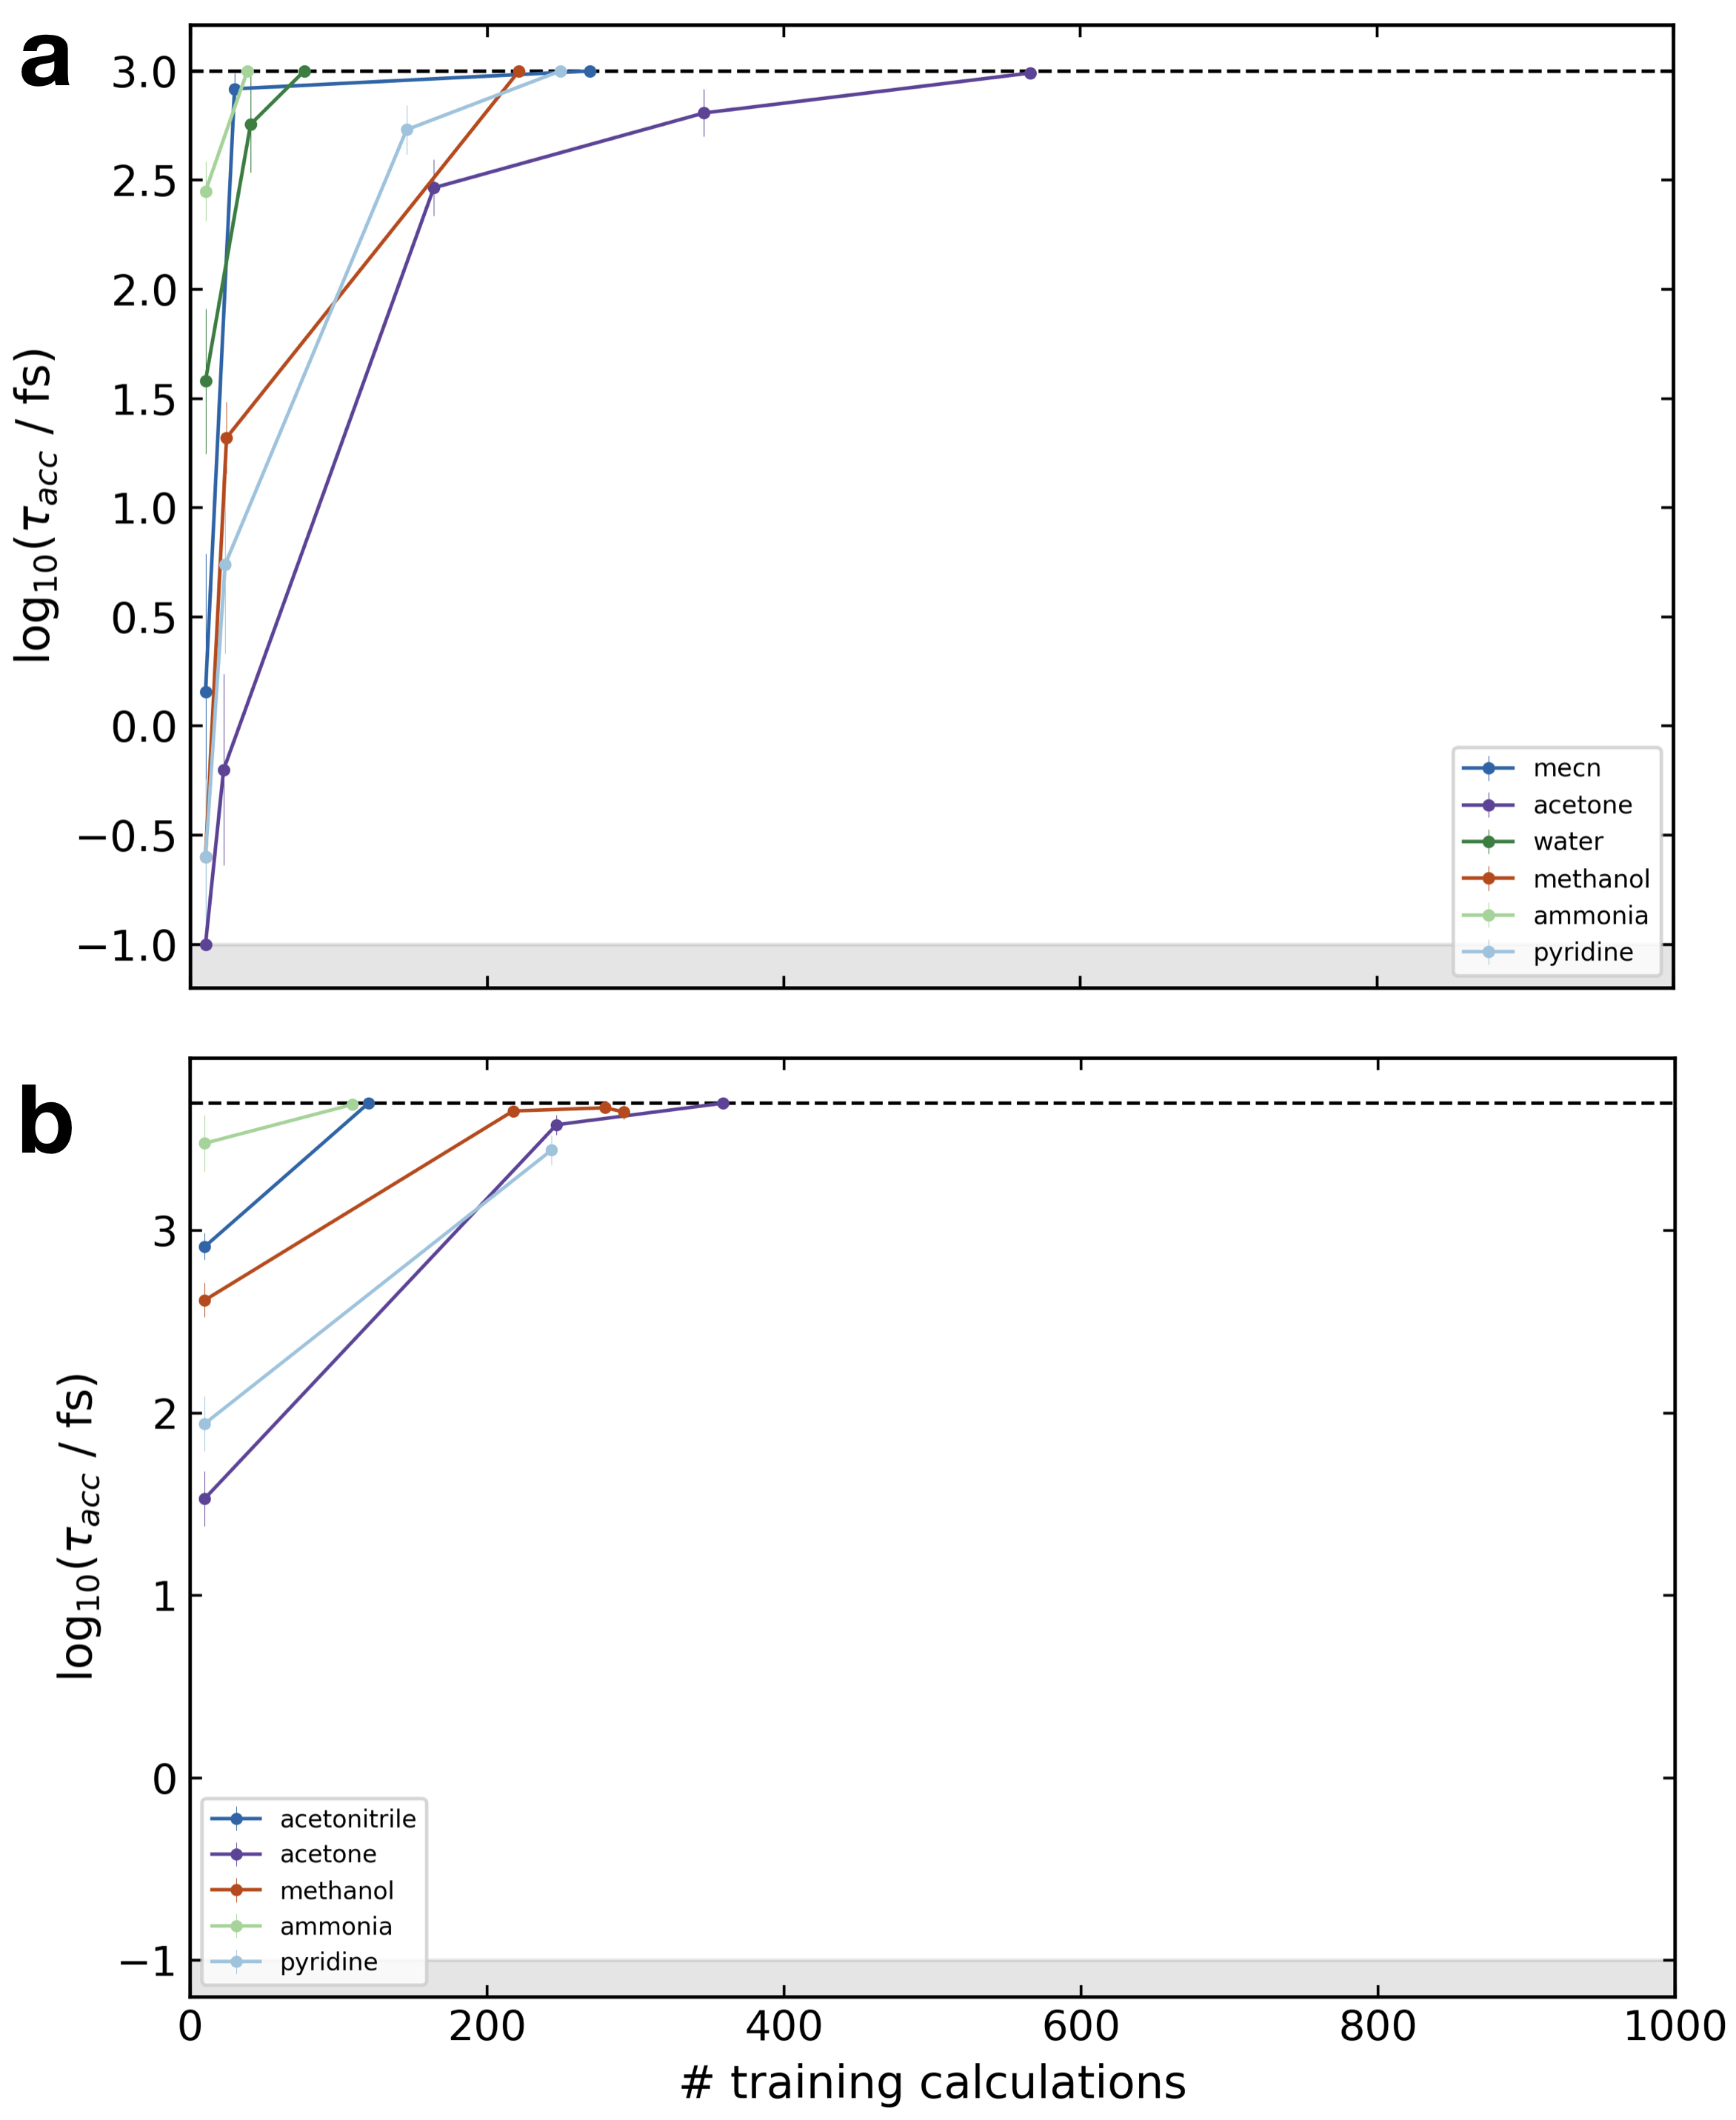
\includegraphics[width=10cm]{6/gap/figs_si/fig14}
	\vspace{0.2cm}
	\hrule
	\caption{Learning curves (a) intra- and (b)intermolecular components in different molecular solvents. Parameters for each system shown in full Supporting Information. 1600 K for all intramolecular active learning and 300 K for the intermolecular equivalent from 10 initial random normal displacements of all atoms ($\sigma$ = 0.05 \AA, $\mu$ = 0 \AA). Maximum \taua shown as dashed lines and $\min(\tau_\text{acc})$ = 0.1 fs for plotting. Error bars plotted as the standard error in the mean from 5 independent repeats. Active learning halted if no configurations have error above the threshold.}
	\label{fig::ml_si_14}
\end{figure}


\begin{figure}[h!]
	\vspace{0.4cm}
	\centering
    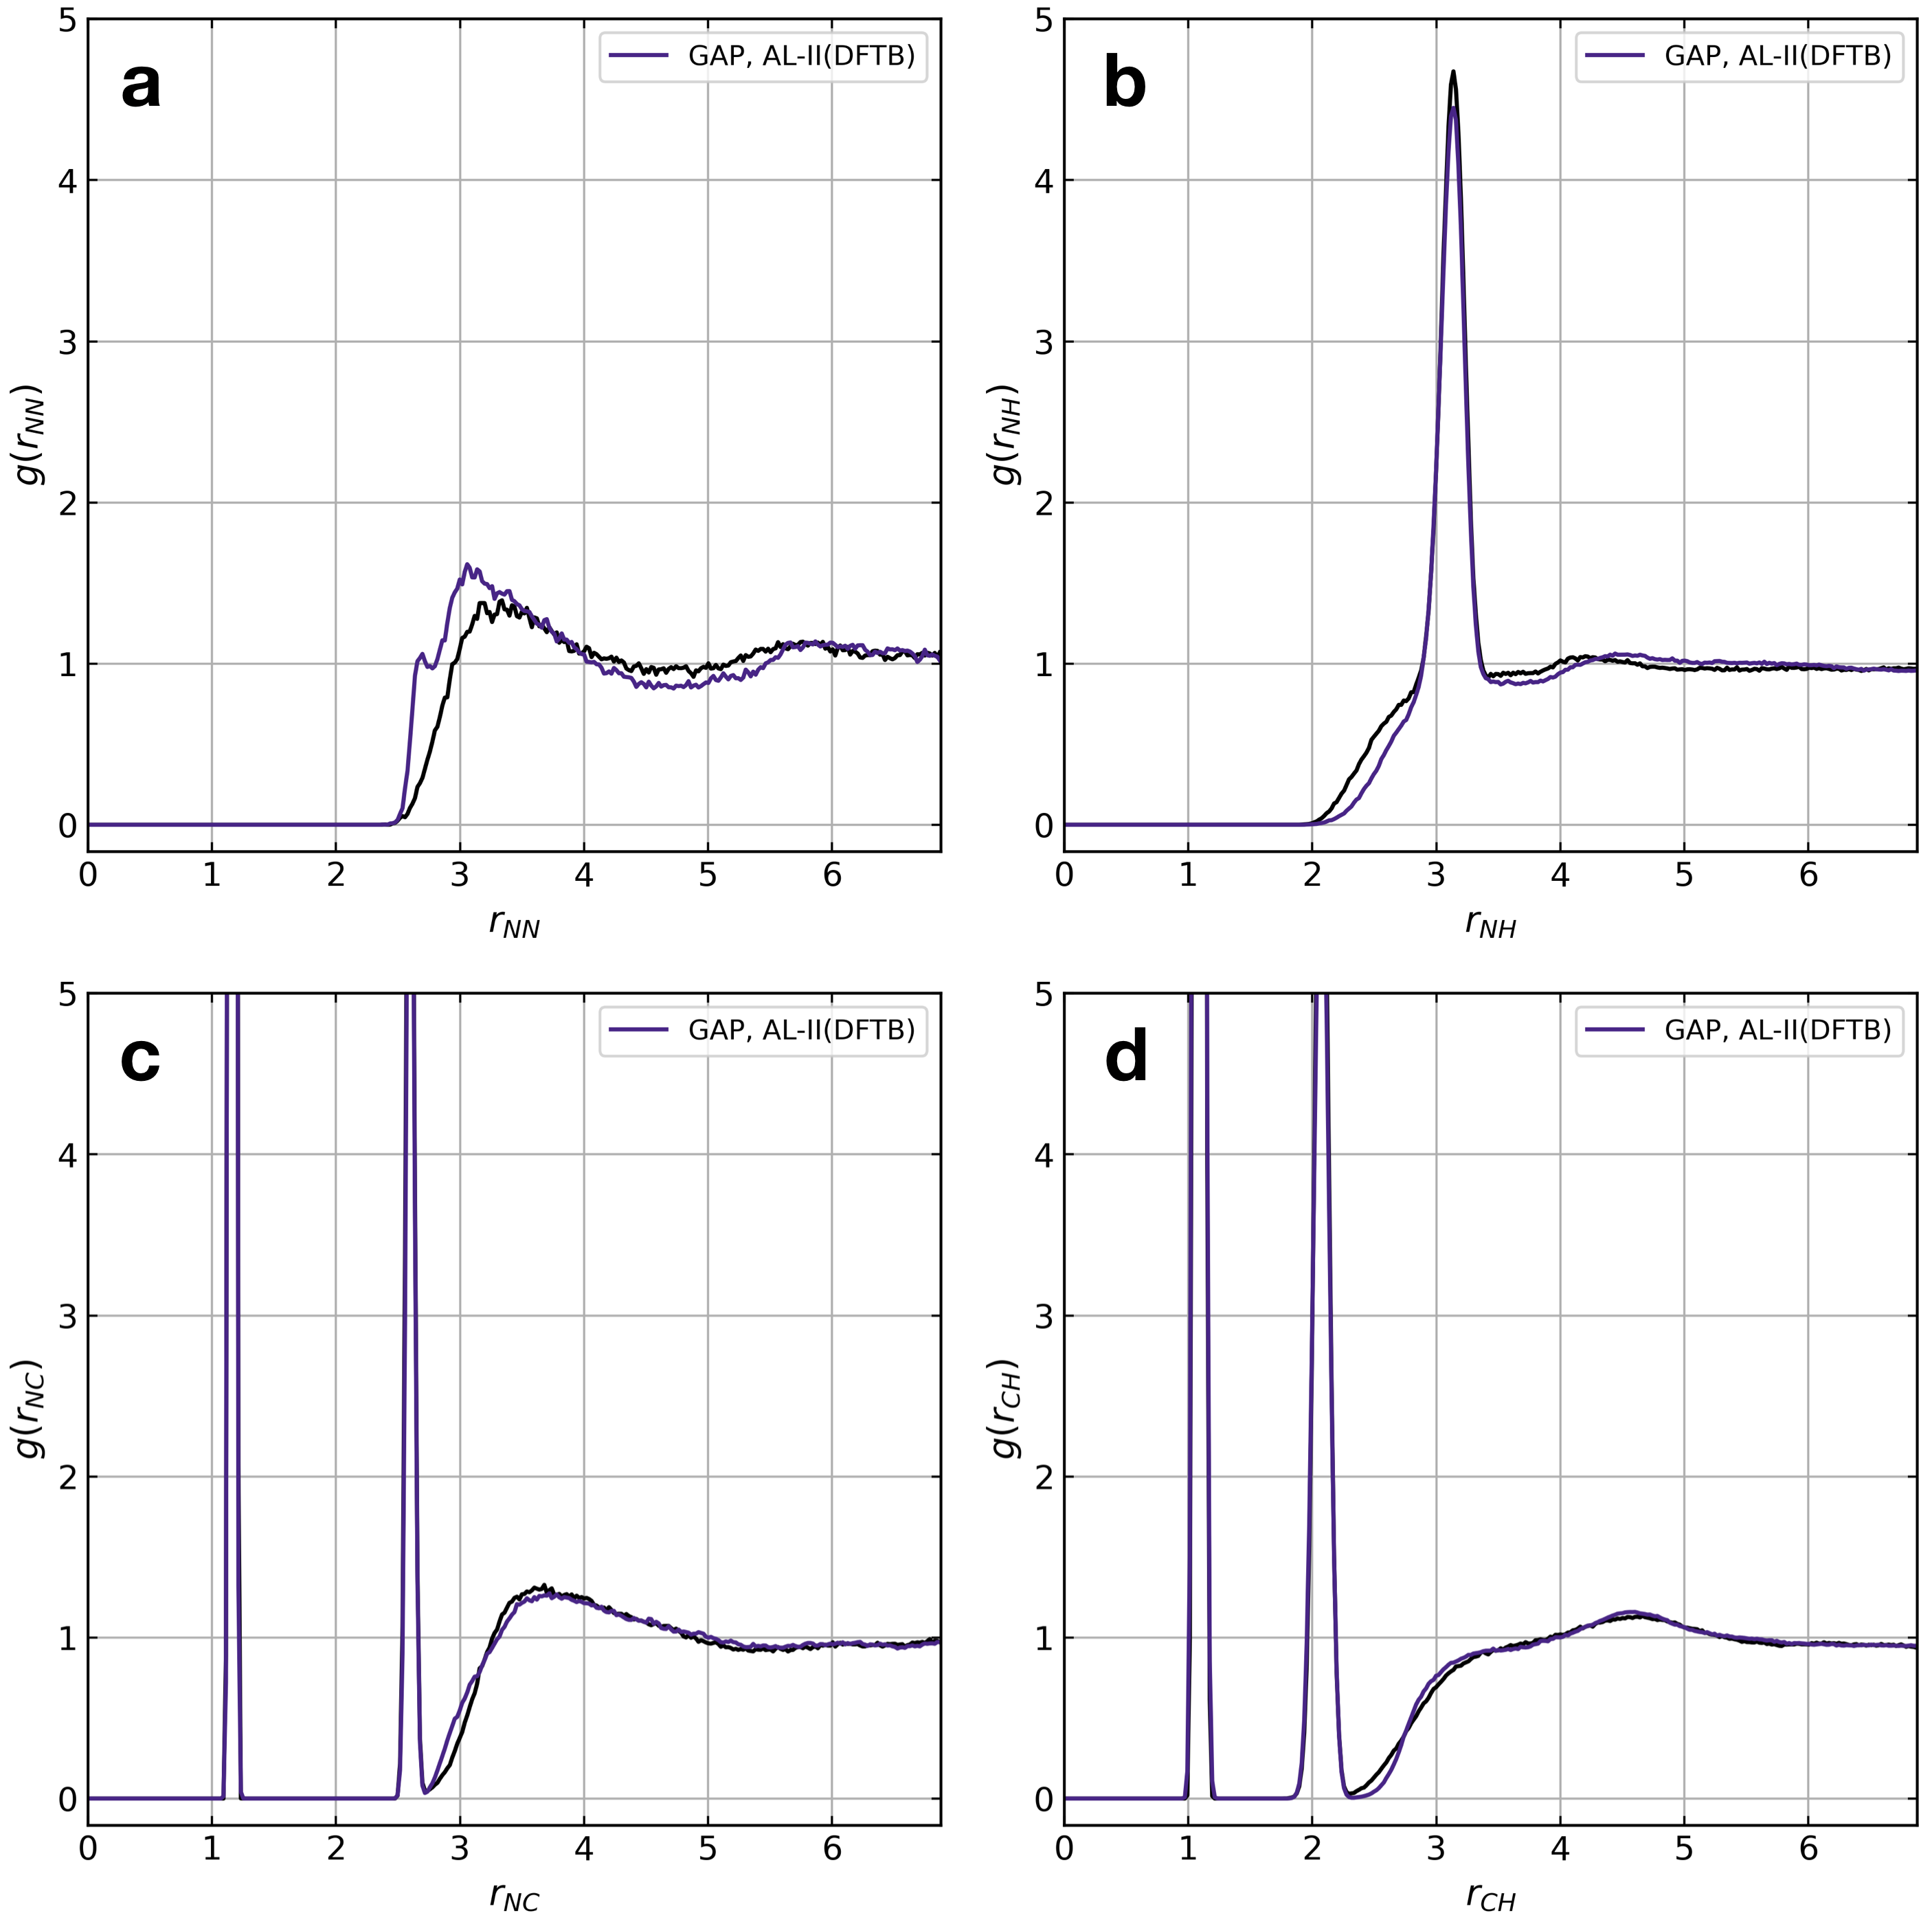
\includegraphics[width=14cm]{6/gap/figs_si/fig15}
	\vspace{0.2cm}
	\hrule
	\caption{Radial distributions functions for acetonitrile generated using GAPs (purple) trained with active learning on inter and intramolecular degrees of freedom (as Figure \ref{fig::ml_si_14}) ground truth DFTB(3ob) level (black). Dynamics run for 30 ps at 300 K in a 13.8 \AA length box with a time-step of 0.5 fs.}
	\label{fig::ml_si_15}
\end{figure}

\clearpage 
\subsection{Reactions}


\begin{figure}[h!]
	\vspace{0.4cm}
	\centering
	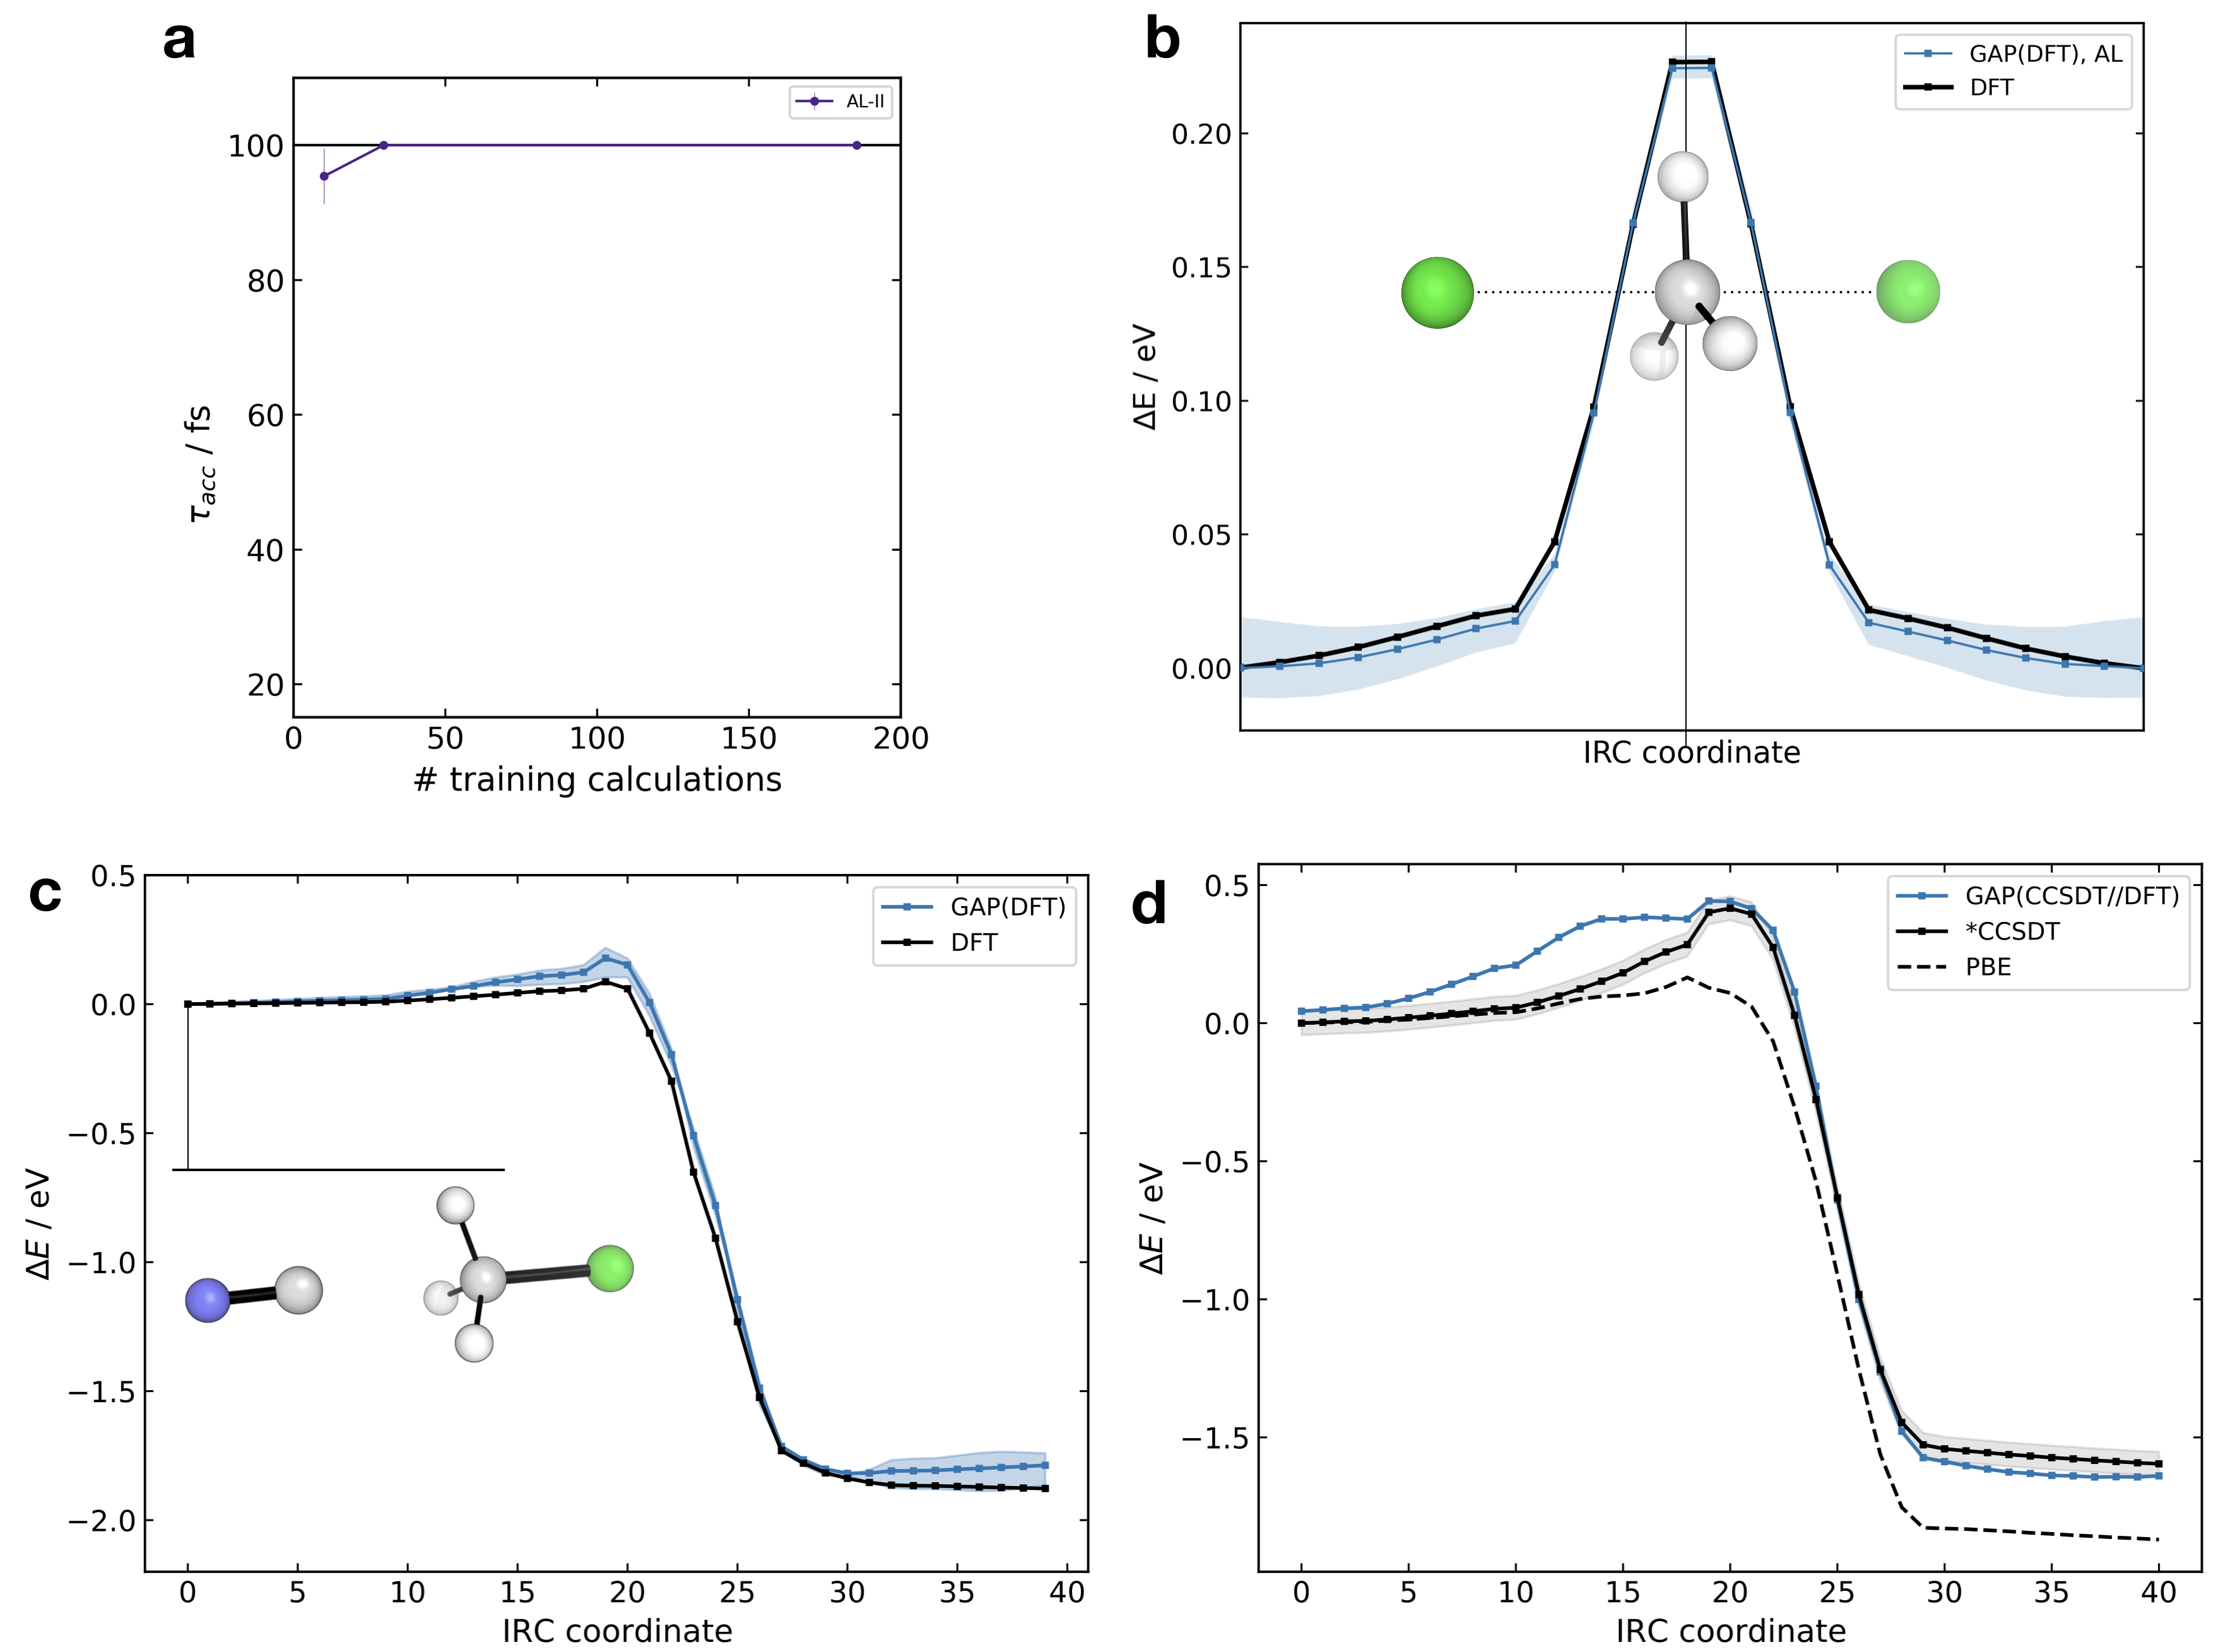
\includegraphics[width=15cm]{6/gap/figs_si/fig16}
	\vspace{0.2cm}
	\hrule
	\caption{(a) Learning curve for TS originated dynamics in the gas phase for Cl${}^{-}$ + CH${}_{3}$Cl $\rightarrow$ Cl${}^{-}$ + CH${}_{3}$Cl. Number of ground truth evaluations does not include those used to find the initial transition state. SOAP descriptors with $r_c$ = 3.5 \AA on C and Cl. TS optimisation and energy/force evaluations performed with ORCA at the PBE/ma-def2-SVP level of theory. \taua calculated using a 2 fs time interval, 1 \kcalx error threshold, 10 \kcalx maximum total error to a maximum of \taua = 100 fs, as only short time dynamics are required from the TS. (b) IRC for Cl${}^{-}$ + CH${}_{3}$Cl $\rightarrow$ Cl${}^{-}$ + CH${}_{3}$Cl calculated in ORCA at the ground truth (PBE/ma-def2-SVP) and predicted with 5 trained GAPs. Average shown as the blue line and the range of predictions in blue. IRC configurations were not present in the training data. (c) As (b) for CN${}^{-}$ + CH${}_{3}$Cl $\rightarrow$ Cl${}^{-}$ + CH${}_{3}$CN but trained using uphill active learning i.e. without knowledge of the TS. 0.5 eV of energy was added to the breaking C–Cl bond and dynamics propagated for up to 500 fs at a temperature of 200 K. (d) Predicted IRC using the active-learnt GAP with configurations added from close to the minimum energy pathway with NEB relaxation (final geometry selected manually) using the GAP, energies and forces calculated, then re-predicted. Coupled cluster single point energies and numerical frequencies were then calculated on the 200 configurations and the IRC compared. *CCSD(T) $\equiv$ DLPNO-CCSD(T)/ma-def2-TZVPP) energy values on the MP2/ma-def2-TZVPP.}
	\label{fig::ml_si_16}
\end{figure}


\begin{figure}[h!]
	\vspace{0.4cm}
	\centering
	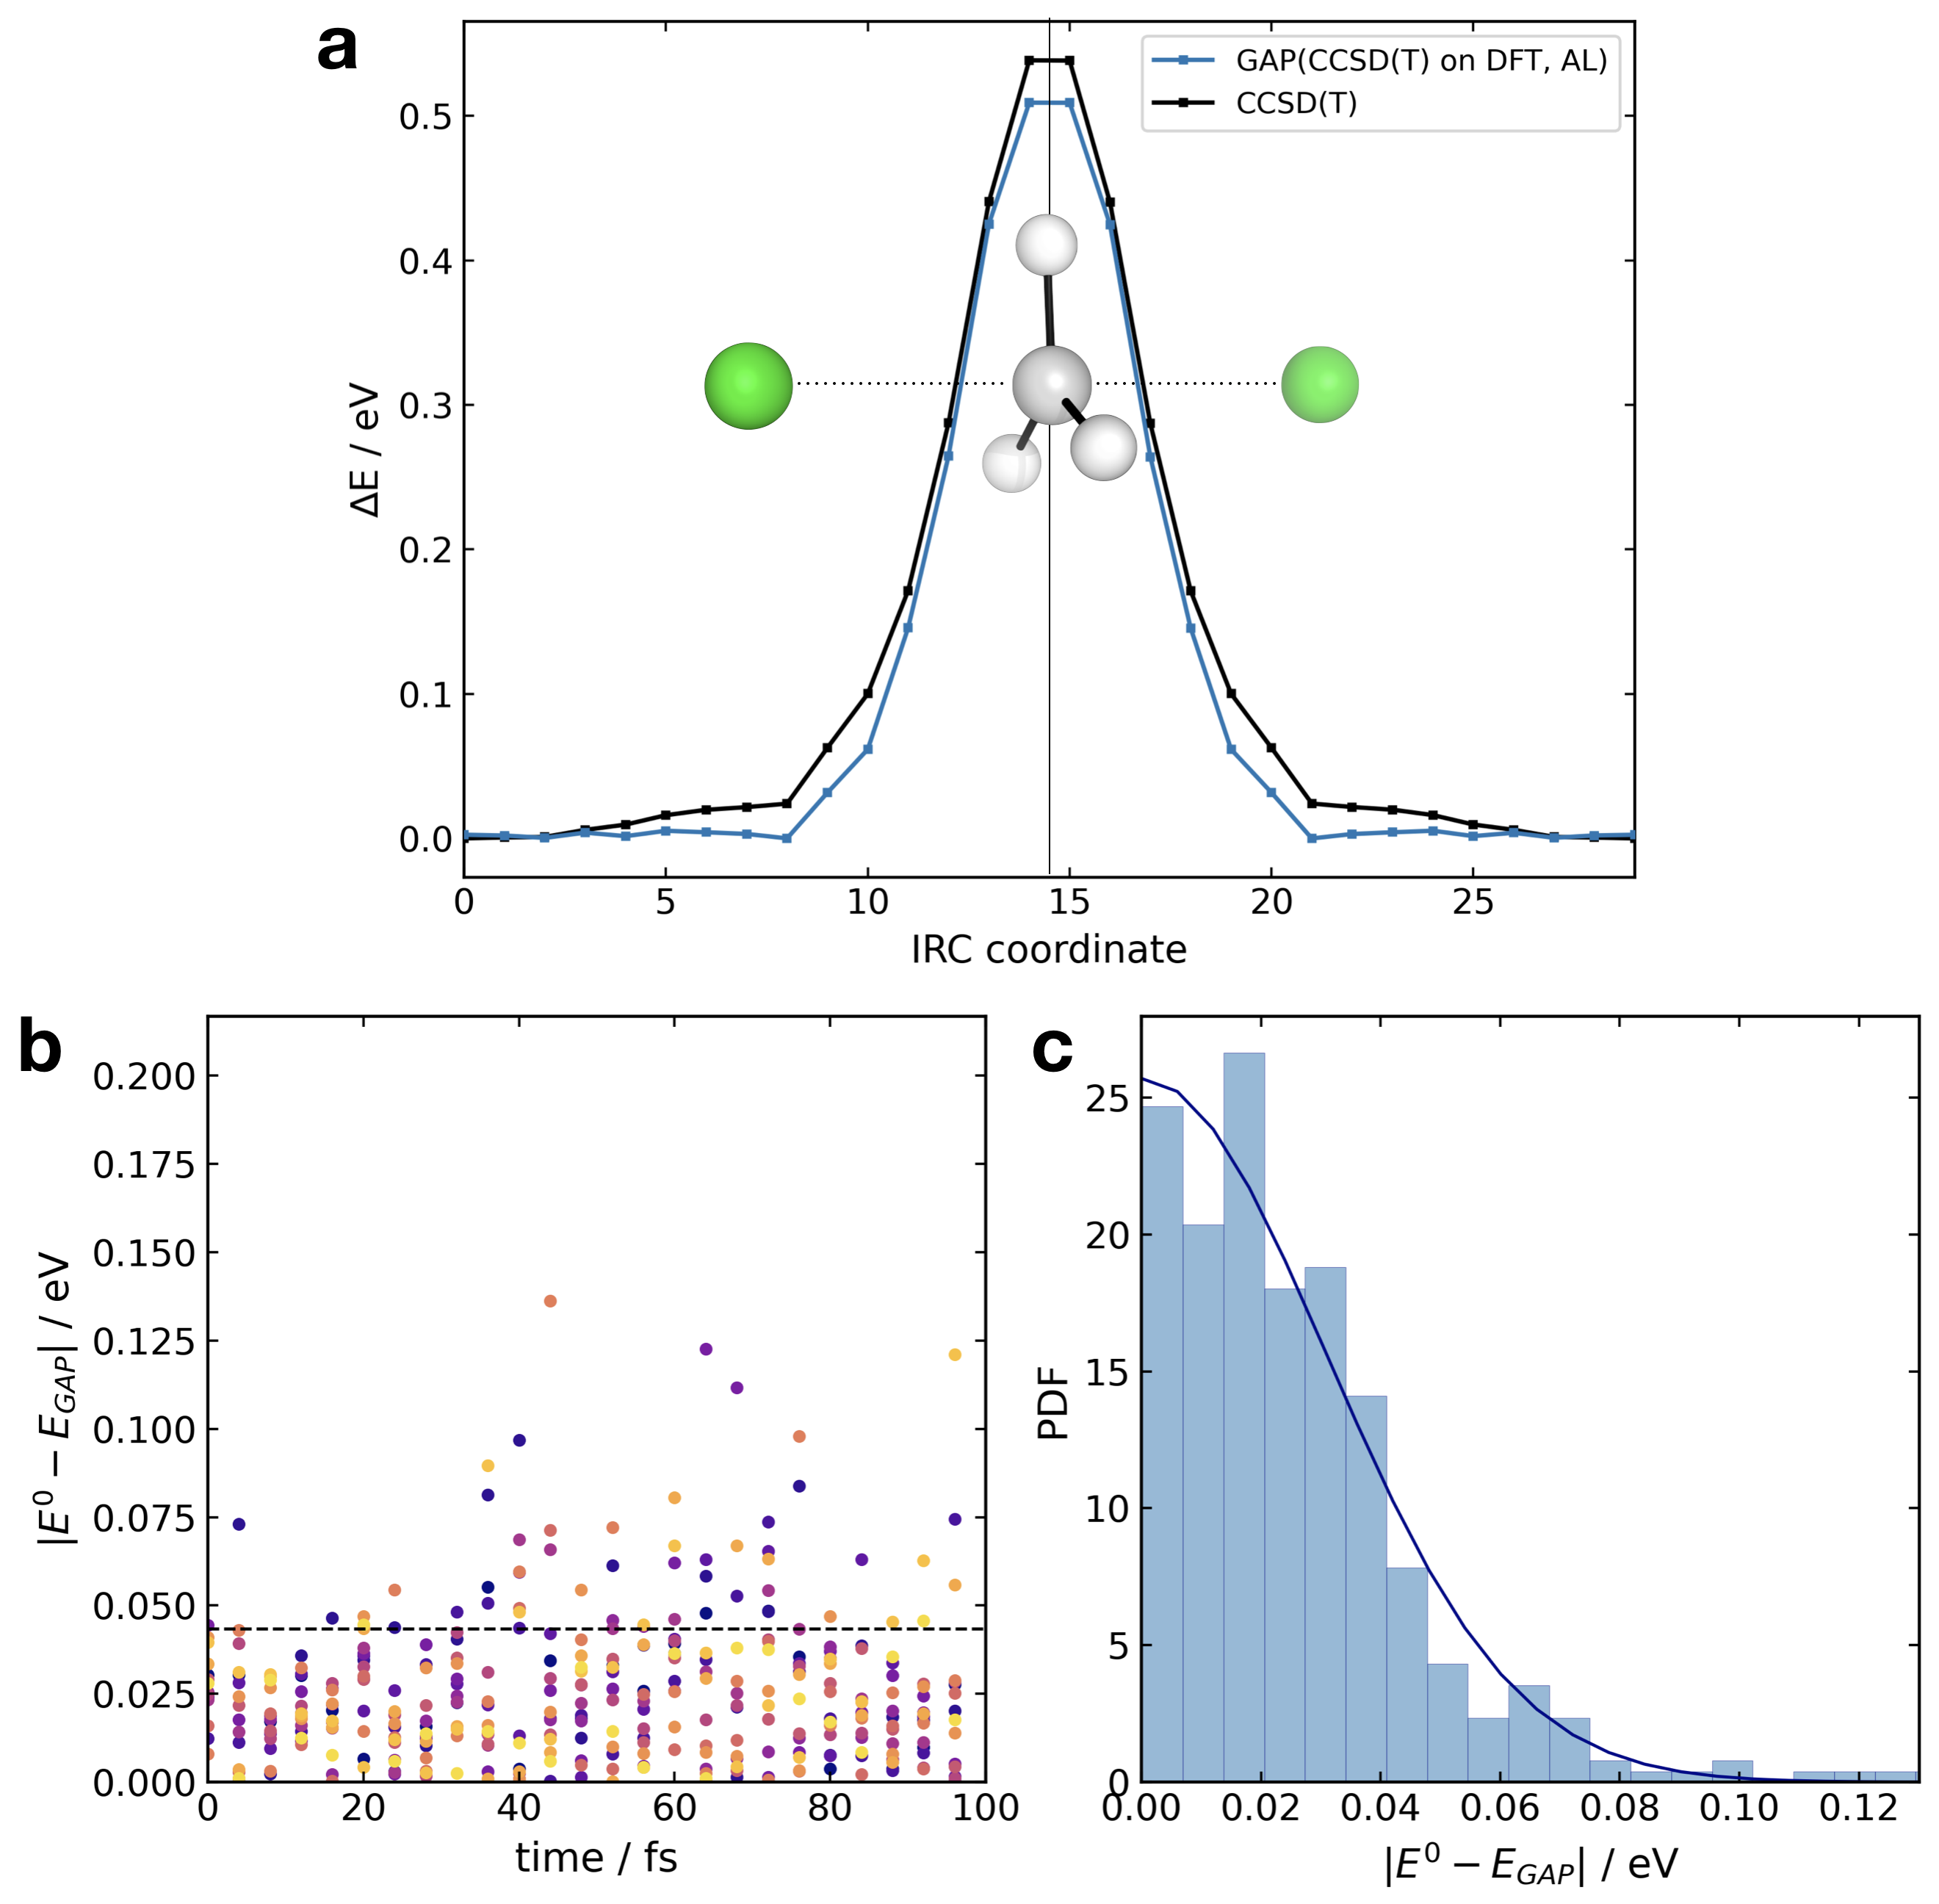
\includegraphics[width=0.8\textwidth]{6/gap/figs_si/fig17}
	\vspace{0.2cm}
	\hrule
	\caption{(a) Accuracy of a GAP trained on configurations generated from DFT (PBE/ma-def2-SVP) active learning (Figure \ref{fig::ml_si_16} for Cl${}^{-}$ + CH${}_{3}$Cl $\rightarrow$ Cl${}^{-}$ + CH${}_{3}$Cl from the TS. The energy profile is compared to the values obtained with an IRC calculation at the MP2/ma-def2-TZVPP level of theory from a MP2 optimised TS. CCSD(T)/ma-def2-TZVPP energy calculations on DFT configurations used numerical gradients over 55 configurations. (b/c) Error in dynamics calculated from 300 K MD simulations propagated with the trained GAP from the MP2 transition state. SOAP only descriptors on C and Cl with $r_c^\text{SOAP}$ = 3.5 \AA.}
	\label{fig::ml_si_17}
\end{figure}



\begin{figure}[h!]
	\vspace{0.4cm}
	\centering
	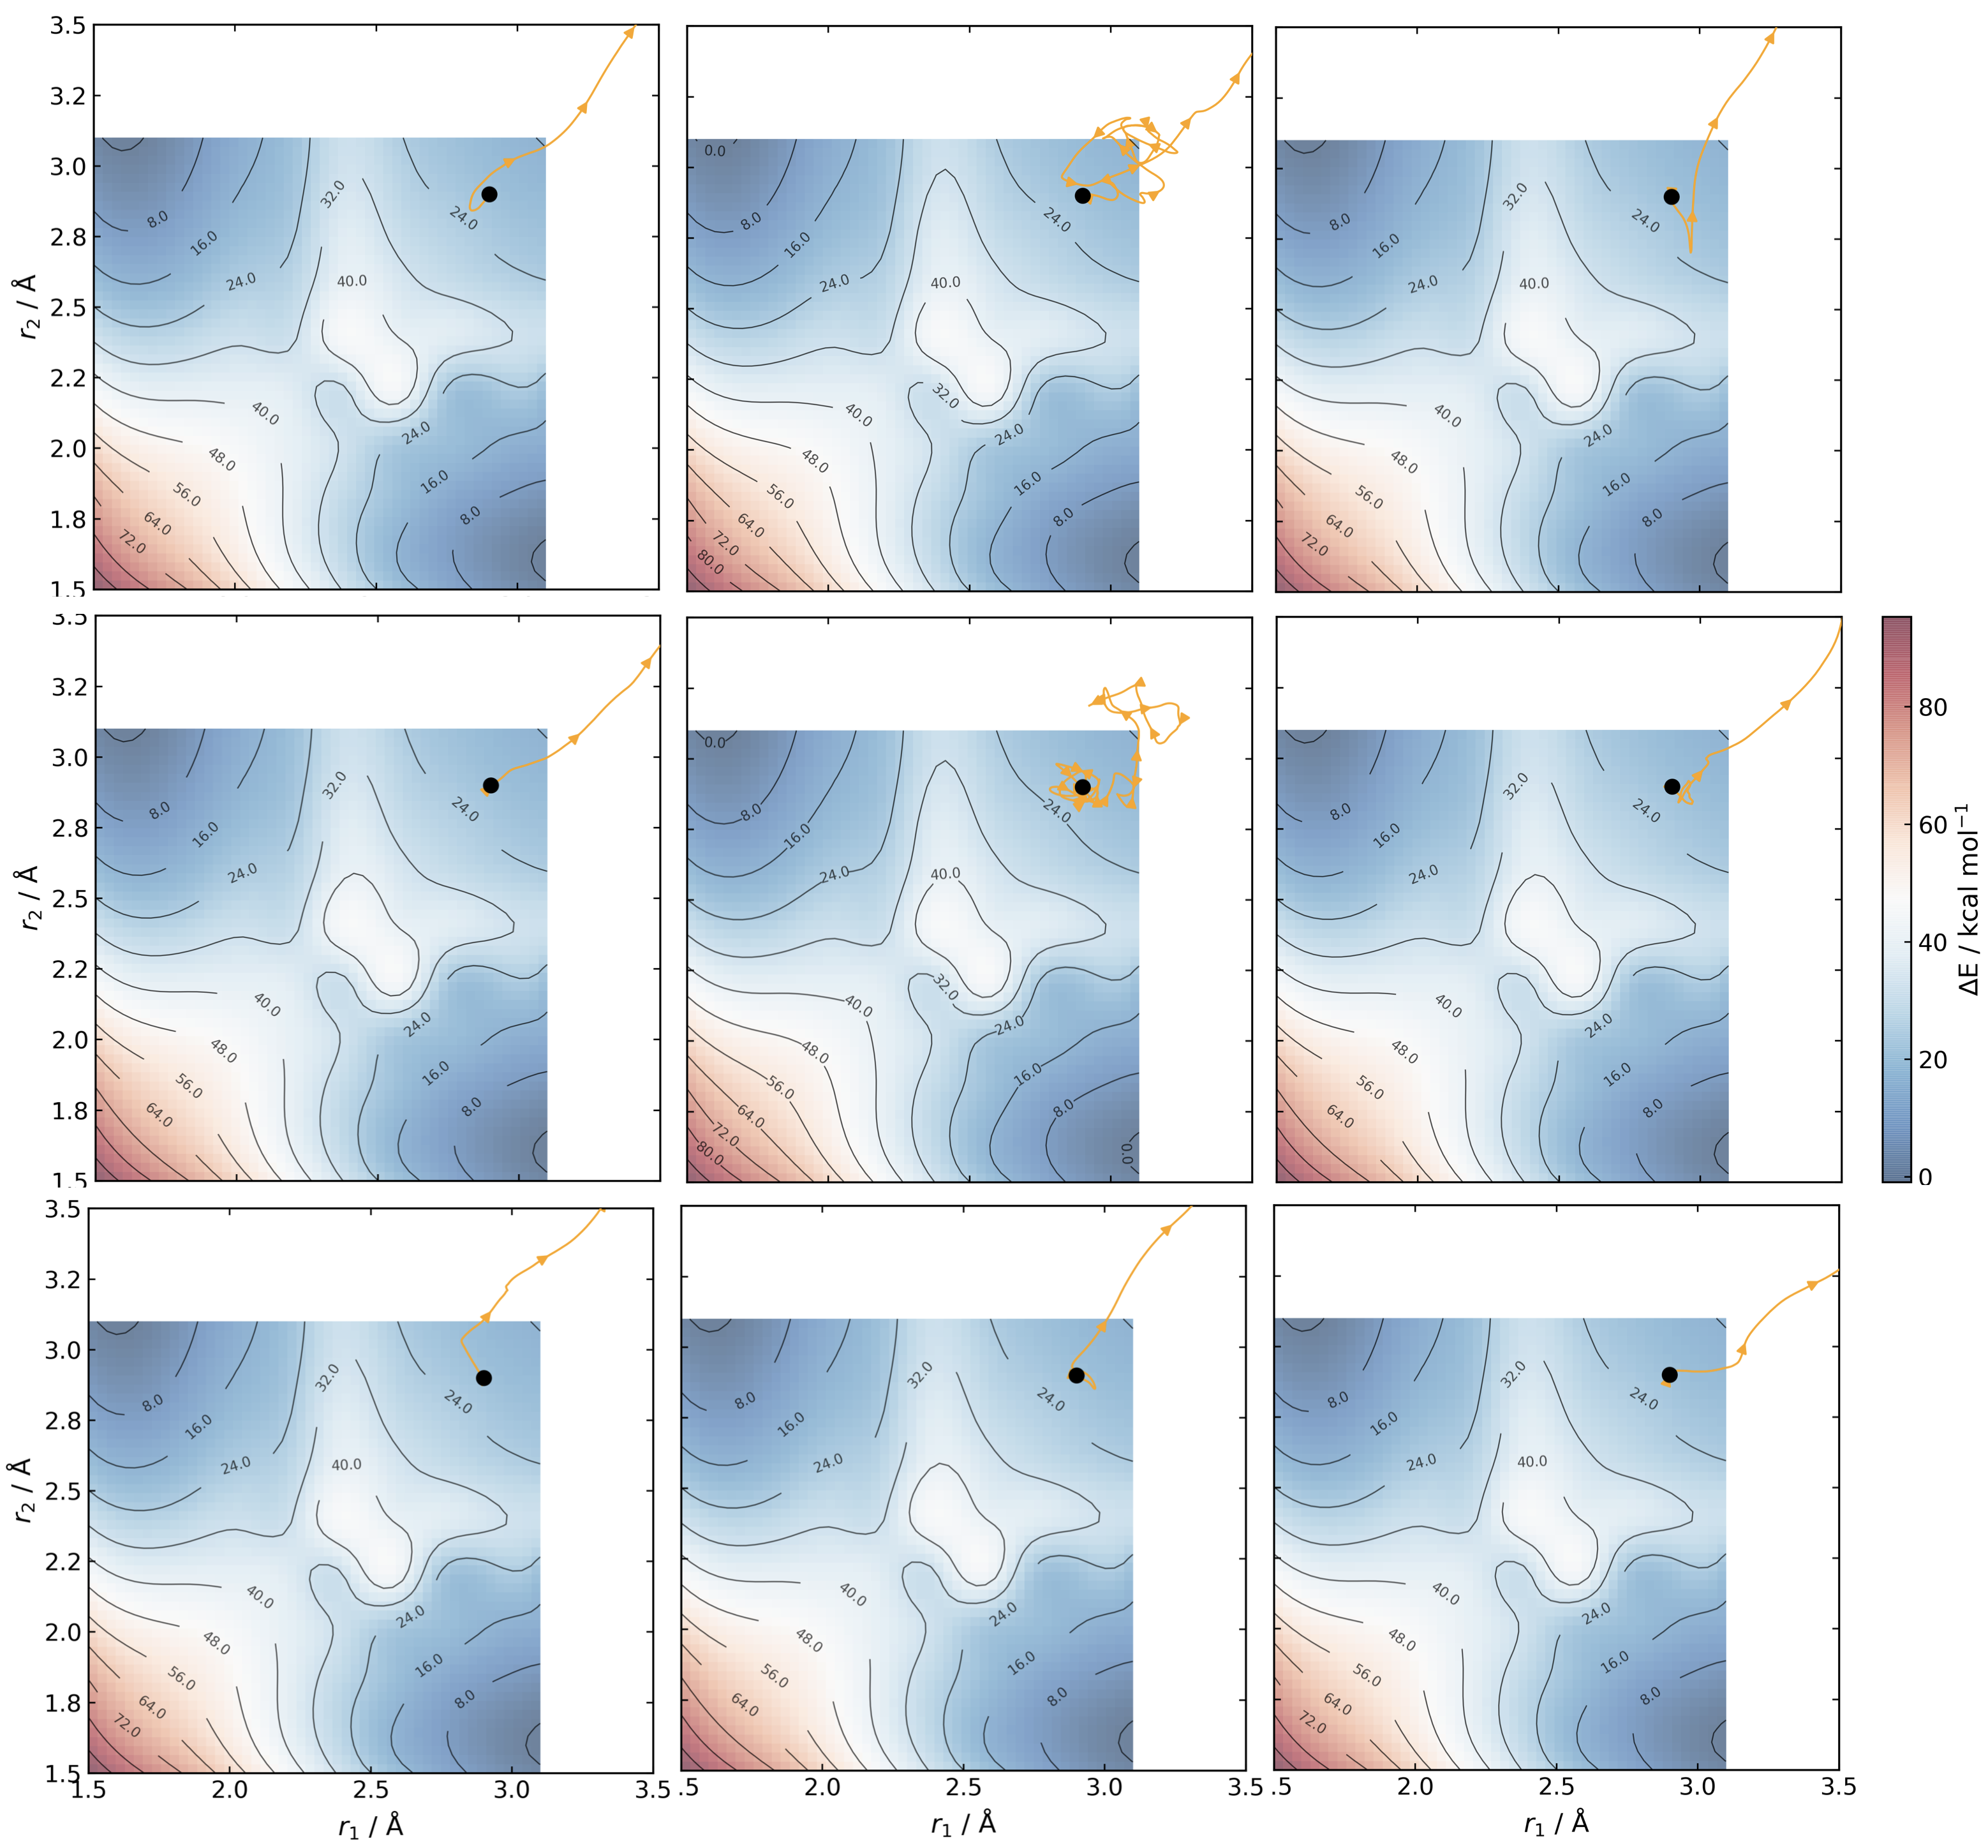
\includegraphics[width=\textwidth]{6/gap/figs_si/fig18}
	\vspace{0.2cm}
	\hrule
	\caption{2D PES along the forming bond distances ($r_1, r_2$) in the [4+2] dimerisation of cyclopentadiene as a function of time. GAP–propagated reactive dynamics (300 K, yellow lines) overlaid on the relaxed 2D PES. TS$_1$ (7N in ref. \cite{Caramella2002}) is shown as the black point. All trajectories lead to reactants (cyclopentadiene $\times$ 2) after $\sim$100 fs. GAP trained on ground truth B3LYP/def2-SVP. Active learning performed at 500 K initiated at $r_1, r_2$ = 2.9 \AA.}
	\label{fig::ml_si_18}
\end{figure}


\begin{figure}[h!]
	\vspace{0.4cm}
	\centering
	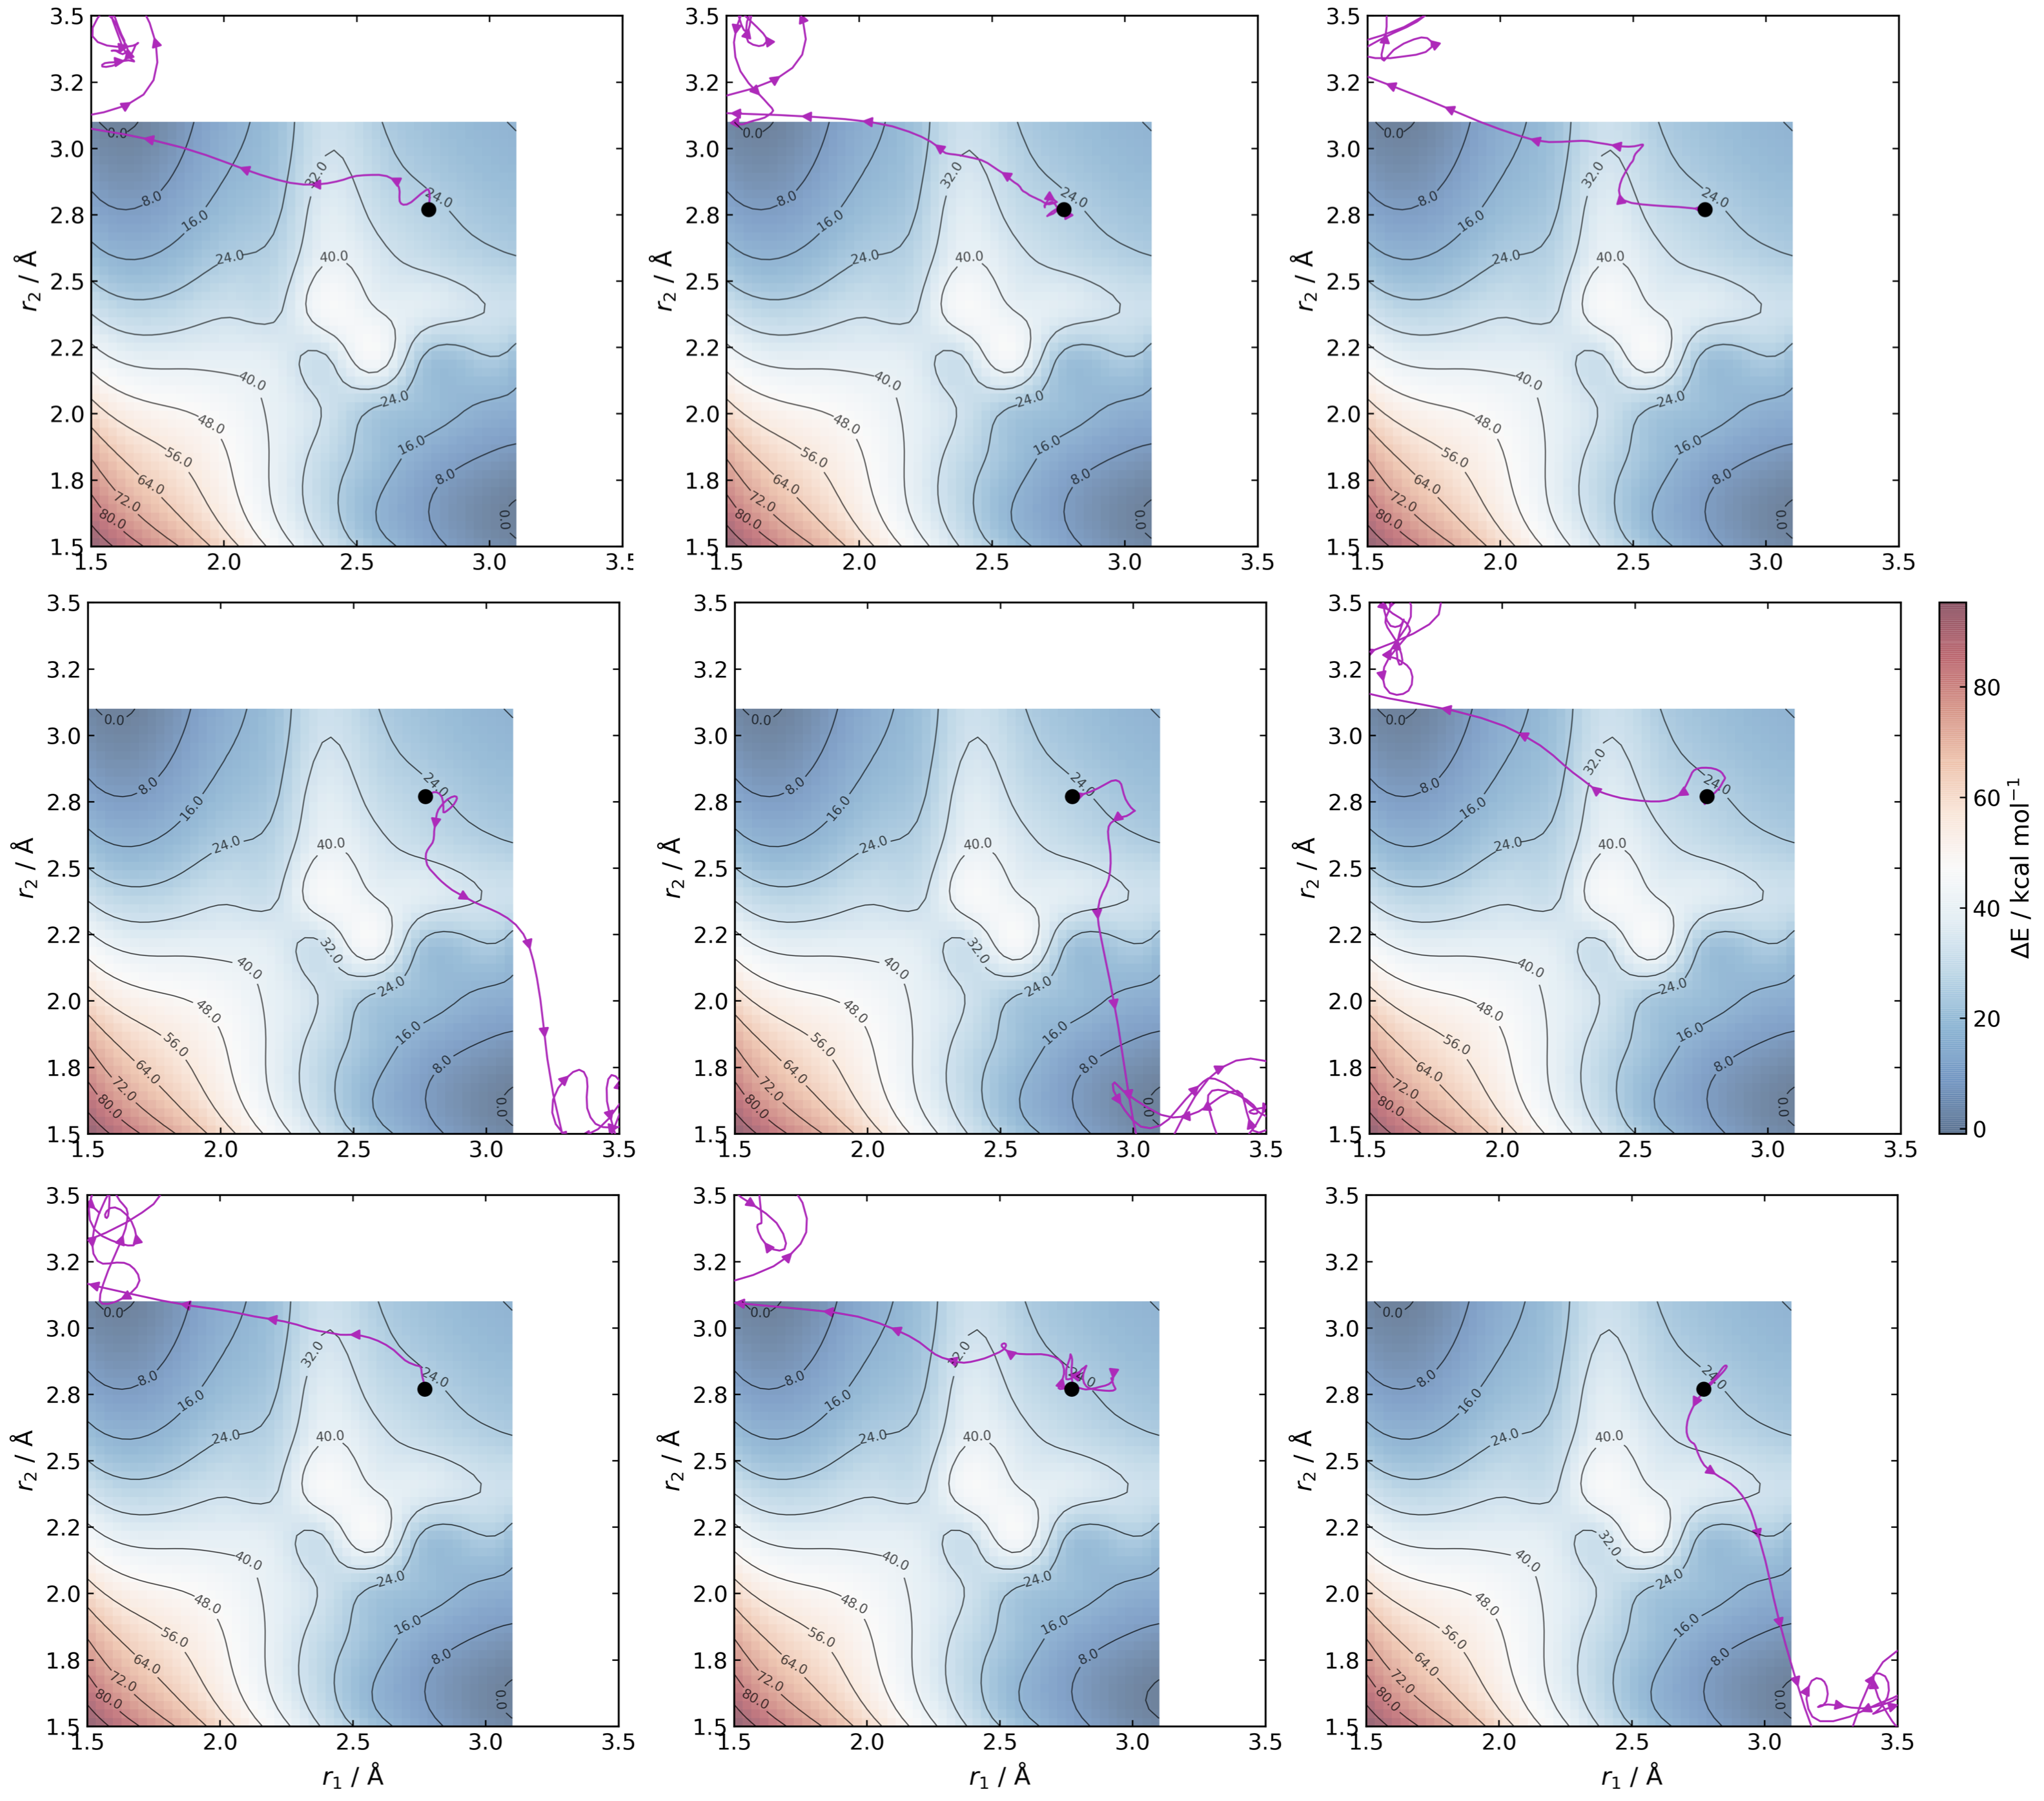
\includegraphics[width=\textwidth]{6/gap/figs_si/fig20}
	\vspace{0.2cm}
	\hrule
	\caption{As Figure \ref{fig::ml_si_18} but GAP active learning then dynamics initiated from TS${}_1’$ ($r_1,, r_2$ = 2.77 \AA.}
	\label{fig::ml_si_20}
\end{figure}



\begin{figure}[h!]
	\vspace{0.4cm}
	\centering
	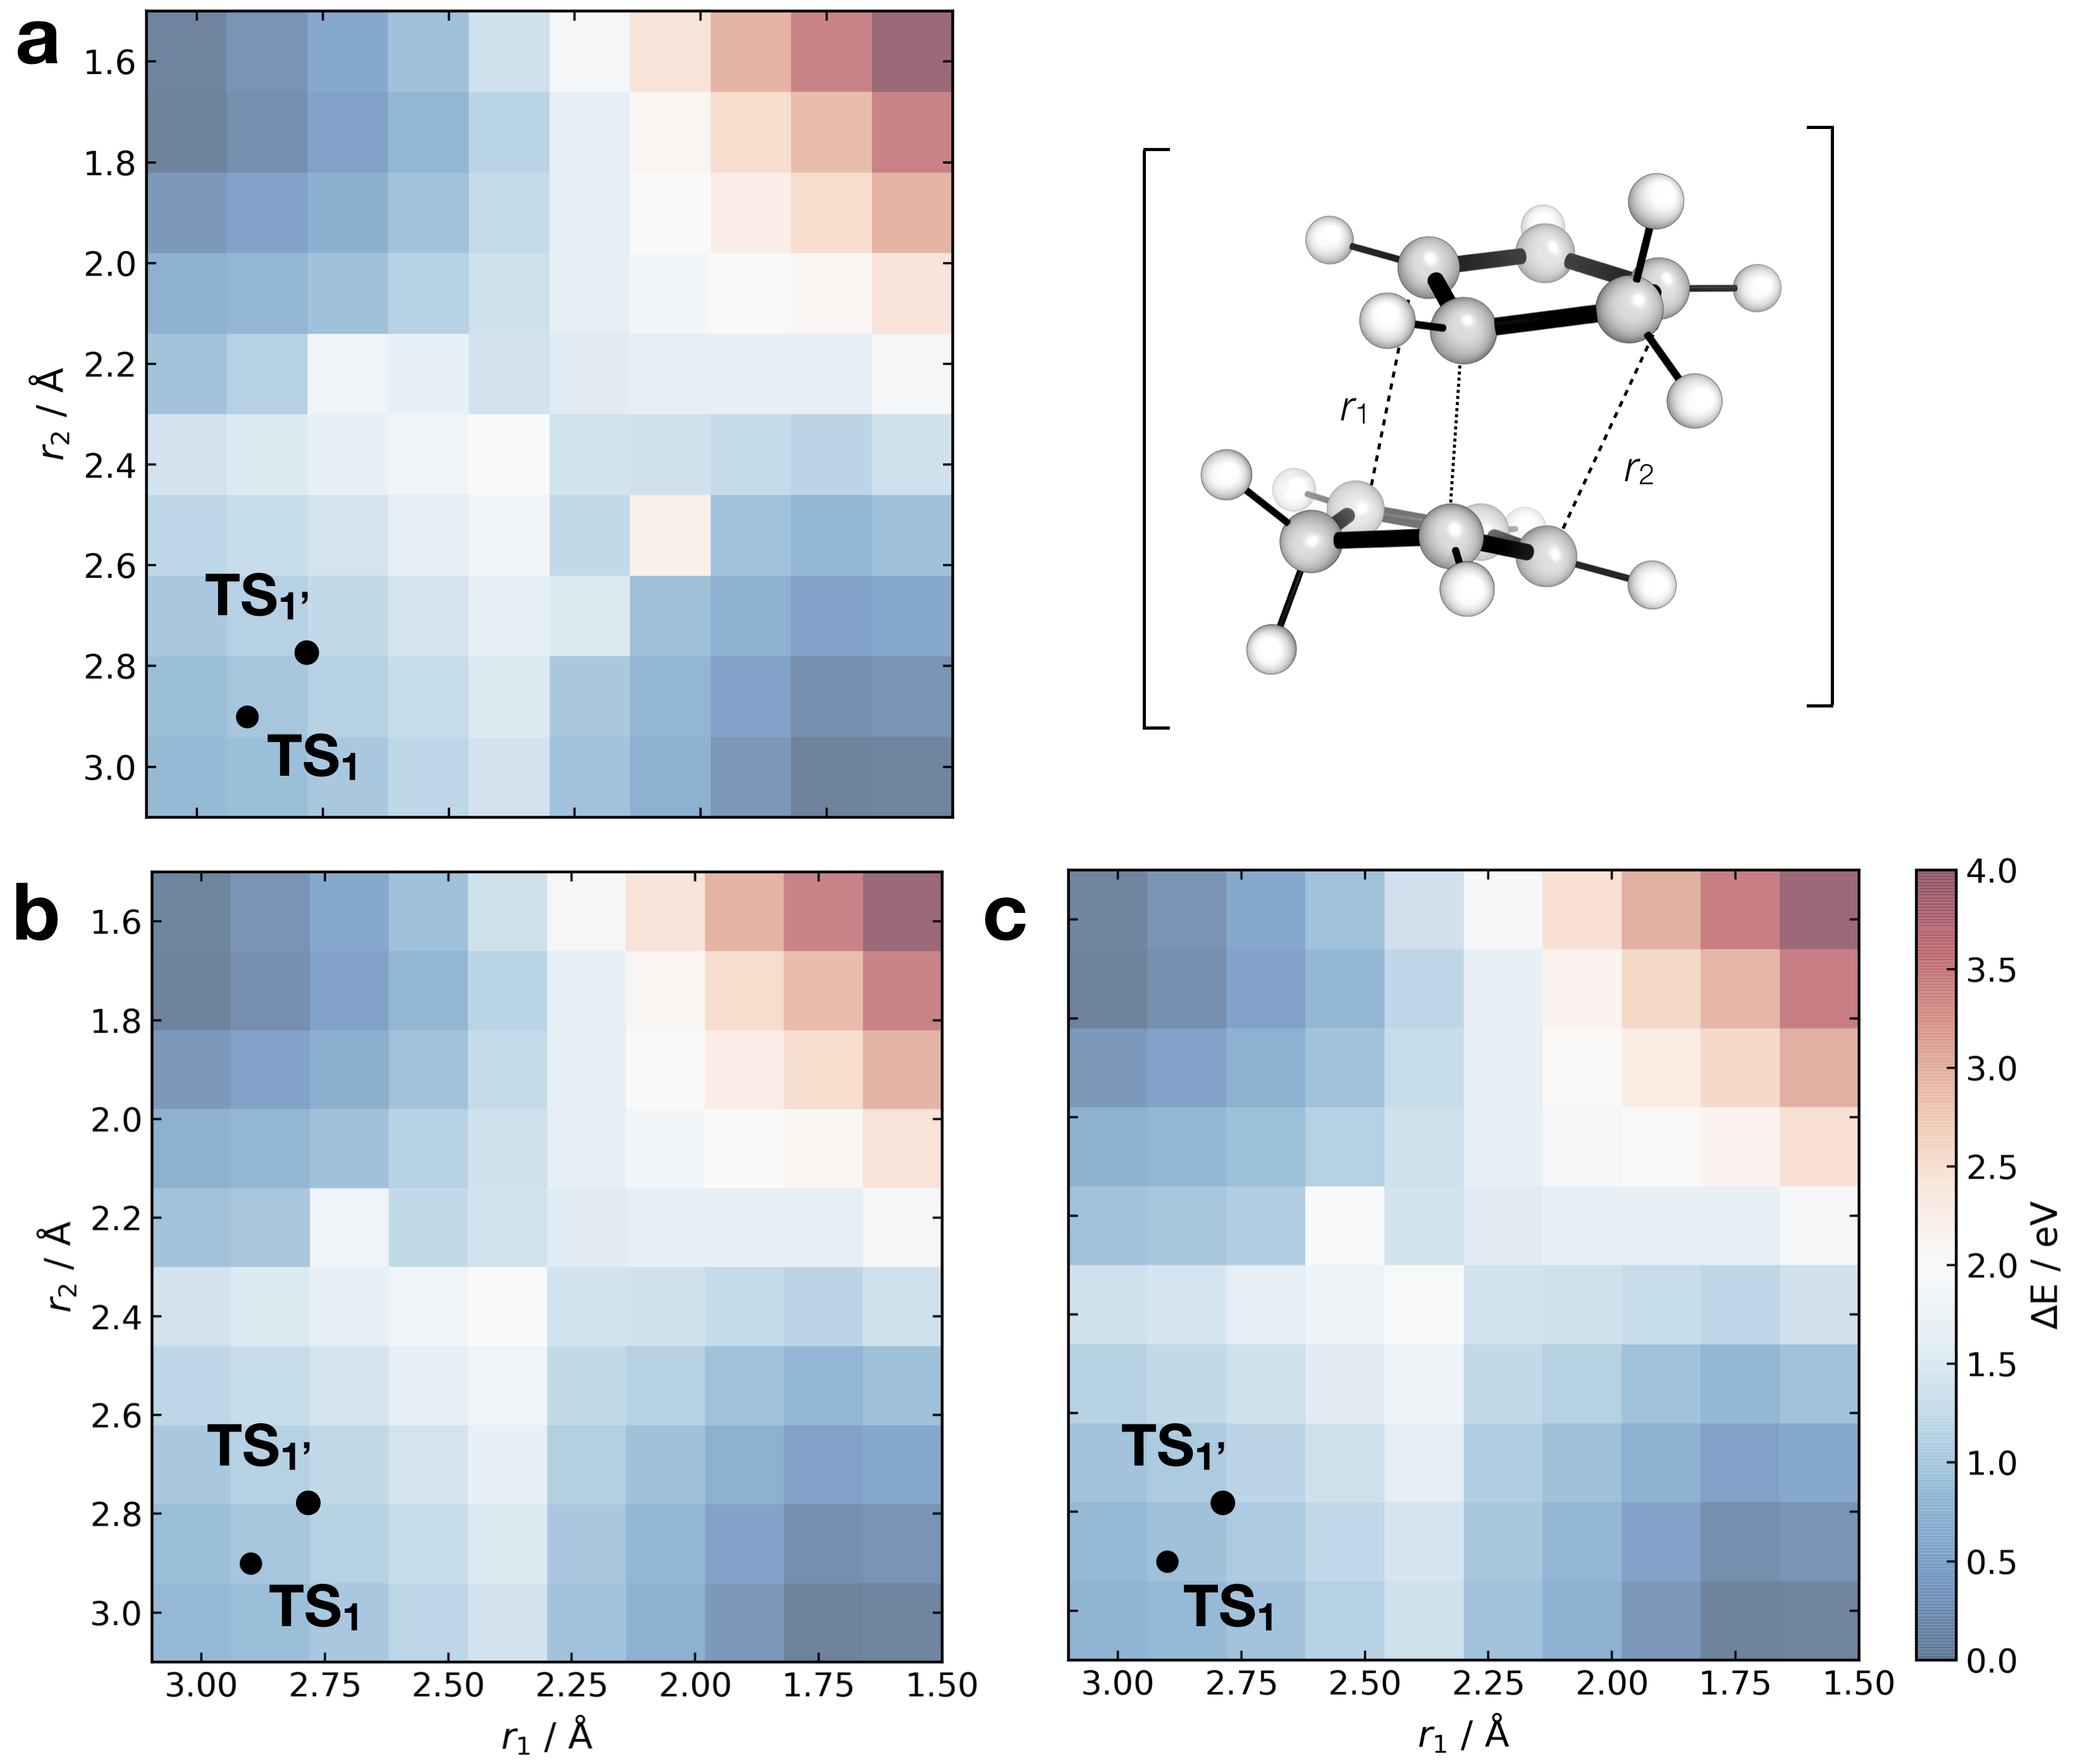
\includegraphics[width=0.9\textwidth]{6/gap/figs_si/fig21}
	\vspace{0.2cm}
	\hrule
	\caption{Comparison of 2D relaxed potential energy surfaces at (a) B3LYP/6-31G(d) as reported in ref. \cite{Caramella2002} and (b) a slightly improved level, B3LYP/def2-SVP.}
	\label{fig::ml_si_21}
\end{figure}


\begin{figure}[h!]
	\vspace{0.4cm}
	\centering
	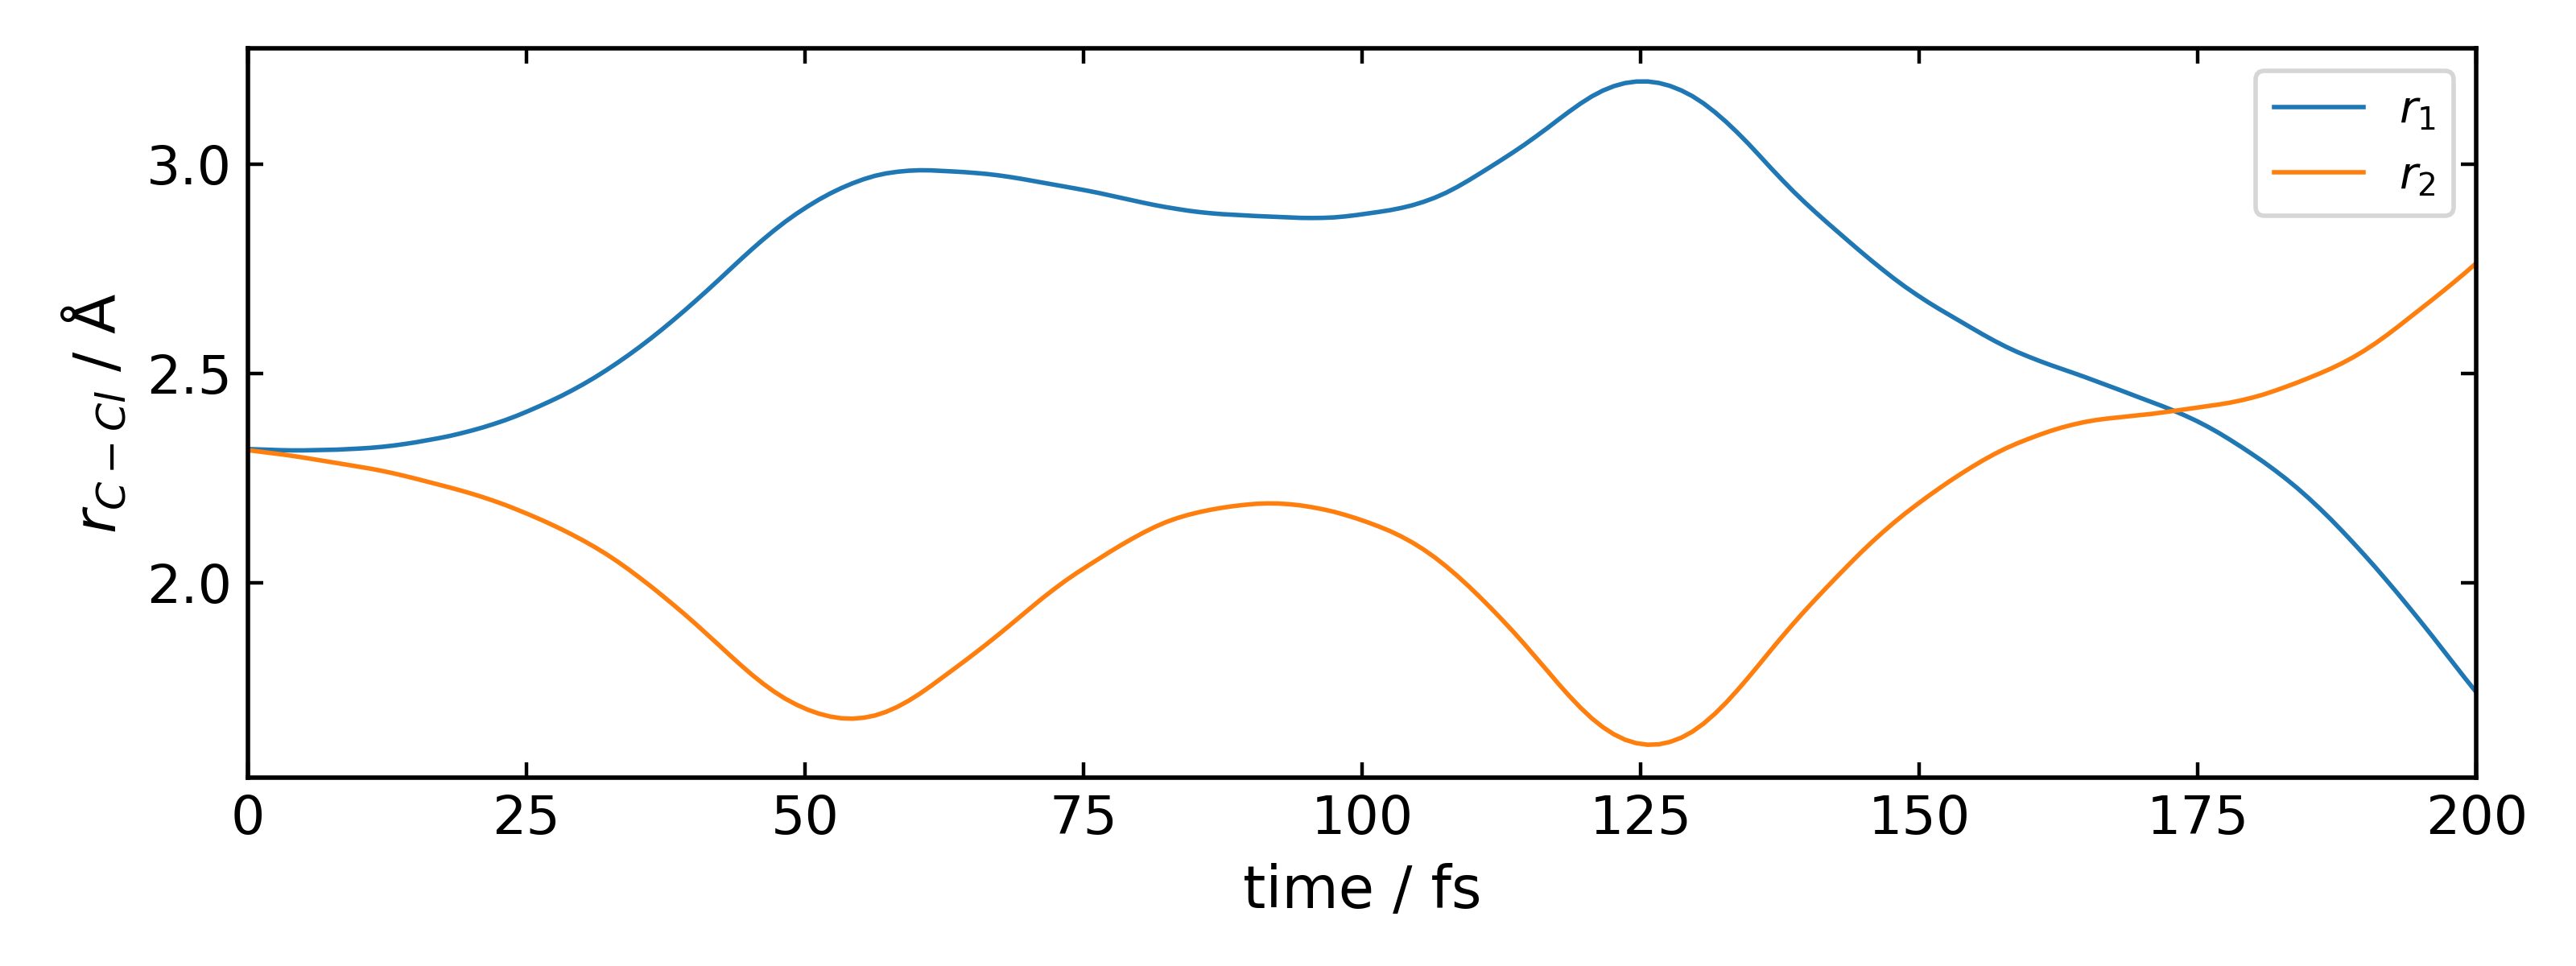
\includegraphics[width=11.5cm]{6/gap/figs_si/fig22}
	\vspace{0.2cm}
	\hrule
	\caption{C-Cl distances as a function of time for one of the ten GAP-MD propagated from the TS of Cl+CH${}_3$Cl in explicit water. A barrier recrossing event is observed at $\sim$170 fs.}
	\label{fig::ml_si_22}
\end{figure}



\begin{figure}[h!]
	\vspace{0.4cm}
	\centering
	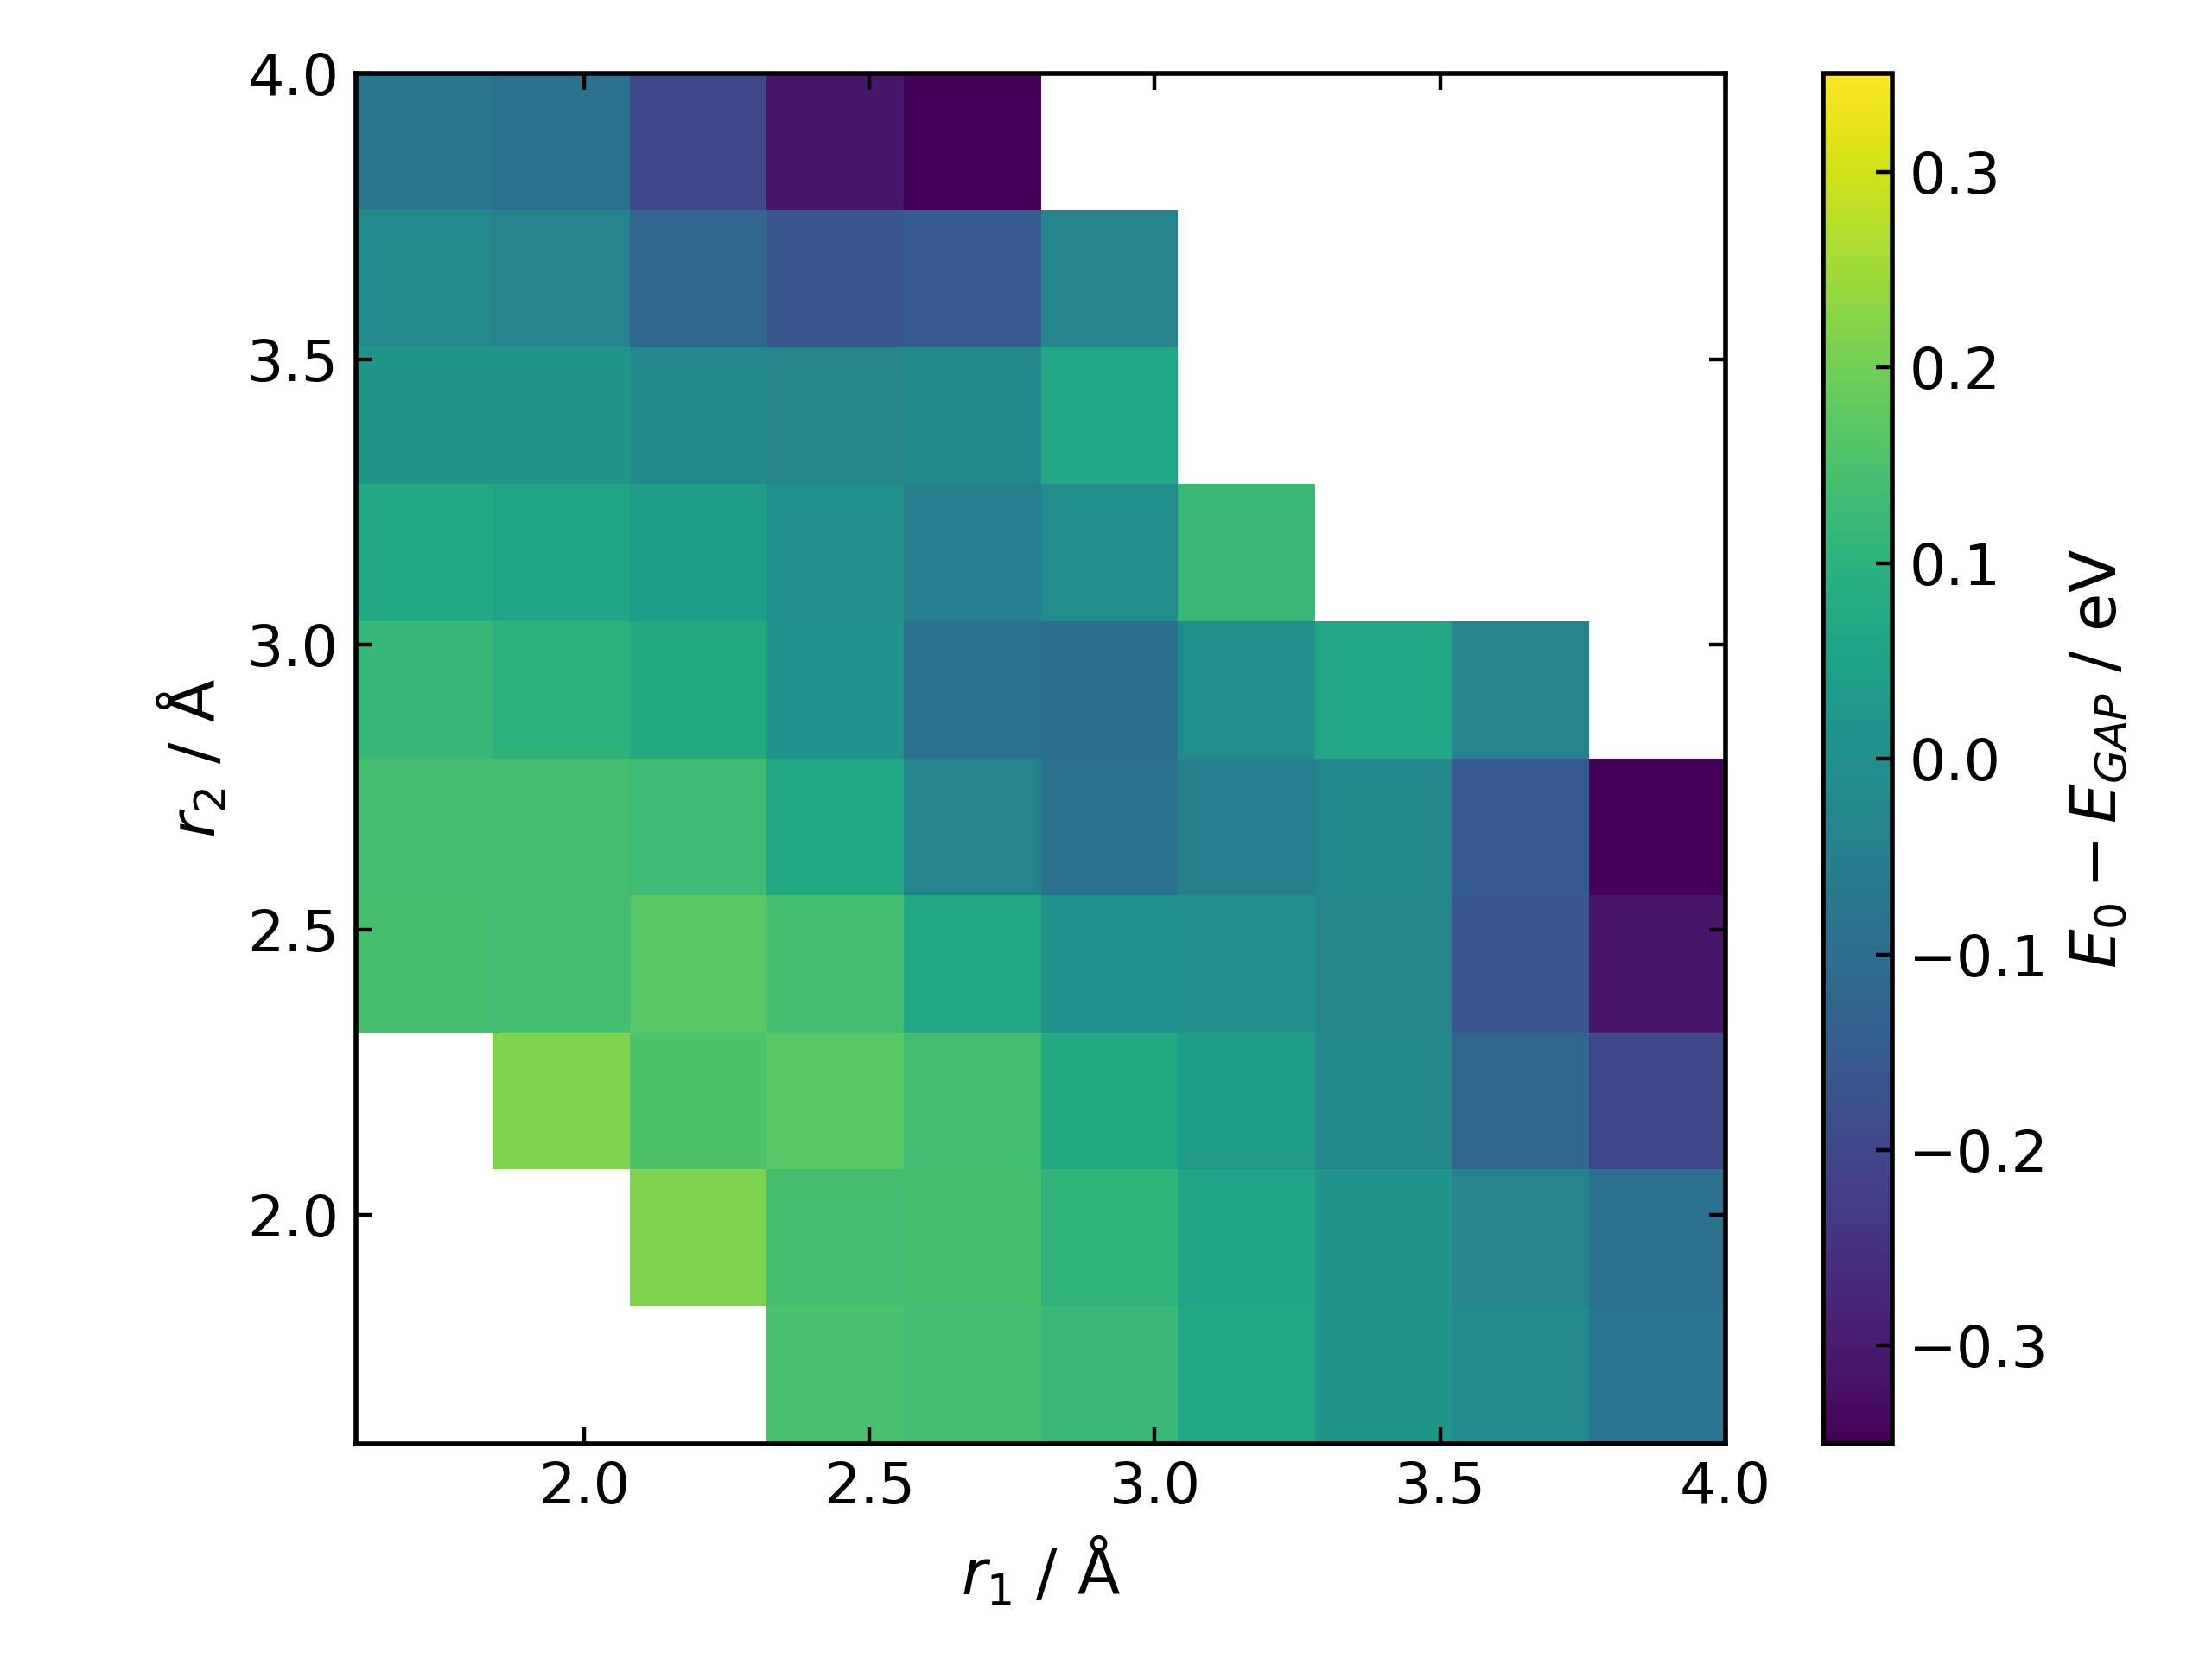
\includegraphics[width=10.5cm]{6/gap/figs_si/fig23}
	\vspace{0.2cm}
	\hrule
	\caption{Error between GAP predicted and ground truth (CPCM(Water)-PBE/def2-SVP) referenced to the closest point on the surface to the TS ($r_1, r_2 $ = 2.4 \AA) i.e. the starting point for the GAP active learning at 1600 K. Regions above 2 eV on the ground truth surface masked, as the training explicitly does not include any configurations $>$2eV from the minimum. }
	\label{fig::ml_si_23}
\end{figure}



\begin{figure}[h!]
	\vspace{0.4cm}
	\centering
	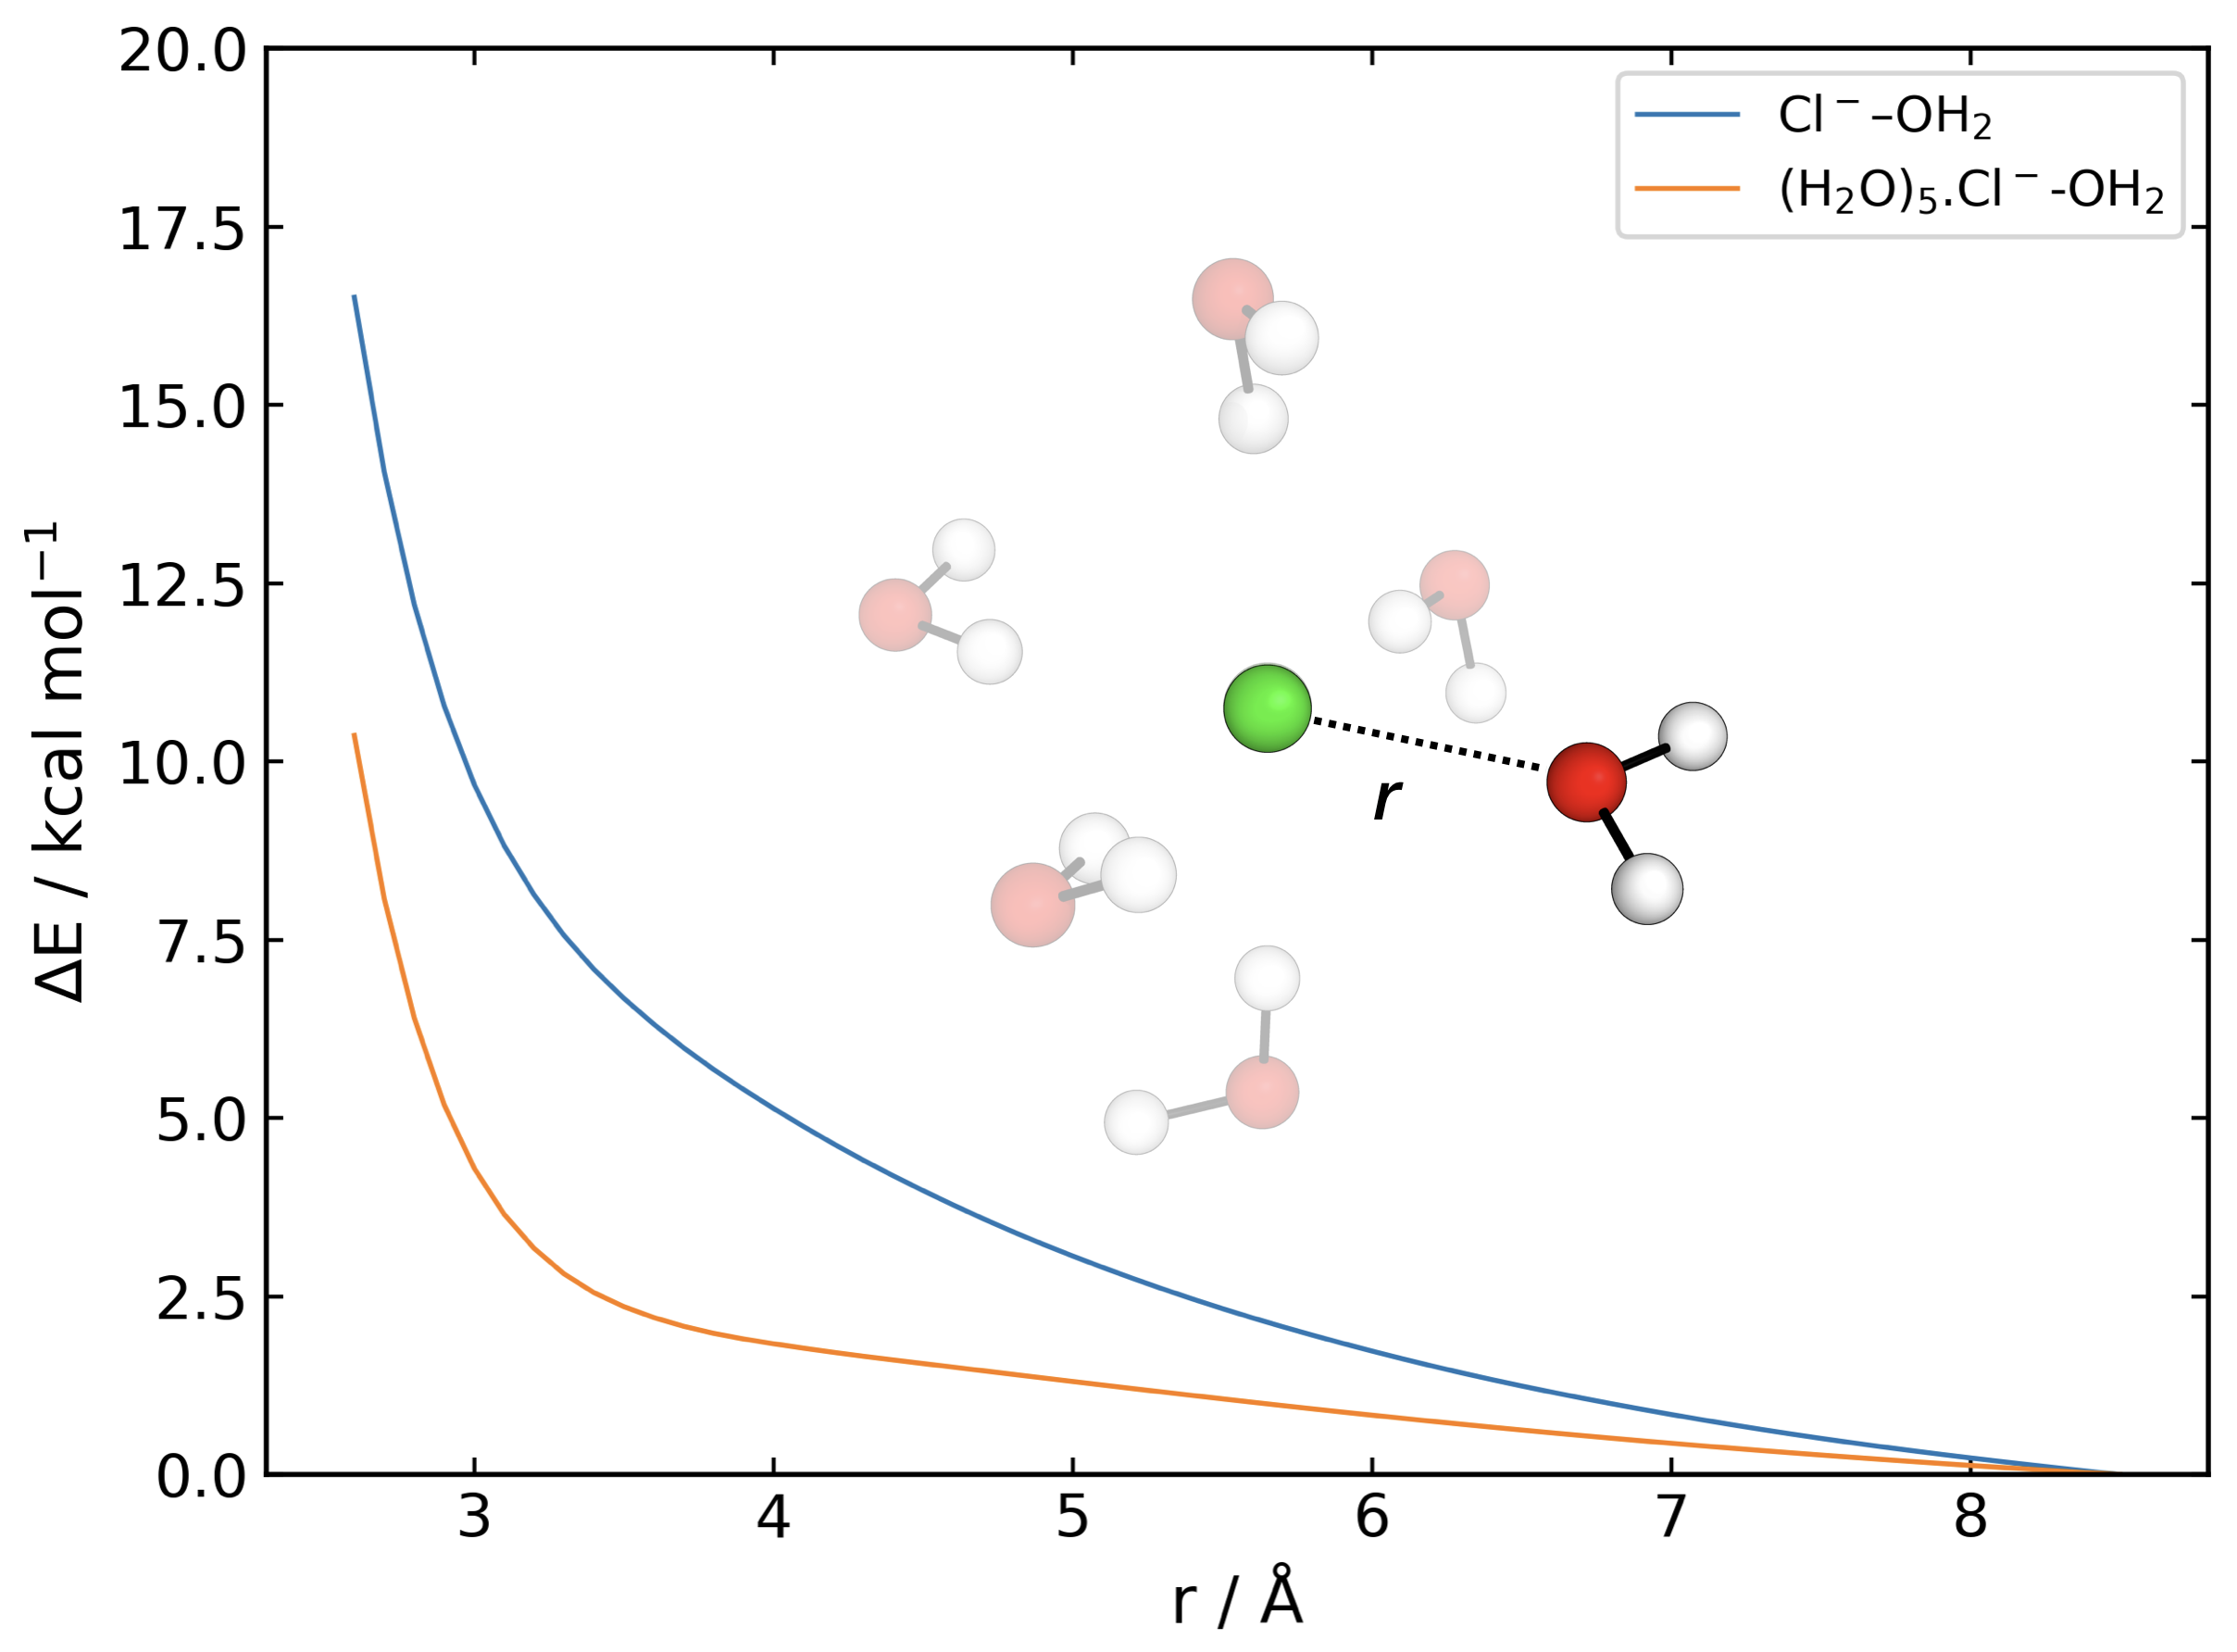
\includegraphics[width=10.5cm]{6/gap/figs_si/fig24}
	\vspace{0.2cm}
	\hrule
	\caption{Gas-phase potential energy surfaces for Cl${}^{-}\cdots$H$_{2}$O, with and without a first solvation shell at PBE/ma-def2-TZVP. Coordination number of chloride is 6 from ref. \cite{Busch2013}. Initial partially solvated chloride generated by hand and optimised with ORCA constraining the Cl--O distance and the O--Cl--O angles to generate a close to octahedral geometry. The solvated ion shows a faster decaying potential; based on this model and $r_c^\text{SOAP}$ = 4.5 \AA was chosen as a compromise between efficiency and accuracy.}
	\label{fig::ml_si_24}
\end{figure}




\begin{figure}[h!]
	\vspace{0.4cm}
	\centering
	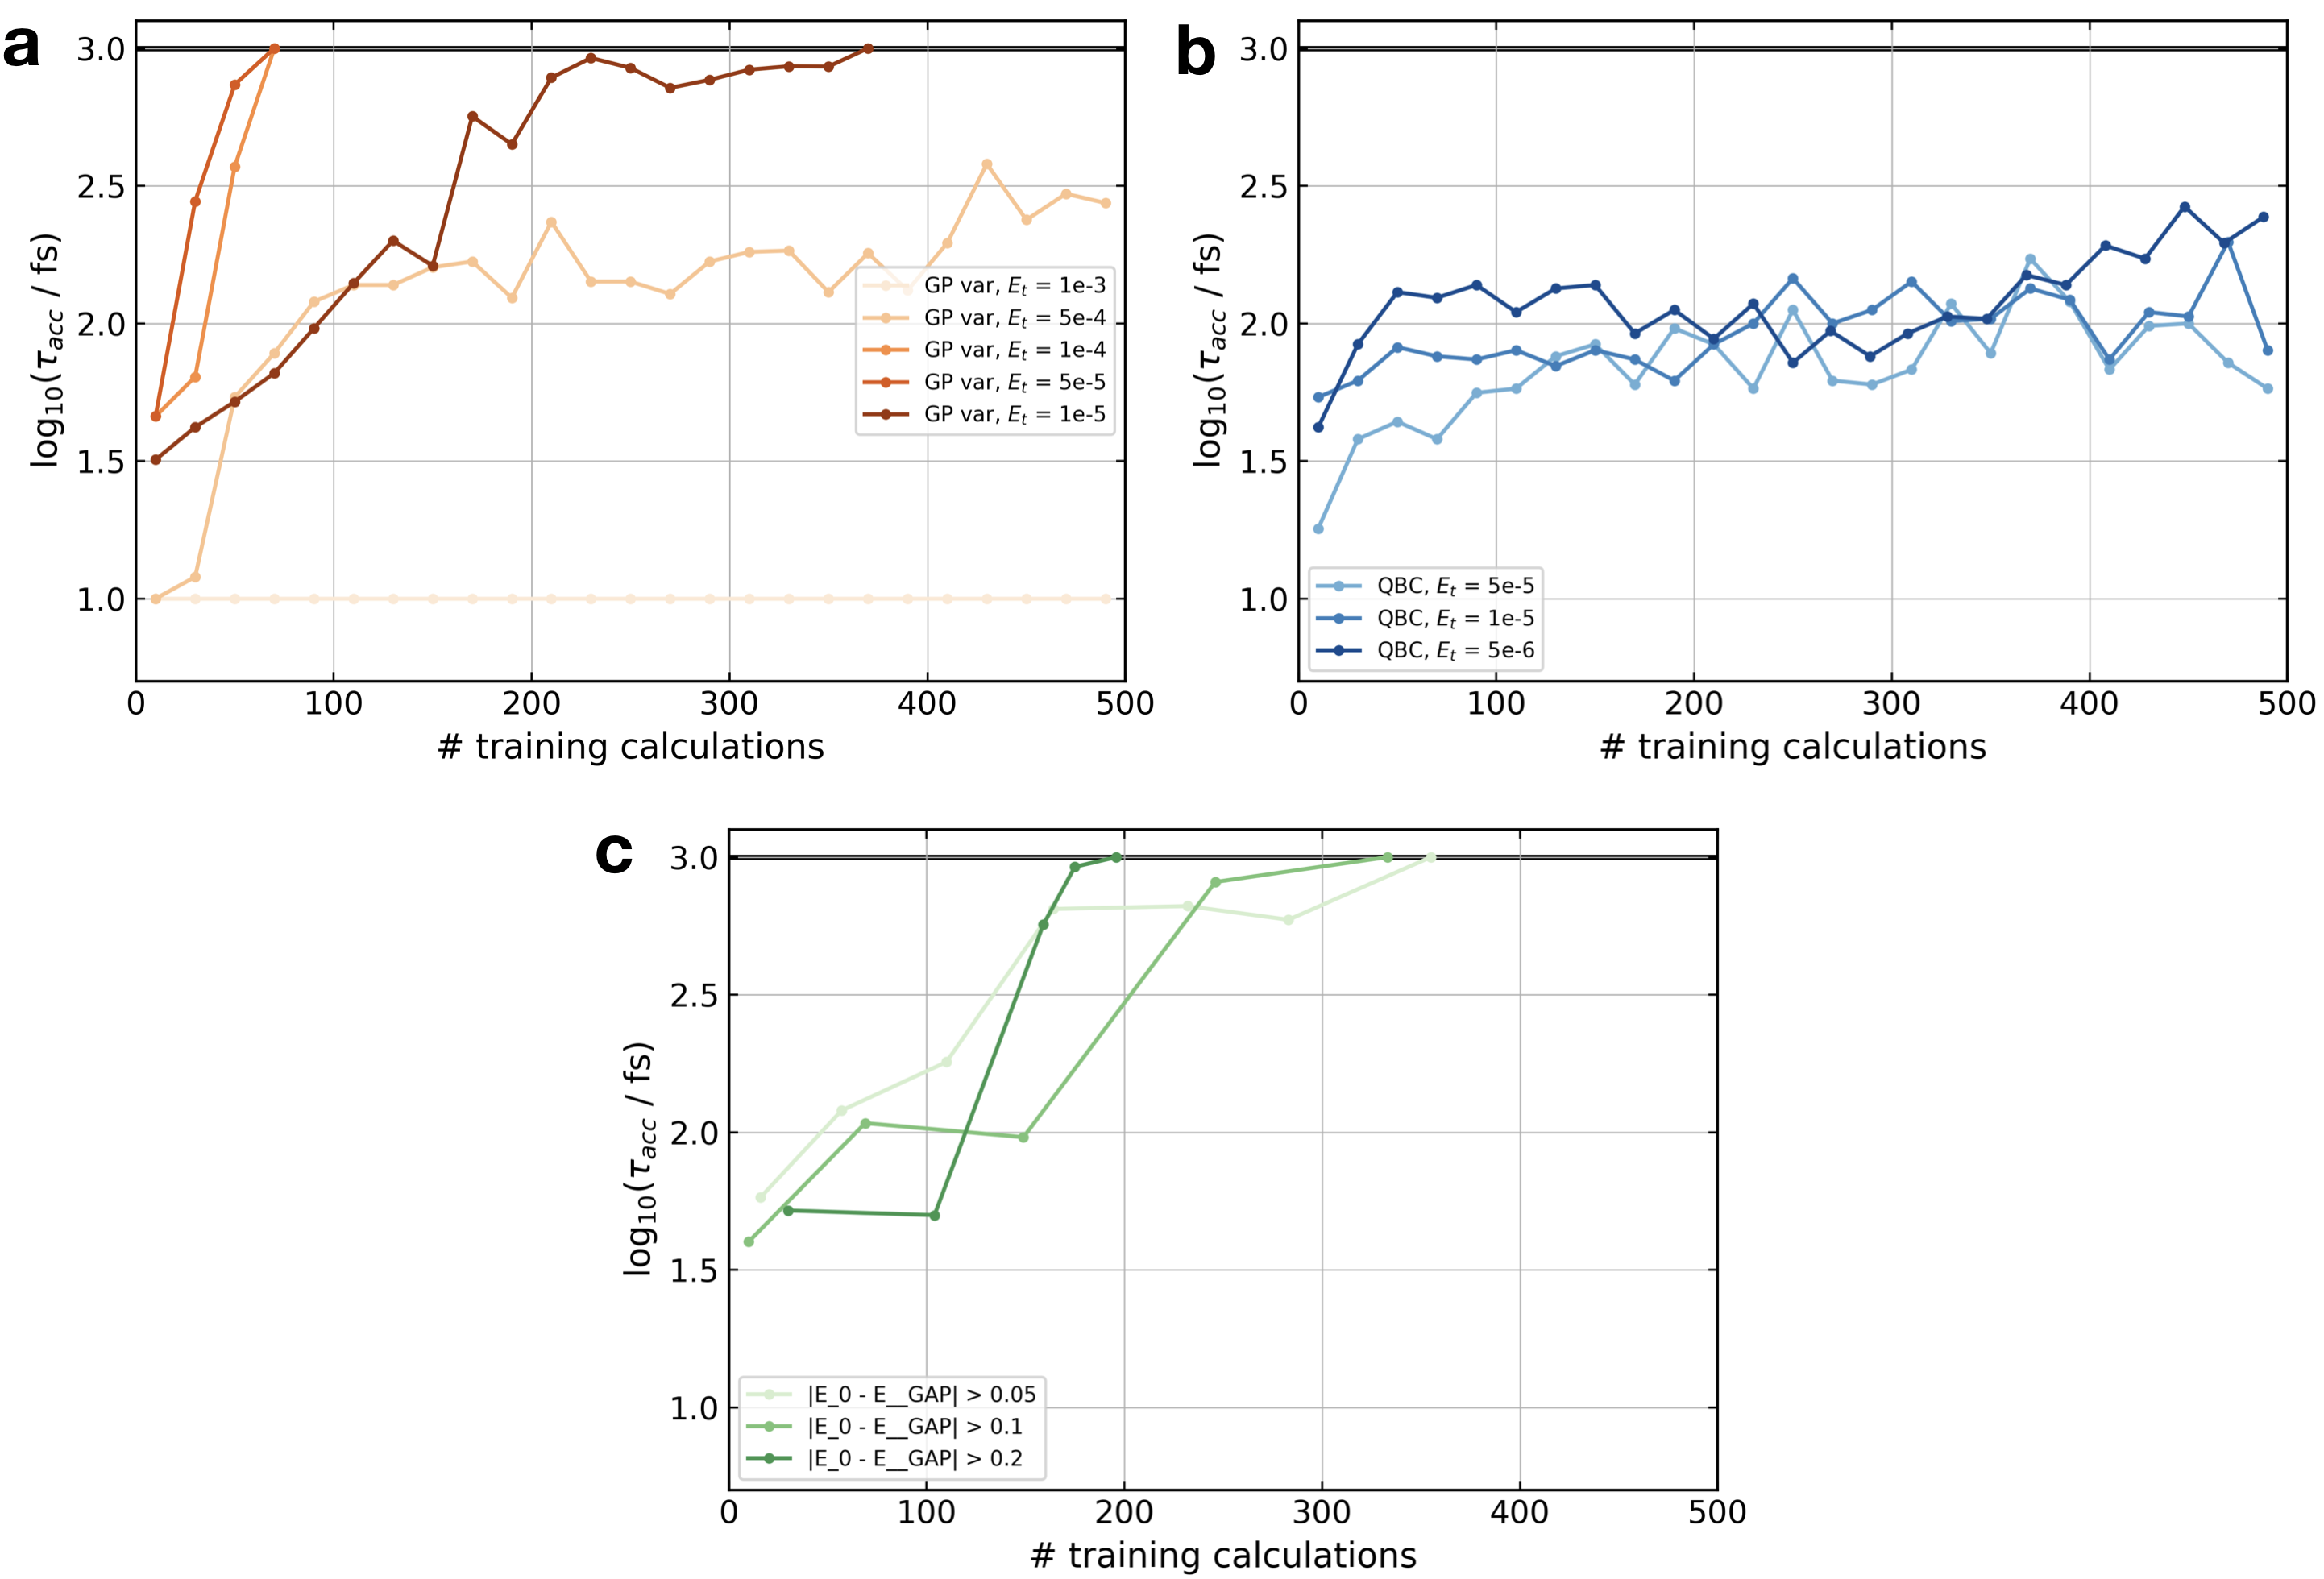
\includegraphics[width=\textwidth]{6/gap/figs_si/fig25}
	\vspace{0.2cm}
	\hrule
	\caption{Comparison of selection strategies used in the ‘active’ learning loop for the intermolecular component of a water GAP trained in a 7 \AA cubic box with 10 waters at the DFTB(3ob) level of theory. GAP-MD performed at 300 K with a 0.5 fs timestep for $n^3+2$ fs iterations sequentially until 1 ps of dynamics was performed. \taua used a 0.1 eV lower energy threshold and 1 eV total averaged over 5 random initial configurations (identical for each learning curve). (a) Adds a configuration when the maximum atomic energy variance predicted by the Gaussian Process exceeds a threshold $E_t$ (in eV, where the max is taken over all the atoms in a frame of GAP-MD). (b) Query-by-committee (QBC), where a configuration is added if the standard deviation between GAPs trained on the same data (with different random noise) exceeds a threshold Et (in eV). Values are chosen to span where the first frame from the iterative GAP-MD is chosen to the maximum 1ps allowed. (c) Adds a configuration where the true difference of the total energy exceeds a threshold (in eV).}
	\label{fig::ml_si_25}
\end{figure}








\clearpage
\end{document}